\documentclass[12pt, a4paper, twoside]{book}

\title{Computable characterisations of stochastic uncertainty in differential equations}
\author{Liam Blake}
\date{\today}
\def\degree{Master of Philosophy}
\def\discipline{Applied Mathematics}


\usepackage{thesis}

% \RequirePackage[authoryear,sort,comma]{natbib}
% \setcitestyle{authoryear,aysep={}}
% TODO: Need to ensure that all names are written out fully, so don't have to set uniquename.
% e.g. if the bibliography includes A. Stuart and Andrew Stuart, the two names will be written out in FULL when citing.
\RequirePackage[
	backend=biber,
	natbib,
	style=authoryear-comp,
	maxcitenames=2,
	mincitenames=1,
	maxbibnames=4,
	minbibnames=3,
	giveninits=true,
	uniquename=init,
	sorting=ynt,
	date=year
]{biblatex}

% Ensure initials are always listed first
\DeclareNameAlias{sortname}{first-last}

% Fix to link the name as well in citations - https://tex.stackexchange.com/questions/15951/hyperlink-name-with-biblatex-authoryear-biblatex-1-4b/27107#27107
% \DeclareFieldFormat{citehyperref}{%
%   \DeclareFieldAlias{bibhyperref}{noformat}% Avoid nested links
%   \bibhyperref{#1}}

% \DeclareFieldFormat{textcitehyperref}{%
%   \DeclareFieldAlias{bibhyperref}{noformat}% Avoid nested links
%   \bibhyperref{%
%     #1%
%     \ifbool{cbx:parens}
%       {\bibcloseparen\global\boolfalse{cbx:parens}}
%       {}}}

% \savebibmacro{cite}
% \savebibmacro{textcite}

% \renewbibmacro*{cite}{%
%   \printtext[citehyperref]{%
%     \restorebibmacro{cite}%
%     \usebibmacro{cite}}}

% \renewbibmacro*{textcite}{%
%   \ifboolexpr{
%     ( not test {\iffieldundef{prenote}} and
%       test {\ifnumequal{\value{citecount}}{1}} )
%     or
%     ( not test {\iffieldundef{postnote}} and
%       test {\ifnumequal{\value{citecount}}{\value{citetotal}}} )
%   }
%     {\DeclareFieldAlias{textcitehyperref}{noformat}}
%     {}%
%   \printtext[textcitehyperref]{%
%     \restorebibmacro{textcite}%
%     \usebibmacro{textcite}}}

\bibliography{thesis}


% \includeonly{chp07_outlook/outlook,appendix/epidemiology}

\begin{document}
% \emergencystretch 3em

%!TEX root = thesis.tex

\frontmatter
\maketitle

{
	\hypersetup{linkcolor=black}
	\microtypesetup{deactivate}

	\tableofcontents

	\listoffigures
	\microtypesetup{reactivate}
}


% Frontmatter
%!TEX root = ../thesis.tex
\chapter{Abstract}
\small
Differential equations are used ubiquitously to predict and understand phenomena across many fields.
These models are inevitably subject to uncertainties arising from a range of sources, including measurement error, unresolved components, and resolution limitations.
Accounting for these uncertainties leads to better models, but this is analytically challenging and often requires computationally expensive Monte Carlo simulation.
In this thesis, we consider It\^o stochastic differential equations, which extend ordinary differential equations to include stochastic terms and provide a rich framework for explicitly parameterising uncertainties in the model.
We look to address the need for computationally efficient methods that characterise uncertainty without resorting to the alternative of bulk simulation.

We first build upon previous small-noise studies to provide an explicit bound for the error between stochastic differential equations and corresponding linearisations written in terms of a deterministic system.
Our framework accounts for non-autonomous coefficients, multiplicative noise, and uncertain initial conditions.
These linearisations are solvable and efficient to compute and so can serve as an approximate solution to the stochastic differential equation.
We demonstrate the predictive power of our bound on several toy examples, providing for the first time a numerical validation of linearisation approximations of stochastic differential equations.
In characterising this relationship, we are also able to extend stochastic sensitivity (Balasuriya, \emph{SIAM Review}, 2020:781-816), a recently introduced tool for characterising the impact of uncertainty on differential equation solutions.
Stochastic sensitivity was previously restricted to 2-dimensional flows and we overcome this limitation to empower the use of these tools on models of arbitrary dimension.

We also propose an \emph{ad hoc} algorithm for approximating a stochastic differential equation solution with a Gaussian mixture model constructed from many different linearisations.
Such an algorithm is computationally efficient and provides an analytic probability density function, unlike stochastic samples.
Critically, the algorithm can capture non-Gaussian features in the stochastic solution that a single linearisation cannot.
Our initial investigation into this algorithm, using a data-driven model of a drifter in the Gulf Stream, yielded promising results to motivate future development.

Our work provides many avenues for further development, some of which we discuss briefly.
This includes theoretical extension to a broader range of stochastic models driven by different types of noise and implications for the Fokker-Planck equation, an equivalent representation of a stochastic differential equation.
We also anticipate applications within the fields of data assimilation, stochastic parameterisation, and, through a connection with results for discrete stochastic systems, mathematical epidemiology.

%!TEX root = ../thesis.tex
\chapter{Signed Statement}
 {
  I certify that this work contains no material which has been accepted for the award of any other degree or diploma in my name, in any
  university or other tertiary institution and, to the best of my knowledge and belief, contains no material previously published or written by
  another person, except where due reference has been made in the text. In addition, I certify that no part of this work will, in the future, be used
  in a submission in my name, for any other degree or diploma in any university or other tertiary institution without the prior approval of the
  University of Adelaide and where applicable, any partner institution responsible for the joint award of this degree.

  I give permission for the digital version of my thesis to be made available on the web, via the University’s digital research repository, the
  Library Search and also through web search engines, unless permission has been granted by the University to restrict access for a period of
  time.

  I acknowledge the support I have received for my research through the provision of an Australian Government Research Training Program
  Scholarship

  \vspace{4ex}
  Signed: \dotfill\quad
  Date: \dotfill

 }

%!TEX root = ../thesis.tex
\chapter{Acknowledgements}
\label{ch:acknowledgements}

First and foremost, I give the uttermost gratitude to my two supervisors, Sanjeeva Balasuriya and Jack Maclean.
Our meetings were always interesting and enjoyable and throughout they had the utmost patience and reassurance for my many worries.
Sanjeeva was a
Jack provided but also a realism that helped keep us all in check.
They both made this work fun and I learnt so much about research from their unique approaches.

All of the maths HDRs made working on this project a blast, but I reserve particular gratitude for the Level 7 gang: Clover Hoffman, George Savvoudis, Irulan Murphy, Kai Li, Matthew Drown, Saka Magsarjav, Steven Greenwood, and Wills Nguyen.

I also want to thank all the legends within the ATCA teams at the Adelaide University Cricket Club, who will almost surely never read this disquisition but provided an incredibly valuable escape from it at trainings and during our matches.

To my closest friends (to follow a clich\'e, you all should know who you are), thank you for all the coffees, the boardgames, the runs, and the drinks.
All these moments went a long way to keeping me sane.

Finally, to my parents Alison and Stephen, and my grandmother Margaret, thank you always for your ongoing love and support.

% \include{front/dedication}

\mainmatter

% Chapters
%!TEX root = ../thesis.tex

\chapter{Introduction}\label{ch:intro}
Many phenomena across geophysical, biological and socio-economic applications can be modelled using ordinary differential equations (ODEs).
Given an initial condition, these models can be solved, either analytically or numerically, to predict the behaviour at a future time.
These models are usually specified in a purely \emph{deterministic} fashion, in that each component is treated as being known exactly.
The model consequently provides a single prediction of the future state for any given initial condition.
However, in any modelling scenario, there will inevitably be uncertainty in the model specification which can arise from:
\begin{itemize}
	\item the model being sourced from measured data, which itself includes observational error
	\item information only being available on a spatiotemporal grid (resolution error), either due to data availability or discretisation of the model
	\item a lack of a complete understanding of all the processes involved in the system
	\item unknown values for any parameters in the model
	\item imperfect knowledge of the initial conditions.
\end{itemize}
Without appropriately accounting for these many manifestations of uncertainty, any predictions and inferences from the deterministic model may be inaccurate or even misleading.
This is not a trivial problem to resolve, however, as this uncertainty is inherently unknowable.
Even when the uncertainty cannot be directly encoded into the model, an understanding of how reliable the predictions of the model are in the presence of this uncertainty is extremely valuable.

This problem of uncertainty plague every field, but has received particular attention in climate modelling and weather prediction.
For example, resolution issues pose a significant challenge in producing accurate predictions from a high-dimensional climate model.
Many such models rely upon a spatial discretisation for tractable analysis and simulation, which in turn often requires an extremely high resolution to produce accurate simulations that correctly capture all relevant processes \citep{DawsonEtAl_2012_SimulatingRegimeStructures}.
Without even considering the plethora of other sources of uncertainty in climate modelling, the discretisation of the model that is necessary for tractability introduces resolution issues that require a high computational load to overcome.

One approach to systematically account for uncertainty is by replacing the deterministic model with a \emph{stochastic} one, where the uncertainty is introduced as an inherent part of the model and the solutions are treated as random quantities.
The formal introduction of stochastic terms to account for unknown and unresolved processes into an otherwise deterministic model is known as \emph{stochastic parameterisation} in scientific circles \citep{BernerEtAl_2017_StochasticParameterizationNew,Palmer_2019_StochasticWeatherClimate}.
Stochastic parameterisation has been shown to both lead to the same performance as higher-resolution models---\citet{DawsonPalmer_2015_SimulatingWeatherRegimes} showed through simulation studies that the performance of a high-resolution purely deterministic model can be matched by a lower-resolution stochastic model---and to improve the predictive power of forecasts \citep{MitchellGottwald_2012_DataAssimilationSlow,HaEtAl_2015_ComparisonModelError}.
More generally, introducing stochastic terms can improve upon a deterministic model by accounting for the otherwise unknowable sources of uncertainty in the model specification.
This provides a new model to generate (now probabilistic) predictions and perform analysis or even to evaluate the reliability of the original deterministic model itself \citep{Balasuriya_2020_StochasticSensitivityComputable}.
% NOTE: I like this comment, but it really isn't that relevant since I don't actually look at anything beyond toy models. Maybe in Chapter 7??
% There is an emerging need to bridge the gap between mathematicians working on developing stochastic theory and algorithms, and the scientists looking to apply this work to their respective fields.
% In particular, \citet{BernerEtAl_2017_StochasticParameterizationNew} conclude that ``geoscientists are often unaware of mathematically rigorous results that can aid in the development of physically relevant parameterizations, [while] mathematicians often do not know about open issues in scientific applications that might be mathematically tractable''.

Although stochastic models can improve upon their deterministic counterparts, there is a significant compromise: stochastic models are more often intractable to solve analytically and difficult to analyse than the deterministic counterparts, instead requiring numerical solutions.
However, capturing the stochasticity of the model requires taking many \emph{realisations} of the solution.
In general, a large number of samples is required for convergent statistics and accurate inference \citep{FepponLermusiaux_2018_DynamicallyOrthogonalNumerical,Leutbecher_2019_EnsembleSizeHow} and so generating representative realisations often reaches the limit of our computational capabilities.
Nonetheless, this bulk simulation approach is the gold standard in many applications \citep[e.g.]{Collins_2007_EnsemblesProbabilitiesNew,LeutbecherEtAl_2017_StochasticRepresentationsModel}.
Overcoming this computational expense is an area of ongoing research in \emph{every} field in which such stochastic models are used.
In the climate context, the recent review by \citet{LeutbecherEtAl_2017_StochasticRepresentationsModel} highlights the need to develop computationally efficient schemes for quantifying stochasticity in weather and climate forecast models.
In particular, the authors state that ``the aim of current and future developments in stochastic representations of model uncertainty is to develop schemes that are computationally highly efficient and contribute only moderately to the overall computational cost...''.
The overall aim of this thesis is to address this problem, by developing computationally efficient schemes to approximate and characterise the impact of uncertainty on the solutions to differential equations.
We focus our attention on one particular class of stochastic models: stochastic differential equations, which are a natural extension of ordinary differential equations.


\section{Stochastic differential equations}
Stochastic differential equations (SDEs) are a natural framework for introducing uncertainty into the continuous time evolution of a variable \citep{Oksendal_2003_StochasticDifferentialEquations,SarkkaSolin_2019_AppliedStochasticDifferential,KallianpurSundar_2014_StochasticAnalysisDiffusion,Penland_2003_StochasticApproachNonlinear}.
The uncertainty is introduced as a (possibly time- and state-dependent) stochastic process that contributes to the vector field (rate of change) of the differential equation for the ongoing evolution of the state variable.
Although an SDE allows us to account for sources of uncertainty in a differential equation model, the usage of such presents new challenges, first requiring an entirely new type of calculus to formulate \citep{Ito_1944_StochasticIntegral,Ito_1946_StochasticIntegralEquation}.
Finding exact solutions is almost always impossible and working with the equations and their solutions analytically is more difficult than for the deterministic counterparts.
Nevertheless, stochastic differential equations provide a rich and flexible modelling framework and are consequently used across a range of fields, including financial mathematics \citep{KabanovEtAl_2006_StochasticCalculusMathematical}, biological modelling \citep[e.g.]{PreislerEtAl_2004_ModelingAnimalMovements,BacharEtAl_2013_StochasticBiomathematicalModels}, physics \citep[e.g.]{StraussEffenberger_2017_HitchhikerGuideStochastic,GardinerEtAl_1992_WavefunctionQuantumStochastic}, atmospheric modelling \citep{WilsonSawford_1996_ReviewLagrangianStochastic}, and oceanography \citep{BerloffMcWilliams_2002_MaterialTransportOceanic}.
Although analytic solutions are usually unavailable, SDEs can be solved numerically to generate ensembles of approximation solution realisations \citep{KloedenPlaten_1992_NumericalSolutionStochastic}, which can then be used in Monte-Carlo-type inferences.
There are further complications to even this, however.
Generally, in modelling situations the dynamics are highly nonlinear and one expects the noise to vary with both time and state (i.e.\ the noise can be \emph{multiplicative}), e.g.\ in atmospheric \citep{SuraEtAl_2005_MultiplicativeNoiseNonGaussianity,Sura_2003_StochasticAnalysisSouthern} and oceanic \citep{KamenkovichEtAl_2015_PropertiesOriginsAnisotropic} systems and from experimental and observational considerations.
This further complicates the usage of the model for prediction and analysis; such SDEs are intractable to solve analytically and generally more difficult to approximate accurately \citep{MoraEtAl_2017_StableNumericalScheme,SanchoEtAl_1982_AnalyticalNumericalStudies}.
Data-based models---that is, models possessing terms in the equations that are driven by data rather than by explicitly specified functions---and uncertainty in the initial state render additional problems in obtaining a theoretical understanding of the stochastic system.

Let us consider this problem from a purely mathematical perspective; we are given a possibly highly nonlinear SDE with non-trivial noise components.
We cannot solve such equations analytically, and numerical simulation is computationally expensive.
Motivated by the need for efficient schemes across applications, we specifically look to develop characterisations of the solutions to such SDE and algorithms for approximating the resulting probability distributions.


\section{Linearisations of SDEs}
In lieu of an exact solution, a common approach to characterising and approximating the solution of nonlinear SDEs is via a ``linearisation'' through time about a single deterministic trajectory.
A linearised stochastic differential equation, obtained by truncating Taylor expansions of each coefficient \citep[e.g.]{Jazwinski_2014_StochasticProcessesFiltering,Blagoveshchenskii_1962_DiffusionProcessesDepending}, can be solved analytically and is accordingly used across a diversity of literature and applications \citep[e.g.]{Jazwinski_2014_StochasticProcessesFiltering,Sanz-AlonsoStuart_2017_GaussianApproximationsSmall,SarkkaSolin_2019_AppliedStochasticDifferential,KaszasHaller_2020_UniversalUpperEstimate}.
In filtering theory and data assimilation \citep{LawEtAl_2015_DataAssimilationMathematical,ReichCotter_2015_ProbabilisticForecastingBayesian,BudhirajaEtAl_2019_AssimilatingDataModels}, one looks to improve predictions from a mathematical model by including ongoing measurement.
When the underlying equations are stochastic differential equations (as can be the case in a continuous-time continuous state-space scenario), linearising these SDEs provides analytically tractable expressions for the updated state, leading to tractable and efficient filtering schemes \citep{Jazwinski_2014_StochasticProcessesFiltering}.
More generally, linearisations can serve as approximations of the solutions to nonlinear SDEs in any application \citep{SarkkaSolin_2019_AppliedStochasticDifferential}.
However, often these linearisations are applied without rigorous justification and a clear understanding of \emph{how} the linearisation relates to the nonlinear SDE.
This is particularly the case when the noise is multiplicative, which is a situation that is often ignored but necessary in practice.
In addition, there is little understanding of the impact of the choice of initialisation of the deterministic trajectory on the validity of the linearisation.
We first look to address this in this thesis by providing a fully justified linearisation framework.

Much is already known theoretically about these linearisations; classical results in the context of small-noise series expansions \citep{Blagoveshchenskii_1962_DiffusionProcessesDepending} and large deviations theory \citep{FreidlinWentzell_1998_RandomPerturbationsDynamical} show that the strong error between SDE solution with a fixed initial condition and that of an appropriate linearisation is bounded.
\citet{Sanz-AlonsoStuart_2017_GaussianApproximationsSmall} establish a strong result, bounding the Kullback-Leibler divergence between the solutions of autonomous SDEs with additive stationary noise and a linearised equivalent.
Their result considers both an uncertain initial condition, and the evolving error due to the discrepancy between the models.
We aim to build upon these studies by considering a general linearisation framework in which the original SDE we look to approximate is multidimensional, fully non-autonomous and equipped with multiplicative noise.

When the initial state is known exactly, the solution of a linearised SDE is a Gaussian process, which is both efficient to sample from and can allow for analytically tractable expressions in later inference.
The simplicity of this Gaussian process can be a drawback, however; the unimodal Gaussian density is limited in the features that it can capture.
Multimodality, skewness, nonlinear correlations, and other departures from Gaussianity are commonly observed in practice \citep{SuraEtAl_2005_MultiplicativeNoiseNonGaussianity,BraccoEtAl_2000_VelocityProbabilityDensity,del-Castillo-Negrete_1998_AsymmetricTransportNonGaussian}, but cannot be captured by a single Gaussian component alone.
We also look to address this difficulty, by proposing an \emph{ad hoc} algorithm that combines multiple linearisations into a Gaussian mixture model.
Such an algorithm lies between the computational efficiency of the linearisation approximation and the accuracy of stochastic samples, improving upon a single Gaussian without compromising numerical speed.

\section{Stochastic sensitivity}
Even when solutions to the stochastic system are not available, one may be interested in calculating properties of the system that offer \emph{qualitative} insight into the behaviour of these solutions.
\citet{Balasuriya_2020_StochasticSensitivityComputable} introduced ``stochastic sensitivity'' to quantify the impact of velocity field uncertainty on Lagrangian (`following-the-flow') trajectories in a 2-dimensional fluid flow.
These trajectories solve an ODE involving the velocity field, which is inevitably subject to uncertainty from all the aforementioned sources.
By considering a small-noise stochastic differential equation that introduces noise to the governing ordinary differential equation, \citet{Balasuriya_2020_StochasticSensitivityComputable} defined and formally derived computable expressions for the mean and variance (in the limit of small noise) of a certain quantity measuring the deviation between the ODE and the SDE solutions.
The result is a single number, termed stochastic sensitivity, that can be computed for any initial condition and measures the uncertainty in the resulting trajectory.
Rather than attempting to solve the SDE, stochastic sensitivity evaluates the reliability of the ODE, seen as a `best available' deterministic model, in the presence of uncertainty.
We summarise these results in \Cref{sec:s2_summ}.

By providing a scalar field across possible initial conditions, stochastic sensitivity was immediately applied as a means of extracting so-called ``Lagrangian coherent structures'' (LCSs) from a fluid flow.
These coherent structures are spatial regions that persist through the time-evolution of the flow and have a significant impact on the transport properties of the fluid \citep{BalasuriyaEtAl_2018_GeneralizedLagrangianCoherent,HadjighasemEtAl_2017_CriticalComparisonLagrangian,PeacockDabiri_2010_IntroductionFocusIssue}.
In the LCS community, there has been emerging interest in understanding the impact of velocity field stochasticity on the resulting Lagrangian analysis \citep{DennerEtAl_2016_ComputingCoherentSets,YouLeung_2021_ComputingFiniteTime,Balasuriya_2020_StochasticApproachesLagrangian,HallerEtAl_2018_MaterialBarriersDiffusive,BalasuriyaGottwald_2018_EstimatingStableUnstable,Balasuriya_2017_StochasticUncertaintyAdvected}, but until recently there was no extraction scheme that explicitly accounted for ongoing velocity field uncertainties.
\citet{Balasuriya_2020_StochasticSensitivityComputable} addressed this deficiency by proposing that stochastic sensitivity can be applied to extract spatially coherent regions that remain robust under velocity field fluctuations.

However, the original formulation of stochastic sensitivity \citep{Balasuriya_2020_StochasticSensitivityComputable}---and therefore the subsequent applications \citep{Balasuriya_2020_UncertaintyFinitetimeLyapunov,BadzaEtAl_2023_HowSensitiveAre,FangOuellette_2021_AssessingInformationContent,FangEtAl_2020_DisentanglingResolutionPrecision}---is limited to 2-dimensions with no clear extension to higher-dimensions.
Moreover, \citet{Balasuriya_2020_StochasticSensitivityComputable} is only able to provide expressions for the mean and variance of the limiting quantity without any understanding of the distributions involved or exactly how this work fits within broader SDE theory.
We also look to address this deficiency in this thesis, by providing a new definition of stochastic sensitivity and furthering the theory to gain a clearer understanding of the distributions involved.
This generalisation would have the additional advantage of extending stochastic sensitivity beyond the fluid context to any \(n\)-dimensional differential equation model, opening up a wealth of new applications.


\section{Contributions and structure of this thesis}\label{sec:intro_structure}
In \Cref{ch:background}, we provide a brief background on stochastic differential equations and the tools we will use.
The remainder of the thesis, and the contributions each chapter provides, are as follows.

\begin{itemize}
	\item In \Cref{ch:linear_theory}, we address a deficiency in the theory of SDE linearisations. %by providing an explicit bound on the strong error between a stochastic differential equation and an appropriate linearisation, capturing the impact of \emph{both} the ongoing linearisation and the choice of initial condition.
	      The aim here is to provide a rigorously justified framework for computing linearisation approximations of nonlinear stochastic differential equations, subject to arbitrary and random initial conditions.
	      Much of the content in this chapter and the following \Cref{ch:linear_numerics} has been submitted for review as a research article to \emph{Communications in Mathematical Sciences} \citep{BlakeEtAl_2023_ConvergenceStochasticDifferential}.
	      This chapter is the primary theoretical contribution of this thesis.

	      \begin{itemize}
		      \item We first build upon previous studies of small-noise expansions \citep{Sanz-AlonsoStuart_2017_GaussianApproximationsSmall,Blagoveshchenskii_1962_DiffusionProcessesDepending,FreidlinWentzell_1998_RandomPerturbationsDynamical} to provide a direct proof of a bound on the error between the solution to an SDE and a corresponding linearisation about a deterministic trajectory.
		            Our result holds for a multidimensional and fully nonautonomous SDE with multiplicative noise subject to an arbitrary initial condition, and the bound itself is written explicitly in terms of the scales of the uncertainty in the initial condition and the ongoing noise.

		      \item By finding explicit solutions to the linearised SDE, we provide in a single place a framework for efficiently computing the solution to enable efficient approximation and characterisation of the nonlinear SDE without resorting to bulk Monte-Carlo simulation.
		            Such an approximation is used across a range of literature and applications \citep{Jazwinski_2014_StochasticProcessesFiltering,SarkkaSolin_2019_AppliedStochasticDifferential,KaszasHaller_2020_UniversalUpperEstimate,ArchambeauEtAl_2007_GaussianProcessApproximations,Sanz-AlonsoStuart_2017_GaussianApproximationsSmall,LawEtAl_2015_DataAssimilationMathematical,ReichCotter_2015_ProbabilisticForecastingBayesian,BudhirajaEtAl_2019_AssimilatingDataModels} but is dispersed across many different sources and often stated without an explicit justification.
		            % By considering a general nonlinear SDE, we are able to provide a single framework for computing such approximations.
		            % \td{Need to rework this dotpoint}

		            % The solution of the linearisation is expressed as an independent sum of the transformed initial condition and the ongoing
		            % In \Cref{thm:limit_moments}, the mean and covariance of the linearisation are written in terms of the diffusion term and gradients of \emph{either} the drift term (as a pair of ordinary differential equations consistent with that arising elsewhere \cite[e.g.]{Jazwinski_2014_StochasticProcessesFiltering, Sanz-AlonsoStuart_2017_GaussianApproximationsSmall, SarkkaSolin_2019_AppliedStochasticDifferential, ArchambeauEtAl_2007_GaussianProcessApproximations}), or the flow map of the corresponding deterministic system.
		            % The latter is an alternative characterisation that allows the Gaussian distribution to be computed \emph{entirely from the solution dynamics} of a deterministic model and specification of any multiplicative noise effects known prior.

		      \item We use the linearisation framework to extend the notion of stochastic sensitivity \citep{Balasuriya_2020_StochasticSensitivityComputable}, which seeks to explicitly quantify the impact of vector field uncertainty on the solution trajectories of dynamical systems \citep{BranickiUda_2021_LagrangianUncertaintyQuantification,KaszasHaller_2020_UniversalUpperEstimate,BranickiUda_2023_PathBasedDivergenceRates,Balibrea-IniestaEtAl_2016_LagrangianDescriptorsStochastic}.
		            Whereas previously the definition of stochastic sensitivity was restricted to 2-dimensions \citep{Balasuriya_2020_StochasticSensitivityComputable}, we provide a new definition in arbitrary dimensions and prove a convenient expression for computation.
		            This is the second significant theoretical contribution of this work, enabling this tool to be applied to a much broader class of models.

	      \end{itemize}

	\item In \Cref{ch:linear_numerics}, we numerically validate the results of \Cref{ch:linear_theory} using stochastic simulations from 1- and 2-dimensional models.
	      In particular, we demonstrate that the first four moments of the distance between the realisations and the Gaussian limit follow the predicted bound.
	      This, to the author's knowledge, is the first time that the validity of the linearisation approximation to an SDE has been systematically verified.
	      We also illustrate our new computation of stochastic sensitivity on the 2-dimensional example and compute the field in 3-dimensions for the first time.
	      % A majority of this chapter also appears in the submitted research article \citep{BlakeEtAl_2023_ConvergenceStochasticDifferential}.

	\item In \Cref{ch:gmm}, we outline an algorithm that employs the linearisation approximation to construct a Gaussian mixture model for the solution to a stochastic differential equation, which can capture non-Gaussianity while still maintaining computational efficiency.
	      The algorithm is preliminary, with several implementation details deliberately left unspecified and warranting further development.
	      However, we demonstrate the potential of such an approach with the example of the following chapter.

	\item In \Cref{ch:appls}, we apply the tools developed in \Cref{ch:linear_theory,ch:gmm} to an example constructed from observed data: the position of a drifter on the surface of the North Atlantic Ocean.
	      The aim here is to demonstrate the computability of the linearisation framework and stochastic sensitivity and to illustrate that even a simple implementation of the mixture model algorithm of \Cref{ch:gmm} can produce a close approximation of the challenging drifter position distribution.

	\item In \Cref{ch:outlook}, we conclude this thesis by discussing the possible future extensions of our work.
	      Since our theory is reasonably general, and we have only outlined a mixture model algorithm, there is much scope for theoretical extension, further numerical investigation, and application to a range of models.
	      % In this final chapter, we briefly discuss many of these possible future directions.
	      We also highlight how an analogous result in a different modelling context---stochastic models on a discrete state space---where linearised stochastic differential equations arise from large-population limits \citep{Kurtz_1970_SolutionsOrdinaryDifferential,Kurtz_1971_LimitTheoremsSequences}.
	      We explain how these results imply that the theory we develop for stochastic differential equations can be applied to these models, opening up a whole new range of applications, particularly in mathematical biology and epidemiology.


\end{itemize}



%%%%% DUMP OF PAPER CONTEXTS
%, as a scalar measure of uncertainty about any solution trajectory of the deterministic model.
% This also extends stochastic sensitivity as a means of Lagrangian coherent structure extraction to fluid flows of arbitrary dimension.
% Moreover, by additionally accounting for initial condition uncertainty, we are able to relate stochastic sensitivity to the finite-time Lyapunov exponent (FTLE) \cite{ShaddenEtAl_2005_DefinitionPropertiesLagrangian,YouLeung_2021_ComputingFiniteTime,GuoEtAl_2016_FiniteTimeLyapunovExponents,Balasuriya_2020_UncertaintyFinitetimeLyapunov}.


% \rev{Finally, \citet{Sanz-AlonsoStuart_2017_GaussianApproximationsSmall} only consider two forms of initial conditions to the stochastic differential equation -- fixed values and Gaussian distributions -- whereas we provide a more general framework.}

% In general, however, a rigorous justification (in the sense of a limit, say) of such Gaussian approximations is lacking \cite{Sanz-AlonsoStuart_2017_GaussianApproximationsSmall} when the SDE includes \emph{both} time-dependent coefficients and multiplicative noise.
% A natural theoretical approach in the limit of small noise is to use a linearisation process for the SDE, reducing the otherwise analytically intractable SDE to a solvable linear one.
% Within the perspective of determining an uncertainty distribution for a prediction, though, such a linearisation has not been rigorously justified \cite{Sanz-AlonsoStuart_2017_GaussianApproximationsSmall}.
% Other approaches first assume a Gaussian distribution (again, without justification), and obtain formal computations for its mean and covariance \cite{SarkkaSolin_2019_AppliedStochasticDifferential}.
% \sab{Perhaps make a direct quotation here about the fact that this is not justified}

% We remedy these issues in this paper by developing an exact expression for a stochastic process such that solutions to the noisy SDE converge to this process in a precise fashion in the limit of small noise: notably, the expectation of the $ r $th mean of the difference between these converges at a rate of the $ r $th power of the noise parameter for any finite time for all $ r \ge 1 $ (see \Cref{thm:main}).


% In this paper, we build upon this previous work to provide an \emph{explicit bound} (see \cref{eqn:main_ineq} in \Cref{thm:main}) on every moment of the distance between the solution of an SDE and that of a linearisation about a chosen deterministic trajectory.
% We consider a general class of multidimensional SDEs with fully non-autonomous terms and multiplicative noise, and an arbitrary random initial condition following a specified distribution.
% Our bound is written in terms of the scale of ongoing noise and the uncertainty in the initial condition.


% We focus our attention on the first-order series expansion -- that is, a linearisation -- since this is the highest-order such term with an analytical solution \cite{Blagoveshchenskii_1962_DiffusionProcessesDepending}.
% This aim is motivated by the need for computationally efficient uncertainty quantification in climate applications \cite{BernerEtAl_2017_StochasticParameterizationNew,LeutbecherEtAl_2017_StochasticRepresentationsModel,Palmer_2019_StochasticWeatherClimate}, and more broadly dynamical systems \cite{Balasuriya_2020_StochasticSensitivityComputable,KaszasHaller_2020_UniversalUpperEstimate,BranickiUda_2021_LagrangianUncertaintyQuantification}.
% We consider a framework in which the distribution of the initial condition is known, which is a situation that arises, for example, in data assimilation \cite{BudhirajaEtAl_2019_AssimilatingDataModels,Jazwinski_2014_StochasticProcessesFiltering,LawEtAl_2015_DataAssimilationMathematical,ReichCotter_2015_ProbabilisticForecastingBayesian}.


% % For instance, one can formally ``linearise'' the SDE in some sense to obtain a Gaussian density, and this approach is used in filtering theory \cite{Jazwinski_2014_StochasticProcessesFiltering}.
% % Other approaches first assume a Gaussian distribution and obtain computations for its mean and covariance \cite{SarkkaSolin_2019_AppliedStochasticDifferential,ArchambeauEtAl_2007_GaussianProcessApproximations}.
% % However, both approaches lack rigorous justification and a precise understanding of \emph{how} the Gaussian distribution arises from the nonlinear SDE.

% % \begin{itemize}
% %     % \item A linearisation approach is common to approximate an analytically intractable SDE with a solvable linear one. Cite some examples in the literature of where it is used .

% %     % \item Formal linearisations of stochastic differential equations have been studied in the context of small-noise series expansions \cite{Blagoveshchenskii_1962_DiffusionProcessesDepending} and using large deviations theory \cite{FreidlinWentzell_1998_RandomPerturbationsDynamical}.

% %     \item Sanz-Alonso and Stuart provide an explicit bound on the KL-divergence, etc. Limited models, etc. Multiplactive noise, only in terms of KL-divergence, etc.

% %     \item Here, we build upon this work by providing an explicit proof for a general class of SDEs with multiplicative noise, nonautonomous terms, providing a strong error bouud written explicitly in terms of bounding and Lipschitz. This provides conditions on the initialisation of the linearisation under which the solution to the SDE converges, in the sense of a small noise limit.
% %     We show that \emph{all} moments converge towards those of the linearised solution.

% %     \item We also highlight that in the special case of a fixed or Gaussian initial condition, our results reduce to those used in Gaussian approximations \cite{SarkkaSolin_2019_AppliedStochasticDifferential,ArchambeauEtAl_2007_GaussianProcessApproximations,Jazwinski_2014_StochasticProcessesFiltering}
% % \end{itemize}



% In particular, this work fits in with recent interest in stochastic parameterisation as a means to account for unresolved subgrid effects in climate modelling \cite{BernerEtAl_2017_StochasticParameterizationNew,LeutbecherEtAl_2017_StochasticRepresentationsModel,Palmer_2019_StochasticWeatherClimate}.
% In particular, the recent review \cite{LeutbecherEtAl_2017_StochasticRepresentationsModel} concludes, ``The aim of current and future developments in stochastic representations of model uncertainty is to develop schemes that are computationally highly efficient and contribute only moderately to the overall computational cost...''.
% This paper provides one method to convert a stochastic parameterisation (formulated as a SDE) to a computationally cheaper set of coupled ODEs for the mean and variance of an approximate Gaussian, together with a convergence proof and error estimates.

% % The Gaussian distribution arises as the solution to a formal linearisation of the SDE about a deterministic trajectory (in the absence of noise).
% % By bounding all raw moments of the difference between the SDE and the linearised solutions by the noise scale (see \Cref{thm:main}), we show that the stochastic deviation converges in distribution to a multivariate Gaussian random variable (see \Cref{thm:gauss_dist}).

% An important special case arises when the initial condition is fixed, or follows a specified Gaussian distribution.
% providing a computable Gaussian distribution that is consistent with approximations seen in other literature \cite{Sanz-AlonsoStuart_2017_GaussianApproximationsSmall,SarkkaSolin_2019_AppliedStochasticDifferential}, and in particular filtering theory \cite{Jazwinski_2014_StochasticProcessesFiltering}.
% The covariance matrix characterising this Gaussian can be explicitly written in terms of the flow map of the underlying deterministic system and the (potentially spatio-temporally varying) diffusion matrix, and is available even if the deterministic model is only available via data.
% The Gaussian distribution is consistent with that seen in other literature \cite{Jazwinski_2014_StochasticProcessesFiltering, Sanz-AlonsoStuart_2017_GaussianApproximationsSmall, SarkkaSolin_2019_AppliedStochasticDifferential}, while we additionally show convergence of \emph{all} the moments of the deviation distribution.
% The results hold independently of the initial condition and for all finite times; the uncertainty evolution of any deterministic trajectory with time is therefore encapsulated in our results.





% In the absence of any other understanding of these multitudinous issues, a well-established way of tackling such uncertainties in the model is to think of these as stochastic \cite{BernerEtAl_2017_StochasticParameterizationNew,Oksendal_2003_StochasticDifferentialEquations}.
% Running many realisations of stochastic perturbations to the deterministic model can generate statistics to improve predictions and estimate their associated uncertainties \cite[e.g.]{BadzaEtAl_2023_HowSensitiveAre,Collins_2007_EnsemblesProbabilitiesNew}.
% However, in practice a very large number of simulations is necessary to generate convergent statistics \cite{FepponLermusiaux_2018_DynamicallyOrthogonalNumerical, Leutbecher_2019_EnsembleSizeHow}.
% Thus, numerically solving such stochastic systems -- potentially with data-based terms -- is often computationally expensive, and does not necessarily provide conceptual insight into how the model uncertainties affect predictions.
% Clearly, possessing a broader theoretical understanding of how stochastic terms impact continuous dynamical systems would be valuable.
% Often, the uncertainty in a system is expected to be small, but can have a significant impact on predictions from the model and must therefore be accounted for.


% In particular, \citet{Balasuriya_2020_StochasticSensitivityComputable} derived the limiting mean and variance of the noise-scaled deviation, and provided computable expressions in terms of the deterministic flow map and velocity field.
% However, this was restricted to two-dimensional systems and did not characterise the limiting distribution itself.


% {For discussion, my opinions: \\
% 1. Perhaps less focus on DA, stochastic parametrisation as the primary motivators for the paper. These are applications down-the-line but not the main target of this paper. \\
% 2a. I think stochastic sensitivity should come up earlier. "\cite{Balasuriya_2020_StochasticSensitivityComputable} derived the mean and covariance of a mathematical construct, albeit in two physical dimensions only. This paper extends the calculation of SS to arbitrary dimensions and additionally proves that SS is Gaussian" is a nice sentence!\\
% 2b. Consider including something on the Fokker-Planck equation (FPE)---and impossibility of exact solution---and then on the alternatives: simulating SDEs many times or approximations. \\
% 3. Point 2 leads nicely into discussing linearisations. I think you have
% \begin{enumerate}[label=(\roman{*}), ref=(\roman{*})]
%  \item Jazwinski: gives the linearisation but as a Taylor series
%  \item Sanz-Alonso: provides an error bound for the linearisation in terms of the KL divergence, but for additive noise
%  \item Sarkka: \cite[\S5.5]{SarkkaSolin_2019_AppliedStochasticDifferential} gives a general expression for all moments of the sde solution, but one that requires the exact solution to the FPE. \cite[9.1]{SarkkaSolin_2019_AppliedStochasticDifferential} then discusses a \emph{Gaussian assumed density approximation}, that allows calculation of the moments of the sde, but without rigorous justification.
% \end{enumerate}
% }


% \td{Shorten significantly, only mention contributions once}
% The contributions of this work are:
% \begin{itemize}
%     \item In \Cref{thm:main}, we provide an explicit bound on the strong error between a stochastic differential equation and an appropriate linearisation, capturing the impact of \emph{both} the ongoing linearisation and the choice of initial condition.
%     This builds upon previous studies of small-noise expansions \cite[e.g.]{Sanz-AlonsoStuart_2017_GaussianApproximationsSmall,Blagoveshchenskii_1962_DiffusionProcessesDepending,FreidlinWentzell_1998_RandomPerturbationsDynamical}, providing an direct proof in the multidimensional, fully-nonautonomous and multiplicative noise case, and an explicit expression for the bound while additionally extending these results to arbitrary initial conditions.
%     Using this bound, we provide conditions for the initialisation of the linearised equation.


%     % Be clear here. Two sentences - often lacks justification, OR when the justification is there, only additive or autonomous. "Albeit"
%     % The Gaussian distribution solving the linearised SDE appears in other literature and applications but often lacks justification \cite{Jazwinski_2014_StochasticProcessesFiltering, SarkkaSolin_2019_AppliedStochasticDifferential}.
%     % On the other hand, when the linearisation is justified, this is disregarding time-dependence in the coefficients and multiplicative noise \cite{Sanz-AlonsoStuart_2017_GaussianApproximationsSmall}.

%     \item We provide, in a single place, a framework for characterising uncertainty in a system of ordinary differential equations via now justified linearisations, whereas previously these results were placed across \lb{I have not quite worded this the way I would like; }
%     The solution of the linearisation is expressed as an independent sum of the transformed initial condition and the ongoing
%     In \Cref{thm:limit_moments}, the mean and covariance of the linearisation are written in terms of the diffusion term and gradients of \emph{either} the drift term (as a pair of ordinary differential equations consistent with that arising elsewhere \cite[e.g.]{Jazwinski_2014_StochasticProcessesFiltering, Sanz-AlonsoStuart_2017_GaussianApproximationsSmall, SarkkaSolin_2019_AppliedStochasticDifferential, ArchambeauEtAl_2007_GaussianProcessApproximations}, or the flow map of the corresponding deterministic system.
%     The latter is an alternative characterisation that allows the Gaussian distribution to be computed \emph{entirely from the solution dynamics} of a deterministic model and specification of any multiplicative noise effects known prior.

%     \item In \Cref{sec:theory_s2},

%     \item In \Cref{sec:numerics}, we validate the results of \Cref{sec:theory} using stochastic simulations from a 2-dimensional model.
%     In particular, we demonstrate that the first four moments of the distance between the realisations and the Gaussian limit follow the predicted bound.
%     We also illustrate a key prediction from \Cref{sec:theory_s2}; that the computable covariance matrix of the Gaussian limit captures the time-evolution of uncertainty, even when the noise is multiplicative.

% \end{itemize}

% In full, we therefore present a framework for ascribing uncertainty distributions to solutions of a deterministic model, characterised \emph{entirely from the solution dynamics} of the model and specification of any multiplicative noise effects known \emph{a priori}.
% The Gaussian distribution is rigorously established as a small noise limit, and serves as both an intrinsic characterisation of the impact of model dynamics on uncertainty, and as an approximate SDE solution.
% By accounting for multiplicative noise, the framework can capture any non-uniform uncertainty known prior.\jm{This feels like the third time the result is discussed in detail. I appreciate the slow build up, but can/should we shorten?}
% Discuss stochastic parameterisation here. Start with "Since this work is fundamental, we do not explicitly consider the parameters. However, the hope is that the work can aide the analysis of parameterisations or provide computationally efficient scheme.

% This work is relevant to the well-known ``stochastic parameterisation'' approach in weather and climate modelling, in which stochastic components are introduced to account for unresolved subgrid effects \cite{BernerEtAl_2017_StochasticParameterizationNew,LeutbecherEtAl_2017_StochasticRepresentationsModel,Palmer_2019_StochasticWeatherClimate}.
% Since this work is fundamental, in establishing a convergence result for a general class of stochastic differential equations, we do not explicitly describe how to construct an appropriate stochastic parameterisation (e.g. specification of the coefficients of the SDE).
% Instead, we expect that this convergence result will be useful in the analysis of stochastic parameterisations, and to convert otherwise computationally expensive schemes into an efficient approximations, a goal explicitly identified in \cite{LeutbecherEtAl_2017_StochasticRepresentationsModel}.
% We also expect that this work will find application in data assimilation \cite{BudhirajaEtAl_2019_AssimilatingDataModels,Jazwinski_2014_StochasticProcessesFiltering,LawEtAl_2015_DataAssimilationMathematical,ReichCotter_2015_ProbabilisticForecastingBayesian}, as a means of accounting for linearisation error and forecast uncertainty.
% The original stochastic sensitivity tools have been applied to identify Lagrangian coherent structures (LCSs) in 2-dimensional fluid flow \cite{BadzaEtAl_2023_HowSensitiveAre, Balasuriya_2020_StochasticSensitivityComputable}.
% By extending the theory of these tools into arbitrary dimensions, our results can also be used to extract coherent structures in \(n\)-dimensional flows.

% \section{Stochastic parameterisation}\label{sec:stoch_param}


% All methods using this approach have uncertainties in the model specification arising from a variety of sources \cite{FangEtAl_2020_DisentanglingResolutionPrecision}: the model not capturing all phenomena because of the inevitable lack of a complete understanding of all processes involved, errors in measured data, information only available on spatio-temporal grids (resolution error), etc.
% There are generally two manifestations of this uncertainty: in the initial state, and in the ongoing evolution of the model itself.


% In \cref{sec:theory}, we directly bound the expectation of all moments of the distance between the linearisation and the true solution of the stochastic differential equation.
% Our result extends the former convergence result of \citep{Sanz-AlonsoStuart_2017_GaussianApproximationsSmall} in three ways: we predict the scaling of all moments of the error, in the presence of multiplicative noise terms, and including time-dependent coefficients in the stochastic differential equations. We directly compare our results with those of \cite{Sanz-AlonsoStuart_2017_GaussianApproximationsSmall} in \cref{sec:comparison}.
% In \Cref{sec:numerics}, we show numerically that the scaling of the strong error predicted by \Cref{thm:main} matches our predictions on three example SDEs in \(1\)- and \(2\)-dimensions.
% We confirm the predicted scaling for four moments of the error.


% In particular, \citet{SuraEtAl_2005_MultiplicativeNoiseNonGaussianity} demonstrate that linear deterministic dynamics with multiplicative noise can be produce the non-Gaussian statistics that we observed in real systems.


% The mixing effect that these eddies have on the surrounding flow can be modelled with spatiotemporally-varying diffusion \citehere, which via the Fokker-Planck equation can be equivalently formulated as a stochastic differential equation with multiplicative noise.
% The Lagrangian trajectories, incorporating these unresolved eddy effects, are then modelled as solutions to the stochastic differential equation.
% Equivalently, through the Fokker-Planck equation we can consider the evolution of a passive tracer undergoing advection due to the deterministic drift and diffusion from both any natural diffusivity and the unresolved processes.
% The probability density function that solves the Fokker-Planck equation can be instead thought of as a time-varying density (with the appropriate normalisation) of the tracer.
% For instance, the Fokker-Planck equation has been used to model the transport of ??? with a stochastic framework \citehere.
% Hence, understanding the evolution of solutions to a stochastic differential equation is valuable in oceanography, as a means of quantifying both observational error and unresolved subgrid processes.


% There are several different methods for quantifying eddy diffusivity given either observed tracer data or a global ocean circulation model.

% The simplest notion of eddy diffusivity is a defined by






% A recent approach by \cite{YingEtAl_2019_BayesianInferenceOcean} uses Bayesian inference to estimate the eddy diffusivity tensor from observed Lagrangian tracer data, by numerically solving the Fokker-Planck equation to compute a likelihood function.


% In summary, stochastic parameterisation



% \section{Limitations of stochastic simulation and the need for further development}\label{sec:bkg_sim_limits}
% The introduction of stochastic terms complicates both the analytical treatment of the model.
% For example, we saw in \Cref{sec:sde_theory} that adding even additive and stationary\lb{Is this the right word?? I mean that \(\sigma\) is constant, with no time-dependency}\td{need to define additive versus multiplicative properly.} noise to an analytically solvable non-linear deterministic model can make exact solutions intractable.
% Thus, across many applications the state of the art approach is to generate samples of the stochastic model and perform statistical inference.
% For example, Monte-Carlo simulation is used across weather forecasting \citep{LeutbecherEtAl_2017_StochasticRepresentationsModel}, \td{something atmospheric} and \td{something oceanic}.

% However, the most significant drawback of bulk stochastic simulation is the computational load.
% In general, a large number of samples is required for convergent statistics and accurate inference, as discussed by \citet{Leutbecher_2019_EnsembleSizeHow}.
% For a complex model, the computational load of computing a single realisation

% The recent review by \citet{LeutbecherEtAl_2017_StochasticRepresentationsModel} highlights the need to develop computationally efficient schemes for quantifying stochasticity in weather and climate forecast models.


% \td{Show the plateauing out that I am observing empirically when using a KDE . . . some literature on this?? This is a huge point to make}
% For example, suppose that we intend on using the probabilistic forecast of our stochastic model in an inference scheme, such as in data assimilation in which model predictions are combined with ongoing observations to produce an improved forecast \cite[e.g.]{LawEtAl_2015_DataAssimilationMathematical,BudhirajaEtAl_2019_AssimilatingDataModels, ReichCotter_2015_ProbabilisticForecastingBayesian}.
% This requires a probability density function or similar for our forecast, but in generating samples we initially only have a collection of finite discrete points.


% The purpose of this example was to highlight the importance of accounting for measurement error and unresolved processes in a ; when the dynamics are complicated, then any uncertainty can have a significant impact on our inferences from the model, both quantitatively and qualitatively.


% The second contribution of the paper is to % In the context of two-dimensional, unsteady fluid flow, stochastic sensitivity works with Eulerian velocity data as the underlying deterministic model, and seeks to quantify the uncertainty in an eventual Lagrangian trajectory location.
% This methodology was originally developed by Balasuriya \cite{Balasuriya_2020_StochasticSensitivityComputable} as a tool for determining Lagrangian coherent structures (LCS) \cite{BalasuriyaEtAl_2018_GeneralizedLagrangianCoherent,HadjighasemEtAl_2017_CriticalComparisonLagrangian} in fluid flows, in that clusters of trajectories which have small uncertainty may be thought of as more ``coherent'' than others.
% In \Cref{sec:theory_s2}, we generalise the (formerly two-dimensional) stochastic sensitivity to arbitrary dimensions by proving that the stochastic sensitivity can be computed as the largest eigenvalue of the covariance matrix of the solution to the linearised equation from \cref{sec:theory}.
% Our expressions extend \cite{Balasuriya_2020_StochasticSensitivityComputable} by empowering a rapid computation of stochastic sensitivity, as previously the computation required three integrals of particular rotations of the gradient of the flow map.
% We demonstrate this computation in \cref{sec:comput_s2}.

%!TEX root = ../thesis.tex

\chapter{Background \& Motivation}
In this chapter, we first motivate the need for stochastic models with a simple example predicting the path of a drifter in the Gulf Stream.o

Throughout, we will use an example of tracking a drifter in the Gulf Stream to illustrate the concepts introduced.
We will return to this example in more detail, including applying our later developments, in \Cref{ch:appls}.

We then briefly review the current literature on stochastic parameterisation, which is the introduction of stochastic terms into otherwise deterministic models, in the context of atmospheric modelling, oceanography and climate forecasting.
Finally, we highlight the limitations of bulk stochastic simulation as a means of working with complicated stochastic models, both in terms of computational costs and accuracy.
This suggests the need, across a variety of applications, for developing computationally efficient methods for approximating prediction distributions of such stochastic models, which this thesis aims to address.


\section{Preliminaries}
\subsection{Notation}
We start this chapter by introducing the mathematical notation that will be used throughout this thesis.

The set of \(n \times m\) matrices with real-valued entries is denoted as \(\R^{n\times m}\).
In general, the \(i\)th component of a vector \(x\) is denoted by \(x_{i}\), except where there is already a subscript, in which case we write \(x_t^{(i)}\) to denote the \(i\)th component of \(x_t\), for instance.
The norm symbol \(\norm{\cdot}\) without any additional qualifiers denotes the standard Euclidean norm for a vector, and the spectral (operator) norm induced by the Euclidean norm, i.e. for an \(n \times n\) matrix \(A\)
\[
	\norm{A} = \sup\left\{\frac{\norm{Av}}{\norm{v}}\,\middle|\,v \in \R^n, \, \norm{v} \neq 0\right\}.
\]


\subsection{Probability theory}
For a random variable \(X\), we use \(\avg{X}\) to denote the expectation of \(X\) and \(\var{X}\) to denote the variance.
For a \(n\)-dimensional vector-valued random variable \(Y\), \(\avg{Y}\) again denotes the (now vector-valued) expectation of \(Y\), and \(\var{Y}\) denotes the covariance matrix of \(Y\).
That is, \(\var{Y}\) is the \(n\times n\) matrix with \((i,j)\)th component
\[
	\left[\var{Y}\right]_{ij} = \avg{Y_iY_j} - \avg{Y_i}\avg{Y_j} = \mathrm{Cov}\left(Y_i, Y_j\right) = \begin{cases}
		\var{Y_i},                         & \text{if } i = j, \\
		\mathrm{Cov}\left(Y_i, Y_j\right), & \text{otherwise}.
	\end{cases}
\]

There are several different notions of convergence for a sequence of random variables, which we briefly recall here.
Consider a sequence of \(m\)-dimensional random vectors \(X_1, X_2,\dotsc\) and an \(m\)-dimensional random vector \(X\).
We say that:
\begin{itemize}
	\item The sequence \(X_1, X_2, \dotsc\) converges \emph{in distribution} to \(X\) if
	      \[
		      \lim_{n\to\infty}F_n\left(x\right) = F(x),
	      \]
	      where \(F_n\) is the cumulative distribution function for \(X_n\) and \(F\) is the cumulative distribution function for \(X\), for every point \(x \in \R^m\) where \(F\) is continuous.
	      If this is the case, we write
	      \[
		      X_n \xlongrightarrow[\text{distribution}]{} X, \quad \text{as } n \to \infty.
	      \]
	      Note that the limiting random vector \(X\) need not be defined on the same probability space as the terms in the sequence \(X_1, X_2, \dotsc\); convergence in distribution is the only notion of convergence for which this is the case.


	\item The sequence \(X_1, X_2, \dotsc\) converges \emph{in probability} to \(X\) if for every \(\delta > 0\)
	      \[
		      \lim_{n\to\infty}P\left(\norm{X_n - X} < \delta\right) = 0,
	      \]
	      in which case we write
	      \[
		      X_n \xlongrightarrow[\text{probability}]{} X, \quad \text{as } n \to \infty.
	      \]

	\item The sequence \(X_1, X_2, \dotsc\) converges \emph{almost surely} to \(X\) if
	      \[
		      P\left(\lim_{n \to \infty}X_n = X\right) = 1,
	      \]
	      in which case we write
	      \[
		      X_n \xlongrightarrow[\text{almost surely}]{} X, \quad \text{as } n \to \infty.
	      \]

	\item For \(r > 0\), the sequence \(X_1, X_2, \dotsc\) converges \emph{in \(r\)th mean} to \(X\) if
	      \[
		      \lim_{n\to\infty}{\avg{\norm{X_n - X}^r}} = 0,
	      \]
	      in which case we write
	      \[
		      X_n \xlongrightarrow[r\text{th mean}]{} X, \quad \text{as } n \to \infty.
	      \]
	      This type of convergence is also known as \emph{\(L_r\)-convergence}, as it corresponds to convergence in the \(L_r\) norm on the probability space on which \(X_1,\dotsc, X_n\) and \(X\) are defined.

\end{itemize}
There are implications between each notion of convergence, with convergence almost surely being the strongest and convergence in distribution the weakest.
These implications are summarised in \Cref{fig:rv_conv_impl}.

\usetikzlibrary{positioning}
\begin{figure}
	\begin{center}
		\begin{tikzpicture}
			\node (as) [draw] {Convergence almost surely};
			\node (p) [draw, below=of as] {Convergence in probability};
			\node (rm) [draw, right=of p] {Convergence in \(r\)th mean, \(r > 0\)};
			\node (qm) [draw, above=of rm] {Convergence in \(q\)th mean, \(q > r\)};
			% \node (rmom) [draw, below=of rm] {Convergence of \(r\)th moment};
			\node (d) [draw, below=of p] {Convergence in distribution};
			\path[->,thick] (as) edge  (p)
			(p) edge  (d)
			(qm) edge (rm)
			(rm) edge (p);
			% (rm) edge (rmom);
		\end{tikzpicture}
		\caption{The strength of each notion of convergence in probability, where each directed arrow corresponds to an implication.
			These results are stated and proven in \citet{Bremaud_2020_ProbabilityTheoryStochastic}, for instance.}
		\label{fig:rv_conv_impl}
	\end{center}
\end{figure}







\section{Deterministic dynamical systems}
The continuous time evolution of many different phenomena can be modelled with a system of first order differential equations of the form
\begin{equation}\label{eqn:det_ode}
	\dod{w_t}{t} = u\!\left(w_t, t\right),
\end{equation}
where \(w_t \in \R^n\) is the time-evolving state variable of interest, and \(u \colon \R^n \times [0,T] \to \R^n\) is the vector field.
The governing vector field \(u\) may be specified using existing phenomenological models, but in modern applications these are usually supplemented or driven by observed data~\citep{LawEtAl_2015_DataAssimilationMathematical,ReichCotter_2015_ProbabilisticForecastingBayesian}.
Standard examples include the modelling of weather using available data~\citep{LawEtAl_2015_DataAssimilationMathematical,ReichCotter_2015_ProbabilisticForecastingBayesian}, and predicting concentrations of, for instance, temperature, pollutants or phytoplankton in the ocean using observed current velocity data~\citep{AbascalEtAl_2009_ApplicationHFRadar,dOvidioEtAl_2010_FluidDynamicalNiches}.


We can solve \cref{eqn:ode_det} analytically, or, as is often required in practice, numerically to generate time evolving trajectories, which can inform future predictions or be used to reconstruct past behaviour.

Differential equations of the form \eqref{eqn:det_ode} define a continuous-time dynamical system, and are well-studied.
The flow map of \cref{eqn:det_ode} provides a convenient way of summarising and working with the trajectories that solve \cref{eqn:det_ode}.
Formally, the flow map \(F_{s}^{t}: \R^n \to \R^n\) from time \(s\) to \(t\) associated with \cref{eqn:det_ode} is the unique solution to
\begin{equation}
	\dpd{F_{s}^{\tau}(x)}{\tau} = u\left(F_{s}^\tau(x), \tau\right), \qquad F_{s}^{s}(x) = x,
	\label{eqn:flow_map_ode}
\end{equation}
solved up to time \(\tau = t\).
That is, the flow map is the operator mapping initial conditions at time \(t\) to their corresponding positions at time \(s\), under the continuous-time evolution of \cref{eqn:det_ode}.
% The flow map satisfies several useful properties:
% \begin{itemize}
% 	\item

% 	\item For any \(r \leq s \leq t\),
% 	      \[
% 		      F_r^t\!\left(x\right) = F_s^t\!\left(F_r^s\!\left(x\right)\right).
% 	      \]
% 	      That is,
% 	      This property is illustrated in \Cref{fig:flow_map_diag}.
% \end{itemize}

% \begin{figure}
% 	\begin{center}
% 		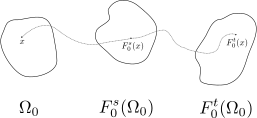
\includegraphics[width=\textwidth]{chp02_background/figures/flow_map.pdf}
% 		\caption{A pictorial representation of the flow map \(F\) corresponding to a continuous time dynamical system.
% 			An initial state \(x\) at time \(0\) is mapped to ..., illustrating the property \(F_s^t\!\left(F_0^s\!\left(x\right)\right) = F_0^t\!\left(x\right)\).}
% 		\label{fig:flow_map_diag}
% 	\end{center}
% \end{figure}


We use the flow map \(F\) to represent all solutions of the deterministic differential equation \cref{eqn:det_ode}, with the understanding that for any relevant initial condition, the flow map at that point can be readily computed by solving the ODE either analytically or numerically.

Moreover, the gradient of the flow map \(F\) (with respect to the initial condition) provides insight into the local behaviour of the dynamical system \citep{Arnold_1973_OrdinaryDifferentialEquations,TruesdellNoll_2004_NonLinearFieldTheories}.
For any times \(s, t \in [0,T]\), this gradient	\(\nabla F_s^t\) satisfies a useful property; the equation of variations.
\begin{equation}
	\dpd{\nabla F_{s}^{t}\!\left(x\right)}{t} = \nabla u\!\left(F_{s}^{t}\!\left(x\right), t\right) \nabla F_{s}^{t}\!\left(x\right).
	\label{eqn:eqn_of_variations}
\end{equation}
This result can be shown by taking the gradient of both sides in \eqref{eqn:flow_map_ode} and using the chain rule.







\subsection{Lagrangian coherent structures}\label{sec:bkg_lcs}
In this section, we have a brief sojourn into the field of Lagrangian coherent structures, which provide qualitative insight into the behaviour of a dynamical system, particularly in the fluid flow context.

In a steady system (that is, the vector field \(u\) in \cref{eqn:det_ode} is independent of time), we can gain this insight by using classical methods in dynamical systems, such as phase portrait analysis and identifying unstable and stable manifolds.
For example, unstable and stable manifolds cannot be intersected by solution trajectories, and so can act as barriers for the transport of material within a flow.
However, when the system is non-autonomous (that is, the vector field explicitly depends on time \(t\)), these structures can themselves vary with time and the problem of identifying them is far more non-trivial.
Lagrangian coherent structure (LCS) theory provides a mathematical framework for defining and identifying such structures within a given flow \citep{BalasuriyaEtAl_2018_GeneralizedLagrangianCoherent}.


\Cref{fig:lcs_examples} show examples of coherent structures in observed fluid flows, which can be considered LCSs.\lb{Get a proper reference. Photoplankton: \url{https://climate.nasa.gov/climate_resources/170/summer-blooms-in-the-baltic/}}

\begin{figure}
	\begin{center}
		\begin{subfigure}{0.49\textwidth}
			\caption{An oil slick from the \emph{Deepwater Horizon} oil spill in 2010.}
		\end{subfigure}
		\begin{subfigure}{0.49\textwidth}
			\includegraphics[width=\textwidth]{chp02_background/figures/red_spot.png}
			\caption{Jupiter's Great Red Spot, as photographed by the Voyager probe in 1979 (NASA/JPL-Caltech).}
		\end{subfigure}
		\begin{subfigure}{0.49\textwidth}
			\includegraphics[width=\textwidth]{chp02_background/figures/photoplankton}
			\caption{Photoplankton blooms in the Baltic sea.}
		\end{subfigure}

		\caption{Examples of coherent patterns emerging in fluid flows.}
		\label{fig:lcs_examples}
	\end{center}
\end{figure}


There are many procedures and heuristics for extracting these regions from a given flow, which draw upon
Detailed reviews of approaches to Lagrangian coherent structure extraction are provided by \citet{BalasuriyaEtAl_2018_GeneralizedLagrangianCoherent}, \citet{HadjighasemEtAl_2017_CriticalComparisonLagrangian}, and \citet{PeacockDabiri_2010_IntroductionFocusIssue}, for instance.

One of the best known procedures for extracting LCSs is via the finite-time Lyapunov exponent (FTLE) \citep{ShaddenEtAl_2005_DefinitionPropertiesLagrangian}, which is a measure quantifying the stretching of infinitesimal regions of a flow.


Take an initial condition \(x\) and let \(F_0^t\) represent the flow map of our dynamical system.
We wish to quantify the impact of a small change in the initial condition, so take \(\delta\) as a small and arbitrary perturbation to \(x\).
Then, we measure the \emph{stretching} in the direction of \(\delta\) with
\[
	s\!\left(x, \delta\right) = \frac{\norm{F_0^t\!\left(x + \delta\right) - F_0^t\!\left(x\right)}}{\norm{\delta}}
\]
For sufficiently small \(\delta\), we can replace the mapped perturbation with a linearisation of the flow map about \(x\), that is
\[
	s\!\left(x, \delta\right) \approx \frac{\norm{\nabla F_0^t\!\left(x\right) \delta}}{\norm{\delta}}.
\]
\Cref{fig:ftle_illustr} provides a pictorial representation of this calculation; a small !!!!!
Taking the supremum over all possible perturbations \(\delta\), we have
\[
	\sup_{\delta \in \R^n, \, \delta \neq 0}s\!\left(x, \delta\right) \approx \norm{\nabla F_0^t\!\left(x\right)},
\]
which quantifies the stretching about the trajectory \(F_0^t\!\left(x\right)\).
The finite-time Lyapunov exponent is then computed as
\begin{equation}
	\mathrm{FTLE}_0^t\!\left(x\right) = \frac{1}{\abs{t}}\ln\!\left(\norm{\nabla F_0^t\!\left(x\right)}\right).
	\label{eqn:ftle_defn}
\end{equation}
Note that the operator norm \(\norm{\nabla F_0^t\!\left(x\right)}\) in \cref{eqn:ftle_defn} can be readily computed as the square root of the largest eigenvalue of the Cauchy-Green tensor \(\left[\nabla F_0^t\!\left(x\right)\right]^{\T}\nabla F_0^t\!\left(x\right)\).

% In \Cref{fig:gs_lcs}, we compute the FTLE field of our Gulf Stream velocity model over a timespan of 7 days.



% \begin{figure}
% 	\begin{center}
% 		\begin{subfigure}{0.49\textwidth}
% 			\includegraphics[width=\textwidth]{chp02_background/figures/gulf_stream_motivation/ftle.pdf}
% 			\caption{The finite-time Lyapunov exponent field.}
% 		\end{subfigure}
% 		\begin{subfigure}{0.49\textwidth}
% 			\caption{Maximising ridges of the FTLE field.}
% 		\end{subfigure}
% 		\caption{The finite-time Lyapunov exponent field computed, and corresponding maximising ridges.
% 			This is an example of using a scalar field to extract Lagrangian coherent structures from a fluid flow.
% 			The resulting maximises ridges indicate a skeleton of the Gulf Stream.}
% 		\label{fig:gs_lcs}
% 	\end{center}
% \end{figure}


Most well-established LCS frameworks and extraction procedures are purely deterministic, in that they are defined and compute solely in terms of the dynamical system.
However, uncertainty in such dynamical systems is inevitable and these methods do not explicitly account for this.
There is therefore an emerging interest \citep{Balasuriya_2020_StochasticApproachesLagrangian} in extending LCS theory to stochastic settings (which is the relevance of LCSs to this thesis).
There are several different ways in which stochasticity is being accounted for in LCS frameworks:
\begin{romanate}
	\item in creating novel computable measures that explicitly account for such ongoing uncertainty, e.g. see stochastic sensitivity introduced by \citet{Balasuriya_2020_StochasticSensitivityComputable}, model sensitivity introduced by \citet{KaszasHaller_2020_UniversalUpperEstimate}, and the finite-time divergence rate by \citet{BranickiUda_2023_PathBasedDivergenceRates}.
	These are scalar fields defined on initial conditions that measure, and can be used to extract coherent regions in similar ways to deterministic methods.

	\item \citet{BalasuriyaGottwald_2018_EstimatingStableUnstable} consider stationary flows subject to small-scale stochastic perturbations, and quantify the behaviour of particles
	\citet{DennerEtAl_2016_ComputingCoherentSets} directly compute coherent sets by working with a discretised Fokker-Planck equation.

	\item in understanding the direct impact of velocity uncertainty on well-established deterministic LCS measures.
	\citet{BadzaEtAl_2023_HowSensitiveAre} provide a systematic analysis, using Monte Carlo simulation and summary statistics to evaluate the robustness of several common LCS extraction schemes to velocity uncertainty.
	It is shown that LCS methods that directly account for this uncertainty, such as stochastic sensitivity \citep{Balasuriya_2020_StochasticSensitivityComputable}, are the most robust.
	The finite-time Lyapunov exponent has received particular attention, with an initial study into the impac


\end{romanate}
In this thesis, we are primarily interested point (i), by exploring how our characterisations of uncertainty can be applied to extract coherent structures.
This is directly extending the stochastic sensitivity of \citet{Balasuriya_2020_StochasticSensitivityComputable}, which is summarised in \Cref{sec:s2_summ}.



\section{From ODEs to SDEs}
In practice, any differential equation model will be subject to unavoidable uncertainty, which can arise from a range of sources including but not limited to:
\begin{itemize}
	\item observational errors in any measured data used to construct the model,
	\item uncertainty in any parameters involved in the model,
	\item unexplainable phenomena not captured by the model,
	\item numerical errors in the discretisation of the model, and
	\item uncertainty in the knowledge of the initial state.
\end{itemize}

Since the true nature of this uncertainty is unknowable, it is common to model it as a random process.
That is, we extend our deterministic model to a stochastic one, where the solution (and therefore our predictions of the future state) is now a random variable.
There are several approaches to establishing such a framework, the most general of which is a random dynamical system \citep{Arnold_1998_RandomDynamicalSystems,NeckelRupp_2013_RandomDifferentialEquations}.
However, when working in a continuous-time and continuous-state modelling scenario, a natural extension of an ordinary differential equation to account for this uncertainty is a stochastic differential equation (SDE).
For a formal introduction to stochastic differential equations, see \citet{Oksendal_2003_StochasticDifferentialEquations} or \citet{KallianpurSundar_2014_StochasticAnalysisDiffusion}, for instance.
The following motivation of stochastic differential equations follows a similar one available in \citet{Oksendal_2003_StochasticDifferentialEquations}.

Suppose that we have a deterministic ordinary differential equation, i.e. \cref{eqn:ode_det}, and aim to account for uncertainty in the vector field \(u\).
In lieu of any additional understanding of this uncertainty, we model it as a stochastic noise.
Ideally, we would parameterise the uncertainty with some continuous-time stochastic process \(\xi_t\!\left(x_t\right)\), and write
\[
	\dod{y_t}{t} = u\left(x_t, t\right) + \xi_t\!\left(x_t\right).
\]
The noise process \(\xi_t\) can depend on the state, since we may expect that the magnitude and structure of the uncertainty varies with both the state and time.


Additionally, since we are modelling with a continuum, the noise process \(\xi_t\) should be (with probability \(1\)) continuous in time.
However, such a noise process \(\xi_t\) does not exist \citep{Oksendal_2003_StochasticDifferentialEquations}, in that there is no continuous process with properties 1 to 4, so we need an alternative formulation of the integral.
This leads to the It\^o integral, and It\^o stochastic differential equations, which we introduce in \Cref{sec:bkg_ito} and \Cref{sec:bkg_sde} respectively.



\subsection{The Wiener process}

The Wiener process, or Brownian motion, is an example of a continuous-time stochastic process that is often used to model \td{something}
In the absence of any additional knowledge about the nature of the noise (such as skew)
Defined formally, the (one-dimensional) \emph{Wiener process} is a stochastic process \(B_t\) taking values in \(\R\) and satisfying the following properties:
\begin{romanate}
	\item \(B_0 = 0\),
	\item for every \(s > 0\), the increments \(B_{s + t} - B_{s}\) for \(t \geq 0\) are independent of \(B_r\) for all \(r < s\),
	\item \(B_{s + t} - B_t \isGauss{0, s}\) for all \(s,t > 0\), and
	\item \(B_t\) is continuous in \(t\) almost surely.
\end{romanate}
Remarkably, these properties \emph{uniquely} define the Wiener process, with the additional result that for any \(t > 0\), \(B_t \sim \mathcal{N}\left(0, t\right)\), a Gaussian distribution with mean zero and variance \(t\).
The \emph{\(n\)-dimensional Wiener process} is a stochastic process \(W_t\) taking values in \(R^n\) such that each component of \(W_t\) is a one-dimensional Wiener process and the components of \(W_t\) are mutually independent.
It follows that for the \(n\)-dimensional Wiener process \(W_t\), at any time \(t > 0\), \(W_t \sim \mathcal{N}\left(0, tI\right)\), an \(n\)-dimensional Gaussian distribution with mean zero and covariance matrix \(tI\).

% A Wiener process is a type of L\'evy process, which is a more general class of stochastic process satisfying only conditions (i), (ii), and (iii) above \citep{Applebaum_2004_LevyProcessesStochastic}.

\Cref{fig:wiener_rels} plots realisations of a one-dimensional and two-dimensional Wiener process.

\begin{figure}
	\begin{center}
		\includegraphics[width=0.49\textwidth]{figures/wiener_realisations_1d.pdf}
		\includegraphics[width=0.49\textwidth]{figures/wiener_realisations_2d.pdf}
		\caption{(Left) Several realisations of a one-dimensional Wiener process \(W_t\) evolving through time, and (right) a realisation of two-dimensional Wiener process \(\left(W_t^{(1)}, W_t^{(2)}\right)\).}
		\label{fig:wiener_rels}
	\end{center}
\end{figure}


\subsection{The It\^o integral}\label{sec:bkg_ito}
\td{Some sort of motivation or introduction}
For our purposes, we can think of an It\^o integral as being defined as the limit in probability of a sequence of sums, i.e. for a scalar but possibly random-valued function \(f\colon [a,b] \to \R\),
\begin{equation}\label{eqn:ito_int_limit_defn}
	\sum_{\left[t_i, t_{i+1}\right] \in \mathcal{P}_N}{f\left(t_{i}\right)\left(W_{t_{i+1}} - W_{t_i}\right)} \xlongrightarrow[\text{probability}]{} \int_a^b{f(t)\dif W_t}, \quad \text{as } N \to \infty
\end{equation}
where \(\mathcal{P}_N\) is a partition of \(\left[a,b\right]\) with \(\lim_{N \to \infty}\mathcal{P}_N = [a,b]\), \emph{\`a la} the definition of the Riemann integral.
It can be shown (see the textbooks by \citet{KallianpurSundar_2014_StochasticAnalysisDiffusion} and \citet{Oksendal_2003_StochasticDifferentialEquations}, for instance) that this limit exists for a large class of both deterministic- and random-valued functions, by constructing appropriate approximations of the function \(f\).

The extension of the It\^o integral to vector- and matrix-valued functions is straightforward.
Let \(g \colon [a,b] \to \R^{n \times m}\) be a function giving possibly random \(n \times m\) matrices (take \(m = 1\) to describe a vector-valued function).
\begin{subequations}\label{eqn:mv_ito_defn}
	Then, we define the It\^o integral of \(g\) with respect to the \(m\)-dimensional Wiener process \(W_t\) over the time interval \([a,b]\) as
	\begin{equation}\label{eqn:mv_ito_defn_1}
		\int_a^b{g(t)\dif W_t} \coloneqq \left(\mathcal{I}_1, \dotsc, \mathcal{I}_n\right)^{\T},
	\end{equation}
	where
	\begin{equation}\label{eqn:mv_ito_defn_2}
		\mathcal{I}_{i} = \sum_{j=1}^m{\int_a^b{g_{ij}\left(t\right) \dif W_t^{(j)}}},
	\end{equation}
	for \(i = 1,\dotsc, n\) and where \(g_{ij}\) denotes the \((i,j)\)th element of \(g\).
\end{subequations}


\subsection{It\^o stochastic differential equations}\label{sec:bkg_sde}

The differential form of an \(n\)-dimensional It\^o stochastic differential equation is
\begin{equation}
	\dif y_t = u\!\left(y_t, t\right)\dif t + \sigma\!\left(y_t, t\right)\dif W_t,
	\label{eqn:gen_sde}
\end{equation}
where the solution \(y_t\) is a stochastic process taking values in \(\R^n\), \(u\colon \R^n \times \R \to \R^n\) is the drift and \(\sigma\colon \R^n \times \R \to \R^{n\times m}\) is the diffusivity.
The driving process \(W_t\) is the \(m\)-dimensional Wiener process.
The notation in \eqref{eqn:gen_sde} is not rigorously defined (the solution \(y_t\) is not differentiable in general, for example), but rather taken as equivalent to the integral form
\begin{equation}
	y_t = y_0 + \int_0^t{u\left(y_\tau, \tau\right)\dif\tau} + \int_0^t{\sigma\left(y_\tau, \tau\right)\dif W_\tau}.
	\label{eqn:gen_sde_int}
\end{equation}
where \(y_0\) is the possibly random initial condition.
In the most general case, the drift \(u\) and diffusivity \(\sigma\) are permitted to themselves be random functions\footnote{For more information, see for instance \citet{KallianpurSundar_2014_StochasticAnalysisDiffusion}.
	The formal treatment of such stochastic differential equations remains an area of open research, such as establishing the conditions for existence and uniqueness of solutions \citehere, and EXAMPLE.}, but in this thesis we assume that both are deterministic.

Stochastic differential equations also arise as the limit of deterministic slow-fast systems, where the average behaviour of the `fast' dynamics can be shown to converge to the solution of a stochastic differential equation \citep[e.g.]{WongZakai_1965_ConvergenceOrdinaryIntegrals,MelbourneStuart_2011_NoteDiffusionLimits,GottwaldMelbourne_2013_HomogenizationDeterministicMaps}\lb{Maybe some better citations out there.}.
A review of this theory is provided by \citet{GivonEtAl_2004_ExtractingMacroscopicDynamics}.
This is particular relevant in climate and physics applications, where \citep{FranzkeEtAl_2015_StochasticClimateTheory}.
This leads to stochastic parameterisation \citep{BernerEtAl_2017_StochasticParameterizationNew,Palmer_2019_StochasticWeatherClimate}, which we review in more detail in \Cref{sec:stoch_param}.




\subsection{Numerical schemes for approximating SDEs}
In general, solving a stochastic differential equation analytically is not possible, and so as with ordinary differential equations we instead look to use numerical schemes to approximate solutions.
However, the solution to a stochastic differential equation is itself a random variable, so a single sample path is not sufficient.
Instead, a numerical SDE scheme produces approximate \emph{realisations} of the solution.
The Euler-Maruyama (EM) method is analogous to the Euler method for ODEs, and considered by many to be the simplest method for numerically solving SDEs \citep{KloedenPlaten_1992_NumericalSolutionStochastic}.
The update step of the EM scheme, with step size \(\Delta t\), is
\begin{equation}
	\hat{x}_{t + \Delta t} = \hat{x}_{t} + \Delta t u\left(\hat{x}_t, t\right) + \Delta t \sigma\left(\hat{x}_t, t\right) Z_t,
	\label{eqn:em_step}
\end{equation}
where \(Z_t\) is sampled from the standard Gaussian \(\Gauss{0,I}\), and the scheme is initialised as \(\hat{x}_0 = x_0\).
The Euler-Maruyama scheme has strong order 0.5, meaning that
\[
	\avg{\norm{x_t - \hat{x}_{t}\left(\Delta t\right)}} = \mathcal{O}\left(\Delta t^{0.5}\right),
\]
where \(\hat{x}_t\left(\Delta t\right)\) is the Euler-Maruyama estimate at time \(t\) using step size \(\Delta t\).


There are many other schemes for generating approximate samples of a stochastic differential equation, of varying weak and strong orders.
For instance, extensions of Runge-Kutta-type schemes \citep{Roberts_2012_ModifyImprovedEuler,Rossler_2010_RungeKuttaMethodsStrong}.






\subsection{The Fokker-Planck equation}\label{sec:fp_eqn}
The probability density function \(\rho: \R^n \times [0,T] \to [0,\infty)\) for the solution to \eqref{eqn:gen_sde} at time \(t \in [0,T]\) is the solution to the corresponding Fokker-Planck equation \citep{Risken_2012_FokkerPlanckEquationMethods}
\begin{equation}
	\dpd{\rho}{t} = \frac12\nabla\cdot\nabla\cdot\left(\rho\sigma\sigma^{\T}\right) - \nabla\cdot\left(\rho u\right)
	\label{eqn:fp_eqn}
\end{equation}
subject to some initial density \(\rho\left(x,0\right)\) given by the initial condition to \eqref{eqn:gen_sde}.
To ensure that the solution is a valid probability density function on \(\R^n\), for any \(t \in [0,T]\), \(\rho\) must satisfy
\begin{subequations}\label{eqn:fp_valid_pdf}
	\begin{align}
		\int_{\R^n}{\rho\left(x, t\right)\dif x} = 1, \label{eqn:fp_valid_pdf_norm} \\
		\lim_{x \to \infty}\rho\left(x,t\right) = 0. \label{eqn:fp_valid_pdf_limit}
	\end{align}
\end{subequations}
For a fixed and deterministic initial condition \(y_0 = x\), the corresponding initial condition to \eqref{eqn:fp_eqn} is the Dirac-delta distribution centred at \(x\).


\subsubsection{Relationship to the classical advection-diffusion equation}
The advection-diffusion equation describes the time-evolution of a passive and inert scalar quantity, such as temperature, salinity

\citep{Visser_2008_LagrangianModellingPlankton}

Let \(c \colon \Omega_0 \times [0,T] \to [0, \infty)\) denote the concentration of a passive and inert scalar quantity, then the classical advection-diffusion equation is
\begin{equation}\label{eqn:advec_diff}
	\dpd{c}{t} = - \nabla\cdot \left(v\!\left(x,t\right)c\!\left(x,t\right)\right) + \nabla\cdot\left(K\!\left(x,t\right)\nabla c\!\left(x,t\right)\right), \quad c\!\left(x,0\right) = c_0\!\left(x\right),
\end{equation}
where \(v\) denotes the flow velocity dictating the advection (displacement) of the tracer, and \(K\) is a matrix describing the diffusion (dispersion) of \(c\).




If we set \(u\!\left(x,t\right) = v\!\left(x,t\right) + \nabla \cdot K\!\left(x,t\right)\) and \(\sigma\!\left(x,t\right)\sigma\!\left(x,t\right) = K\!\left(x,t\right)\), then the Fokker-Planck equation \cref{eqn:fp_eqn} is equivalent to the advection-diffusion equation \eqref{eqn:advec_diff}.
Thus, the evolution of the tracer concentration under \cref{eqn:advec_diff} can be equivalently considered as the probability density function of solutions to the stochastic differential equation
\begin{equation}\label{eqn:ad_sde}
	\dif x_t = \left[u\!\left(x_t, t\right) + \nabla \cdot K\!\left(x_t, t\right)\right]\dif t + \kappa\!\left(x_t, t\right)\dif W_t, \quad x_t \sim \hat{c}_0,
\end{equation}
where \(\kappa\) is any matrix-valued function satisfying \(K \equiv \kappa\kappa^{\T}\), and
\[
	\hat{c}_0\!\left(x\right) = \frac{c_0\!\left(x\right)}{\int_{\Omega_0}c_0\!\left(z\right)\dif z},
\]
is the initial density of \eqref{eqn:advec_diff} normalised to describe a probability density function.
Assuming that the total concentration tracer is conserved, that is
\[
	\int_{\Omega_t}{c\!\left(z,t\right)\dif z} = \int_{\Omega_0}{c_0\!\left(z\right)\dif t}
\]
for all \(t \in [0,T]\), then we can recover \(c\) from the probability density function \(\rho\) corresponding to \cref{eqn:ad_sde} as
\[
	c\!\left(x,t\right) = \rho\!\left(x,t\right)\int_{\Omega_0}{c_0\!\left(z\right)\dif t}.
\]
An implication of this connection is that the theory and computations for stochastic differential equations developed throughout this thesis can be applied to \emph{any} scalar field that is modelled with an advection-diffusion type equation.



\subsubsection{Practical difficulties}

However, there are several practical difficulties with using the Fokker-Planck equation:
\begin{itemize}
	\item \textbf{Dimensionality:}
	\item \textbf{Boundary conditions:}
\end{itemize}



\subsubsection{Green's function method}
The Fokker-Planck equation is linear, so we can apply a technique known as Green's function method (for an example of this approach on a linear SDE, see Section 3.2 of \citet{Risken_2012_FokkerPlanckEquationMethods}) in order to understand the behaviour of solutions with non-fixed initial conditions.
Let \(\mathcal{P}_t\set{\rho_0}\) denote the solution operator of \eqref{eqn:fp_eqn} with initial density \(\rho_0\colon \R^n \to \R^n\).
Then, since \eqref{eqn:fp_eqn} is a linear equation, \(\mathcal{P}_t\) is a linear operator.
Now, let \(x_0 \in \R^n\) be an arbitrary fixed point, and consider the fundamental solution, or Green's function,
\[
	G_t\left(x; x_0\right) \coloneqq \mathcal{P}_t\set{\delta_{x_0}}\!\left(x\right).
\]
That is, \(G_t\left(x; x_0\right)\) is the solution to the Fokker-Planck equation with the Dirac-delta initial condition \(\delta_{x_0}(x) = \delta\left(x - x_0\right)\), which is equivalent to the SDE \eqref{eqn:gen_sde} with the deterministic and fixed initial condition \(y_0 = x_0\).
The Green's function \(G_t\) is equivalently the transition probability function of the SDE solution \(x_t\) as a stochastic process.
Now, using the sampling property of the Dirac-delta function, for a general initial density \(\rho_0\colon \R^n \to \R^n\),
\[
	\rho_0(x_0) = \int_{\R^n}{\rho_0\left(x\right)\delta_{x_0}\left(x\right)\dif x}.
\]
Since \(\mathcal{P}_t\) is linear,
\begin{equation}
	\mathcal{P}_t\set{\rho_0}\!\left(x_0\right) = \int_{\R^n}{\rho_0\!\left(x\right)\mathcal{P}_t\set{\delta_{x_0}}\!\left(x\right)\dif x} = \int_{\R^n}{\rho_0\!\left(x\right) G_t\!\left(x; x_0\right)\dif x}.
	\label{eqn:fp_greens_trick}
\end{equation}



\section{Stochastic parameterisation}\label{sec:stoch_param}

Many numerical weather and climate prediction models rely upon a spatial discretisation for tractable analysis and simulation.
Often, an extremely high resolution is needed to produce accurate simulations and predictions; for example, \citet{DawsonEtAl_2012_SimulatingRegimeStructures} demonstrated such requirements\lb{Read paper and be specific about numbers} for the state-of-the-art European Centre for Medium-Range Weather Forecasts (ECMWF) forecast model.

The formal introduction of stochastic terms to account for unknown and unresolved processes into an otherwise deterministic model is known as \emph{stochastic parameterisation}, particularly in scientific circles.
\citet{BernerEtAl_2017_StochasticParameterizationNew} review the need for stochastic parameterisation in weather and climate models and discuss how stochastic terms can quantify four different aspects of these models:
\begin{itemize}
	\item directly estimating uncertainty,
	\item reducing systematic model errors arising from unresolved subgrid processes,
	\item triggering regime changes, and
	\item encapsulating the effect of external forcing.
\end{itemize}


\begin{figure}
	\begin{center}
		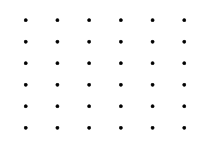
\includegraphics[width=\textwidth]{chp02_background/figures/gridpoints.pdf}
		\caption{An illustration of unresolved subgrid effects in a spatial discretisation.
			When a system is discretised, either from measurements or to numerically solve a model, processes between the grid points and no longer resolved or observed and yet can have a noticeable impact on the system.}
		\label{fig:subgrid_effects}
	\end{center}
\end{figure}


In particular, \citet{SuraEtAl_2005_MultiplicativeNoiseNonGaussianity} demonstrate that linear deterministic dynamics with multiplicative noise can be produce the non-Gaussian statistics that we observed in real systems.

\citet{DawsonPalmer_2015_SimulatingWeatherRegimes} showed through simulation studies that the performance of a high-resolution purely deterministic model can be matched by a lower-resolution stochastic model.


The mathematical formulation of stochastic parameterisation -- where model predictions are now random quantities -- lends itself naturally to data assimilation \citep{BudhirajaEtAl_2019_AssimilatingDataModels,Jazwinski_2014_StochasticProcessesFiltering,LawEtAl_2015_DataAssimilationMathematical,ReichCotter_2015_ProbabilisticForecastingBayesian}, where ongoing observations are combined with predictions from a model to produce an improved forecast.
Data assimilation provides a framework that can simultaneously account for uncertainty in the observations and the model itself.
It has been shown that stochastic parameterisation can improve the quality of forecasts in data assimilation schemes \citep{MitchellGottwald_2012_DataAssimilationSlow,HaEtAl_2015_ComparisonModelError}, and so these applications are an active error of research \citep[e.g.]{GottwaldHarlim_2013_RoleAdditiveMultiplicative}.

\td{Flow from here into the need for maths - justifications, proofs, etc.?}
There is an emerging need to bridge the gap between mathematicians working on developing stochastic theory and algorithms, and the scientists looking to apply this work to their respective fields.
In particular, \citet{BernerEtAl_2017_StochasticParameterizationNew} conclude that ``geoscientists are often unaware of mathematically rigorous results that can aid in the development of physically relevant parameterizations, [while] mathematicians often do not know about open issues in scientific applications that might be mathematically tractable''.


Although stochastic parameterisation is more common in the atmospheric modelling context, oceanography also suffers from the same trade-off between spatial resolution and accuracy of predictions.

In the context of a fluid, unresolved processes can be vortices, eddies and turbulence \citep{Griffa_1996_ApplicationsStochasticParticle}.

The mixing effect that these eddies have on the surrounding flow can be modelled with spatiotemporally-varying diffusion \citehere, which via the Fokker-Planck equation can be equivalently formulated as a stochastic differential equation with multiplicative noise.
The Lagrangian trajectories, incorporating these unresolved eddy effects, are then modelled as solutions to the stochastic differential equation.
Equivalently, through the Fokker-Planck equation we can consider the evolution of a passive tracer undergoing advection due to the deterministic drift and diffusion from both any natural diffusivity and the unresolved processes.
The probability density function that solves the Fokker-Planck equation can be instead thought of as a time-varying density (with the appropriate normalisation) of the tracer.
For instance, the Fokker-Planck equation has been used to model the transport of ??? with a stochastic framework \citehere.
Hence, understanding the evolution of solutions to a stochastic differential equation is valuable in oceanography, as a means of quantifying both observational error and unresolved subgrid processes.


There are several different methods for quantifying eddy diffusivity given either observed tracer data or a global ocean circulation model.

The simplest notion of eddy diffusivity is a defined by






A recent approach by \cite{YingEtAl_2019_BayesianInferenceOcean} uses Bayesian inference to estimate the eddy diffusivity tensor from observed Lagrangian tracer data, by numerically solving the Fokker-Planck equation to compute a likelihood function.


In summary, stochastic parameterisation



\section{Limitations of stochastic simulation and the need for further development}\label{sec:bkg_sim_limits}
The introduction of stochastic terms complicates both the analytical treatment of the model.
For example, we saw in \Cref{sec:sde_theory} that adding even additive and stationary\lb{Is this the right word?? I mean that \(\sigma\) is constant, with no time-dependency}\td{need to define additive versus multiplicative properly.} noise to an analytically solvable non-linear deterministic model can make exact solutions intractable.
Thus, across many applications the state of the art approach is to generate samples of the stochastic model and perform statistical inference.
For example, Monte-Carlo simulation is used across weather forecasting \citep{LeutbecherEtAl_2017_StochasticRepresentationsModel}, \td{something atmospheric} and \td{something oceanic}.

However, the most significant drawback of bulk stochastic simulation is the computational load.
In general, a large number of samples is required for convergent statistics and accurate inference, as discussed by \citet{Leutbecher_2019_EnsembleSizeHow}.
For a complex model, the computational load of computing a single realisation

The recent review by \citet{LeutbecherEtAl_2017_StochasticRepresentationsModel} highlights the need to develop computationally efficient schemes for quantifying stochasticity in weather and climate forecast models.


\td{Show the plateauing out that I am observing empirically when using a KDE . . . some literature on this?? This is a huge point to make}
For example, suppose that we intend on using the probabilistic forecast of our stochastic model in an inference scheme, such as in data assimilation in which model predictions are combined with ongoing observations to produce an improved forecast \cite[e.g.]{LawEtAl_2015_DataAssimilationMathematical,BudhirajaEtAl_2019_AssimilatingDataModels, ReichCotter_2015_ProbabilisticForecastingBayesian}.
This requires a probability density function or similar for our forecast, but in generating samples we initially only have a collection of finite discrete points.


The overall aim of this thesis is to address this problem, by developing characterisations of uncertainty and algorithms for approximating solution probability densities (as opposed to just generating samples) that are computationally efficient.
We aim to take advantage of the computational ease of generating solutions to a deterministic system (relative to taking many samples of a stochastic one).


The purpose of this example was to highlight the importance of accounting for measurement error and unresolved processes in a ; when the dynamics are complicated, then any uncertainty can have a significant impact on our inferences from the model, both quantitatively and qualitatively.



\section{Stochastic sensitivity}\label{sec:s2_summ}
To conclude our background and motivation, this section provides a brief summary of stochastic sensitivity, as introduced by \citet{Balasuriya_2020_StochasticSensitivityComputable} as a means of quantifying uncertainty
Further technical details, including the main theorems, are reproduced in \Cref{app:s2_details}.

Given possibly time-dependent velocity data \(u: \R^2 \times [0,T] \to \R^2\), \citet{Balasuriya_2020_StochasticSensitivityComputable} considers the evolution of solutions to the differential equation
\[
	\dod{x_t}{t} = u\left(x_t, t\right).
\]
Solutions can be summarised by the flow map \(F_{t_1}^{t_2}\), as in \Cref{def:flow_map}.
In most practical situations, the Eulerian velocity data driving ocean and atmospheric models relies upon measurements of estimates obtained on a low resolution spatial discretisation.
\citet{Balasuriya_2020_StochasticSensitivityComputable} introduces stochastic sensitivity as a new tool for directly quantifying the impact of Eulerian uncertainty on Lagrangian trajectories.
The evolution of Lagrangian trajectories is modelled as solution to a It\^o stochastic ordinary differential equation.

To directly account for these unresolved sources of uncertainty, the ``true'' Lagrangian trajectories evolve as solution to the stochastic differential equation
\begin{equation}
	\sde{y_t}{u\left(y_t, t\right)}{\epsilon\sigma\left(y_t, t\right)},
	\label{eqn:ss_sde},
\end{equation}
where \(0 < \epsilon \ll 1\) is a parameter quantifying the scale of the noise, \(\sigma:	\R^2\times[0,T] \to \R^{2\times 2}\) is the \(2\times 2\) diffusion matrix, and \(W_t\) is the canonical two-dimensional Wiener process.
In the original formulation \citep{Balasuriya_2020_StochasticSensitivityComputable}, \(\epsilon\) is a dimensionless parameter and \(\sigma\) is dimensional, but an alternative scaling technique relates \(\epsilon\) to spatial and velocity uncertainty scales in the data (see the follow-up work by \citet{BadzaEtAl_2023_HowSensitiveAre,Balasuriya_2020_UncertaintyFinitetimeLyapunov,FangEtAl_2020_DisentanglingResolutionPrecision})
Since \(\sigma\) can vary by both space and time, the noise is multiplicative.
The diffusion matrix \(\sigma\) is specified \emph{a priori}, based on any knowledge of how uncertainty varies with space and time, e.g. from experimental considerations, observation error estimates.
If no such prior information is known, then \(\sigma \equiv I\), the \(2 \times 2\) identity matrix is the default choice.

To quantify uncertainty in a way that is independent of the noise scale \(\epsilon\), \citet{Balasuriya_2020_StochasticSensitivityComputable} defined the random variable \(z_\epsilon\left(x,t\right)\) on \(\R^2 \times [0,T]\) as
\[
	z_\epsilon\left(x,t\right) \coloneqq \frac{y_t - F_0^t(x)}{\epsilon}.
\]
The main aim is to compute statistics of \(z_\epsilon\) at the final time \(T\), so that of \(z_\epsilon\left(x,T\right)\).
\citet{Balasuriya_2020_StochasticSensitivityComputable} then considers the signed projection of \(z_\epsilon\left(x,T\right)\) onto a ray emanating from the deterministic position \(F_0^T(x)\) in a given direction, defining
\[
	P_\epsilon\left(x,\theta\right) \coloneqq \hat{n}^{\T} z_\epsilon(x,T),
\]
where \(\theta \in \left[-\pi/2, \pi/2\right)\) and
\[
	\hat{n}(\theta) = \begin{bmatrix}
		\cos{\theta} \\
		\sin{\theta}
	\end{bmatrix}.
\]

The statistics of \(z_\epsilon\left(x,T\right)\) and \(P_\epsilon(x,\theta)\) are considered in the limit as \(\epsilon\downarrow 0\), which provides a characterisation of the uncertainty of the model \emph{independently} of the scale of the noise.
\citet{Balasuriya_2020_StochasticSensitivityComputable} provided computable expressions for the mean and variance of \(P_\epsilon\left(x,\theta\right)\) in this limit of small noise, which we summarise here.
For proofs of these results, see the appendices of \citet{Balasuriya_2020_StochasticSensitivityComputable}.

\begin{definition}[\citealt{Balasuriya_2020_StochasticSensitivityComputable}]
	\begin{alpharate}
		\item The \textbf{anisotropic uncertainty} is a scalar field \(A: \R^2\times\left[-\pi/2, \pi/2\right) \to [0,\infty)\) defined by
		\[
			A(x,\theta) \coloneqq \sqrt{\lim_{\epsilon\downarrow 0}\var{P_\epsilon(x,\theta)}}.
		\]

		\item The \textbf{stochastic sensitivity} is a scalar field \(S: \R^2 \to [0,\infty)\) defined by
		\[
			S^2(x) \coloneqq \lim_{\epsilon\downarrow 0}\sup_{\theta}{\var{P_\epsilon(x,\theta)}}.
		\]
	\end{alpharate}
\end{definition}

By employing techniques from both deterministic and stochastic calculus (i.e. Gr\"onwall's inequality, the Burkholder-Davis-Gundy inequality, It\^o's Lemma), Balasuriya further established expressions for both the anisotropic uncertainty and the stochastic sensitivity that are computable given only the flow map and velocity data.

\begin{theorem}[\citealt{Balasuriya_2020_StochasticSensitivityComputable}]\label{thm:orig_s2_calculation}
	For \(x \in \R^2\), set \(w \coloneqq F_0^t(x)\).
	Then, for any \(\theta \in \left[-\pi/2, \pi/2\right)\),
	\[
		A(x,\theta) = \left(\int_0^T{\norm{\Lambda\left(x, t, T\right)J\hat{n}(\theta)}\dif t}\right)^{1/2},
	\]
	where
	\[
		\Lambda\left(x,t,T\right) \coloneqq e^{\int_t^T{\left[\nabla \cdot u\right]\left(F_0^\xi(x), \xi\right)\dif\xi}}\sigma\left(F_0^t(x), t\right)^{\T}J \nabla_w F_T^t\left(w\right),
	\]
	with the gradients \(\nabla_w\) of the flow map taken with respect to the mapped position \(w\), and
	\[
		J \coloneqq \begin{bmatrix}
			0 & -1 \\
			1 & 0
		\end{bmatrix}
	\]
	Additionally, stochastic sensitivity is computed as
	\[
		S^2(x) = P(x) + N(x),
	\]
	with
	\begin{align*}
		L(x) & \coloneqq \frac12\sum_{i=1}^2\int_0^T\left[\Lambda_{i2}\left(x,t, T\right)^2 - \Lambda_{i1}\left(x,t,T\right)^2\right]\dif t \\
		M(x) & \coloneqq \sum_{i=1}^2\int_0^T{\Lambda_{i1}\left(x,t,T\right)\Lambda_{i2}\left(x,t,T\right)\dif t}                           \\
		N(x) & \coloneqq \sqrt{L^2(x) + M^2(x)}                                                                                             \\
		P(x) & \coloneqq \abs{\frac12\sum_{i=1}^2\sum_{j=1}^2{\int_0^T{\Lambda_{ij}\left(x,t,T\right)^2\dif t}}},
	\end{align*}
	where \(\Lambda_{ij}\) is the \((i,j)\)-element of \(\Lambda\).
\end{theorem}





\subsection{Current applications \& shortcomings}
Since stochastic sensitivity is only a recent development, it has only been applied in a limited number of places so far.
Here, we briefly review the literature in which the original formulation stochastic sensitivity by \citet{Balasuriya_2020_StochasticSensitivityComputable} has been applied.

\begin{itemize}
	\item \citet{Balasuriya_2020_UncertaintyFinitetimeLyapunov} uses stochastic sensitivity to compute an error bound for the finite-time Lyapunov (FTLE) computation.
	      The computable \(S^2\) value is used as an estimate of the standard deviation of the deviation between the deterministic and ``true'' (stochastic) trajectories, leading to a computable error bound on the FTLE value.


	\item \citet{FangEtAl_2020_DisentanglingResolutionPrecision}


	\item \citet{BadzaEtAl_2023_HowSensitiveAre} investigate the impact of velocity uncertainty on Lagrangian coherent structures (e.g. see the reviews by \citet{BalasuriyaEtAl_2018_GeneralizedLagrangianCoherent} and \citet{HadjighasemEtAl_2017_CriticalComparisonLagrangian}) extracted as robust sets with stochastic sensitivity.
	      The stochastic model \cref{eqn:ss_sde} is used to generate realisations of Lagrangian trajectories subject to noise on the velocity field.
	      By directly capturing such uncertainty as a means of coherent set \citet{BadzaEtAl_2023_HowSensitiveAre} showed that robust sets extracted with stochastic sensitivity do SOMETHING.

\end{itemize}
There are several limitations to the work as originally presented by \citet{Balasuriya_2020_StochasticSensitivityComputable}:
\begin{enumerate}
	\item The tools are restricted to two-dimensional models, and the constructions using projections have no obvious extension to \(n\)-dimensions.
	      Extending stochastic sensitivity to \(n\)-dimensions will enable application to a much broader class of models beyond the fluid flow context, including high-dimensional climate models.

	\item \citet{Balasuriya_2020_StochasticSensitivityComputable} only computes the expectation and variance of the projections \(P_\epsilon(x,\theta)\), which does not give us the distribution under the limit as \(\epsilon\) approaches 0.

	\item The computational formula for the anisotropic uncertainty and stochastic sensitivity, as described in \Cref{thm:orig_s2_calculation}, require knowledge of the divergence \(\nabla\cdot u\) of the velocity field, and computation of four integrals.
\end{enumerate}



In \Cref{sec:theory_s2}, we present an extension of stochastic sensitivity to \(n\)-dimensions that overcomes these limitations.

\chapter{Characterising SDE linearisations: the theory}\label{ch:linear_theory}
In general, stochastic differential equations cannot be solved analytically and instead require numerical simulations.
However, as we highlighted in \Cref{sec:bkg_sim_limits} there are limitations to relying upon these bulk simulations, such as computational expense.
An alternative approach is to approximate the SDE by a simplified one, which can be solved analytically.
A linearisation procedure is one such approach when the noise is small, which replaces the coefficients of the SDE with first-order Taylor expansions.
This linearisation scheme is accordingly used across a range of literature and applications \citep{Jazwinski_2014_StochasticProcessesFiltering,SarkkaSolin_2019_AppliedStochasticDifferential,KaszasHaller_2020_UniversalUpperEstimate,ArchambeauEtAl_2007_GaussianProcessApproximations,Sanz-AlonsoStuart_2017_GaussianApproximationsSmall,LawEtAl_2015_DataAssimilationMathematical,ReichCotter_2015_ProbabilisticForecastingBayesian,BudhirajaEtAl_2019_AssimilatingDataModels,LeGlandWang_2002_AsymptoticNormalityPartially}.

In this chapter, we build upon previous small-noise studies by \citet{Blagoveshchenskii_1962_DiffusionProcessesDepending}, \citet{FreidlinWentzell_1998_RandomPerturbationsDynamical}, and \citet{Sanz-AlonsoStuart_2017_GaussianApproximationsSmall} to provide an explicit bound for the error between a general class of stochastic differential equations and corresponding computable linearisations written in terms of a deterministic system.
Our framework accounts for non-autonomous coefficients, multiplicative noise, and uncertain initial conditions.
In \Cref{sec:theory}, we state the bound, written in terms of both the initial and the ongoing uncertainty, and provide an explicit characterisation of the solution to the linearised SDE including computations for the first two moments.

The second contribution of this chapter is to provide theoretical and computational extension to the original formulation of stochastic sensitivity by \citet{Balasuriya_2020_StochasticSensitivityComputable}, in \Cref{sec:theory_s2}.
We provide a definition of stochastic sensitivity for \(n\)-dimensions, and establish that the value can be computed from a linearised SDE.


Much of the content in this chapter and the following (\Cref{ch:linear_numerics}) has been submitted as a research article to \textit{Communications in Mathematical Sciences} \citep{BlakeEtAl_2023_ConvergenceStochasticDifferential}, and is currently under review.
The preprint is available on arXiv at \href{https://arxiv.org/abs/2309.16334}{arXiv:2309.16334}.
\Cref{sec:ftle_s2_connection}, which discusses the connections between stochastic sensitivity and the finite-time Lyapunov exponent, does not appear in the submitted article, and is instead a new contribution in this thesis.


\section{Convergence of a SDE to a linearisation}\label{sec:theory}
Suppose we are interested in the evolution of a \(\R^n\)-valued state variable \(y_t\) over a finite time interval \([0,T]\).
Our model, accounting for uncertainties arising from a range of sources, for the evolution of this variable is the It\^o stochastic differential equation
\begin{equation}
	\dif y_t^{(\epsilon)} = u\!\left(y_t^{(\epsilon)}, t\right)\dif t + \epsilon \, \sigma\!\left(y_t^{(\epsilon)}, t\right)\dif W_t, \quad y_0^{(\epsilon)} = x
	\label{eqn:sde_y}
\end{equation}
where \(u\colon \R^n \times [0,T] \to \R^n\) is the governing reference vector field.
The canonical \(m\)-dimensional Wiener process \(W_t\)  is a continuous white-noise stochastic process with independent Gaussian increments.
The scale of the ongoing noise is assumed to be small and is parameterised as \(0 < \epsilon \ll 1\).
The noise in \cref{eqn:sde_y} is multiplicative, in that the diffusion matrix \(\sigma\colon \R^n \times [0,T] \to \R^{n\times m}\) can vary with state \( x \), as well as with time \( t \).
We assume that \(\sigma\) is specified \textit{a priori}, or if no such information is known, then \(\sigma \equiv I\), the \(n \times m\) identity matrix, is a default modelling choice.
We consider \cref{eqn:sde_y} subject to the \emph{general} uncertain initial condition \(y_0^{(\epsilon)} = x\), where \(x\) is an \(n\)-dimensional random vector with some given distribution. The two sources of randomness, $ x $ and $ W_t $, are assumed independent from each other.

In the absence of any uncertainty (i.e. \(\epsilon = 0\) and the initial condition is a known deterministic quantity), \cref{eqn:sde_y} reduces to the ordinary differential equation
\begin{equation}
	\dod{y_t^{(0)}}{t} = u\!\left(y_t^{(0)}, t\right), \quad y_0^{(0)} = x_0.
	\label{eqn:ode_det}
\end{equation}
where the initial condition \(x_0 \in \R^n\) is fixed.
The formal convergence of the stochastic solution \(y_t^{(\epsilon)}\) (under certain conditions on the initial condition) to the deterministic \(y_{t}^{(0)}\) in the limit as \(\epsilon \to 0\) is well-established using the large deviations principle \citep[e.g]{FreidlinWentzell_1998_RandomPerturbationsDynamical}.
We refer to \cref{eqn:ode_det} as the \emph{reference} deterministic model associated with \cref{eqn:sde_y}.
Solutions to the reference deterministic model are more readily available, e.g. in terms of computational efficiency when solving numerically, than those of the stochastic model, but do not account for inevitable uncertainty.

Let the flow map \(F_{0}^{t}\colon \R^n \to \R^n\) be the function which evolves an initial condition from time \(0\) to time \(t\) according to the flow of \cref{eqn:ode_det}, i.e. \(F_0^t\!\left(x_0\right) = y_t^{(0)}\).

We assume certain smoothness and boundedness conditions on the various terms outlined, which are stated explicitly in \Cref{hyp:smooth}.
Throughout this article, we use the norm symbol \(\norm{\cdot}\) to denote (i) for a vector, the standard Euclidean vector norm, (ii) for a matrix, the spectral norm induced by the Euclidean norm, and (iii) for a 3rd-order tensor, the spectral norm induced by the matrix norm.
The gradient symbol \(\nabla\) generically refers to derivatives with respect to the state variable.

\renewcommand\thehypo{H}
\begin{hypo}\label{hyp:smooth}
	Let the deterministic functions \(u \colon \R^n\times [0,T] \to \R^n\) and \(\sigma \colon \R^n \times [0,T] \to \R^{n\times m}\), and the random initial condition \(x\) be such that:
	\begin{enumerate}[label=(H.\arabic{*}), ref=H.\arabic{*}]
		\item\label{hyp:fm_exists} For all \(t \in [0,T]\) flow map \(F_0^t \colon \R^n \to \R^n\) is well-defined, and continuously differentiable (with respect to the initial condition) with invertible derivative.

		\item\label{hyp:coef_cont} For each \(t \in [0,T]\), the function \(u(\cdot, t): \R^n \to \R^n\) given by \(u(x,t)\) is twice continuously differentiable on \(\R^n\), and each component of the function \(\sigma(\cdot, t): \R^n \to \R^{n\times m}\) given by \(\sigma(x,t)\) is differentiable on \(\R^n\).

		\item\label{hyp:u_bounds} There exists a constant \(K_{\nabla u} \geq 0\) such that for any \(t \in [0,T]\) and \(x \in \R^n\),
		\begin{equation*}
			\norm{\nabla u(x,t)} \leq K_{\nabla u}.
		\end{equation*}
		Equivalently, for all \(t \in [0,T]\), the function \(u\!\left(\cdot, t\right)\) is Lipschitz continuous with Lipschitz constant \(K_{\nabla u}\).

		\item\label{hyp:coef_meas} For each \(x \in \R^n\), the function \(u(x,\cdot) \coloneqq [0,T] \to \R^n\) and each component of the function \(\sigma(x,\cdot) \coloneqq [0,T] \to \R^{n\times m}\) are Borel-measurable on \([0,T]\).

		\item\label{hyp:linear_growth} There exists a constant \(K_L\) such that for any \(t \in [0,T]\) and \(x \in \R^n\),
		\[
			\norm{u\left(x,t\right)} + \norm{\sigma\left(x,t\right)} \leq K_L\left(1 + \norm{x}\right).
		\]

		\item\label{hyp:sigma_deriv_bound} There exists a constant \(K_{\nabla\sigma} \geq 0\) such that for any \(t \in [0,T]\) and \(x \in \R^n\),
		\begin{equation*}
			\norm{\nabla\sigma(x,t)} \leq K_{\nabla\sigma},
		\end{equation*}
		and we take \(K_{\nabla\sigma} = 0\) if there is no spatial dependence in \(\sigma\).
		Equivalently, for all \(t \in [0,T]\), the function \(\sigma\!\left(x, \cdot\right)\) is Lipschitz continuous with Lipschitz constant \(K_{\nabla\sigma}\).

		\item\label{hyp:init_indep} The initial condition \(x\) is defined on the same probability space as \(W_t\), and is independent of \(W_t\) for all \(t \in [0,T]\).

		\item\label{hyp:nnu_bounds} There exists a constant \(K_{\nabla\nabla u} \geq 0\) such that for any \(t \in [0,T]\) and \(x \in \R^n\),
		\[
			\norm{\nabla \nabla u(x,t)} \leq K_{\nabla\nabla u},
		\]
		and we take \(K_{\nabla\nabla} = 0\) if the second spatial derivatives of \(u\) are all zero.

		\item\label{hyp:sigma_bounds} There exists a constant \(K_\sigma \geq 0\) such that for any \(t \in [0,T]\) and \(x \in \R^n\),
		\begin{equation*}
			\norm{\sigma(x,t)} \leq K_{\sigma}.
		\end{equation*}

	\end{enumerate}
\end{hypo}
The conditions \ref{hyp:coef_cont} to \ref{hyp:init_indep} guarantee that \cref{eqn:sde_y} with the initial condition \(y_0 = x\) has a unique strong solution \citep{KallianpurSundar_2014_StochasticAnalysisDiffusion}.
The bound \(K_{\nabla\nabla u}\) placed on the second derivatives of \(u\) in \ref{hyp:nnu_bounds} quantifies exactly when the deterministic dynamics (that is, \(u\)) of \cref{eqn:sde_y} are linear.
Similarly, the bound \(K_{\nabla\sigma}\) on the spatial derivatives of \(\sigma\) in \ref{hyp:sigma_deriv_bound} allows us to distinguish when the noise in \cref{eqn:sde_y} is multiplicative.

Our aim is to construct and formally justify a computable linearisation of \cref{eqn:sde_y} about a trajectory solving the deterministic system \cref{eqn:ode_det}.
To that end, we take a \emph{fixed} initial condition \(x_0 \in \R^n\) to the reference deterministic model \cref{eqn:ode_det} and consider linearising the SDE \cref{eqn:sde_y} about the corresponding trajectory \(F_0^t\!\left(x_0\right)\).
We consider the following linearisation of \cref{eqn:sde_y}:
\begin{equation}
	\dif l_t^{(\epsilon)} = \left[u\!\left(F_0^t\!\left(x_0\right), t\right) + \nabla u\!\left(F_0^t\!\left(x_0\right), t\right)\left(l_t^{(\epsilon)} - F_0^t\!\left(x_0\right)\right)\right] \! \dif t + \epsilon\sigma\!\left(F_0^t\!\left(x_0\right), t\right) \! \dif W_t, \quad l_0^{(\epsilon)} = x,
	\label{eqn:linear_sde_inform}
\end{equation}
where the initial condition \(x \) is still permitted to be random.
Informally, we can arrive at \cref{eqn:linear_sde_inform} by performing a Taylor expansion of the coefficient \(u\) up to first-order and \(\sigma\) to zeroth-order about the time-varying trajectory \(F_0^t\!\left(x_0\right)\).
Such a linearisation is advantageous over the nonlinear SDE \cref{eqn:sde_y}, since \cref{eqn:linear_sde_inform} can be solved analytically.
We will later (see \Cref{cor:limit_moments}) provide explicit expressions for computing the distribution of the solution \(l_t^{(\epsilon)}\) solely in terms of the solution dynamics of the deterministic system \cref{eqn:ode_det}, the specified diffusion matrix \(\sigma\), and the distribution of \(x\).


In order to quantify the error arising from the choice of reference point \(x_0\), we define
\[
	\delta_r \coloneqq \avg{\norm{x - x_0}^r}^{1/r},
\]
i.e. \(\delta_r\) is the \(L_r\) distance between \(x\) and the deterministic point \(x_0\).
We can think of \(\delta_r\) as a scalar measure of the uncertainty in the initial condition, relative to the choice of reference point \(x_0\).
Alternatively, the limit as \(\delta_r\) approaches zero is equivalent to convergence in \(r\)th mean of \(x\) to the fixed point \(x_0\).
We can therefore distinguish two sources of uncertainty in our model; that arising from the initial condition, quantified by \(\delta_r\), and the ongoing uncertainty driven by the Wiener process \(W_t\) as measured by \(\epsilon\).

Our first and primary result, \Cref{thm:main}, provides an explicit bound on the \(r\)th moment of the error between the SDE solution \(y_t^{(\epsilon)}\) and the linearised solution \(l_t^{(\epsilon)}\).


\begin{theorem}[Linearisation error is bounded]\label{thm:main}
	Let \(y_t^{(\epsilon)}\) be the strong solution to the SDE \cref{eqn:sde_y} and \(l_t^{(\epsilon)}\) be the strong solution to the corresponding linearisation \cref{eqn:linear_sde_inform}, both driven by the same Wiener process \(W_t\) and subject to the same random initial condition \(y_0^{(\epsilon)} = l_0^{(\epsilon)} = x\).
	Then, for any \(r \geq 1\) such that \(\delta_{2r} < \infty\) and \(t \in [0,T]\), there exist constants \( D_1\!\left(r,t, K_{\nabla u}, K_{\sigma}\right), \, D_2\!\left(r,t, K_{\nabla u}\right), \, D_3\!\left(r,t, K_{\nabla u}\right) \in [0, \infty) \) independent of \(x\) and \(x_0\) such that for all \(\epsilon > 0\),
	\begin{equation}
		\avg{\norm{y_t^{(\epsilon)} - l_t^{(\epsilon)}}^r} \leq \begin{multlined}[t]
			\left(K_{\nabla\nabla u}^r + K_{\nabla\sigma}^r\right) D_1\!\left(r,t, K_{\nabla u}, K_\sigma\right)\, \epsilon^{2r} \\
			+ K_{\nabla\nabla u}^r D_2\!\left(r,t, K_{\nabla u}\right)\delta_{2r}^{2r}
			+ K_{\nabla\sigma}^r D_3\!\left(r,t, K_{\nabla u}\right)\delta_r^r \epsilon^r.
		\end{multlined}
		\label{eqn:main_ineq}
	\end{equation}
\end{theorem}

\begin{proof}
	See \Cref{app:main_thm_proof}.
	Our proof employs the Burkholder-Davis-Gundy inequality, Gr\"onwall's inequality, and Taylor's theorem to explicitly construct the bounding coefficients in terms of the conditions on the SDE coefficients set out in \Cref{hyp:smooth}.
	The bounding coefficients \(D_1\), \(D_2\), and \(D_3\) are given explicitly in \cref{eqn:bound_defns}.
\end{proof}


In \cref{eqn:main_ineq}, we have an explicit scaling of the error in terms of \(\epsilon\) and \(\delta_r\).
The three terms can be informally considered as: a contribution purely from the ongoing linearisation error, a contribution purely from the initial uncertainty, and a term resulting from the interaction between the initial and ongoing uncertainties.
By explicitly identifying the dependence of the bound on \(K_{\nabla\nabla u}\) and \(K_{\nabla \sigma}\), we note three special cases that are summarised by \Crefrange{rem:bound_linear}{rem:bound_exact}.

\begin{remark}[Linear drift]\label{rem:bound_linear}
	When the deterministic dynamics are linear, we set \(K_{\nabla\nabla u} = 0\) and \cref{eqn:main_ineq} becomes
	\[
		\avg{\norm{y_t^{(\epsilon)} - l_t^{(\epsilon)}}^r} \leq   K_{\nabla\sigma}^r D_1\!\left(r, t, K_{\nabla u}, K_\sigma\right)\, \epsilon^{2r} + K_{\nabla\sigma}^r D_3\!\left(r,t, K_{\nabla u}\right)\delta_r^r \epsilon^r.
	\]
	The linearisation of the drift term \(u\) is exact, so the error is purely due to the spatial dependency of the diffusion term \(\sigma\).
\end{remark}

\begin{remark}[Additive noise]\label{rem:bound_additive}
	When the noise in \cref{eqn:sde_y} is additive (non-multiplicative), we set \(K_{\nabla\sigma} = 0\) and \cref{eqn:main_ineq} becomes
	\[
		\avg{\norm{y_t^{(\epsilon)} - l_t^{(\epsilon)}}^r} \leq   K_{\nabla\nabla u}^r D_1\!\left(r,t, K_{\nabla u}, K_\sigma\right)\, \epsilon^{2r} + K_{\nabla\nabla u}^r D_2\!\left(r,t, K_{\nabla u}\right)\delta_{2r}^{2r}.
	\]
	The error is then purely due to the linearisation of the drift term \(u\), and as expected is of second order in both the initial condition uncertainty \(\delta_{2r}\) and the ongoing uncertainty \(\epsilon\).
\end{remark}

\begin{remark}[Exact linearisation]\label{rem:bound_exact}
	When the deterministic dynamics are linear and the noise in \cref{eqn:sde_y} is additive (non-multiplicative), the linearisation \cref{eqn:linear_sde_inform} should be exact.
	Accordingly, we set \(K_{\nabla\nabla u} = K_{\nabla\sigma} = 0\) and \cref{eqn:main_ineq} becomes
	\[
		\avg{\norm{y_t^{(\epsilon)} - l_t^{(\epsilon)}}^r} = 0.
	\]
	In turn, this implies that \(y_t^{(\epsilon)} = l_t^{(\epsilon)}\) almost surely, for any choice of reference point \(x_0\).
\end{remark}


We postpone a discussion of an additional special case---where the initial condition is fixed or
Gaussian---to a later section.  For the general situation,
we next explicitly establish the solution to the linearisation \cref{eqn:linear_sde_inform}, in terms of the initial condition and the deterministic evolution of \cref{eqn:ode_det}.

\begin{theorem}[Solution of the linearised SDE]\label{thm:limit_sol}
	The strong solution to the linearised SDE \cref{eqn:linear_sde_inform} is
	\begin{equation}
		l_t^{(\epsilon)} = \nabla F_0^t\!\left(x_0\right)\left(x - x_0\right) + F_0^t\!\left(x_0\right) + \epsilon\nabla F_0^t\!\left(x_0\right)\int_0^t{L\!\left(x_0, \tau\right)\dif W_\tau}.
		\label{eqn:linear_sol}
	\end{equation}
	where the term involving the uncertain initial condition \(x\) and the It\^o integral are independent, and
	\begin{equation}
		L\!\left(x_0, \tau\right) \coloneqq \left[\nabla F_0^\tau(x_0)\right]^{-1}\sigma\left(F_0^\tau(x_0), \tau\right).
		\label{eqn:sigma_L_def}
	\end{equation}

\end{theorem}
\begin{proof}
	See \Cref{app:limit_sol_proof}.
\end{proof}

The representation of the linearised solution as an independent sum in \cref{eqn:linear_sol} can be seen as a decomposition into contributions from the initial uncertainty (the transformation of initial condition \(x\)), a deterministic prediction (the flow map \(F_0^t\!\left(x_0\right)\)) and the ongoing uncertainty in \(u\) (the remaining It\^o integral term).

We can further show that the It\^o integral term follows a Gaussian random variable, which ensures that the independent sum in \cref{eqn:linear_sol} is a convenient expression for both theoretical analysis and numerical computation.
We also provide explicit expressions for the mean and covariance matrix of the linearised solution, written in terms of the deterministic dynamics and \(\sigma\).
\begin{corollary}[Distribution of the linearised solution]\label{cor:limit_moments}
	The It\^o integral term in \cref{eqn:linear_sol} follows a Gaussian distribution independent of \(x\), namely
	\[
		\int_0^t{L\!\left(x_0,\tau\right)\dif W_\tau} \isGauss{0, \int_0^t{L\!\left(x_0, \tau\right)L\!\left(x_0, \tau\right)^{\T}\dif\tau}}.
	\]
	The mean of the linearised solution is
	\begin{equation}
		\avg{l_t^{(\epsilon)}} = F_0^t\!\left(x_0\right) + \nabla F_0^t\!\left(x_0\right) \avg{x - x_0}.
		\label{eqn:mean_expl_eqn}
	\end{equation}
	The \(n\times n\) covariance matrix of the linearised solution is given explicitly by
	\begin{equation}
		\var{l_t^{(\epsilon)}} = \nabla F_0^t\!\left(x_0\right)\left(\var{x} + \epsilon^2 \int_0^t{L\!\left(x_0,\tau\right)L\!\left(x_0,\tau\right)^{\T}\dif\tau}\right)\left[\nabla F_0^t\!\left(x_0\right)\right]^{\T}
		\label{eqn:pi_expl_eqn}
	\end{equation}
	where \(L\!\left(x_0, \tau\right)\) is as defined in \cref{eqn:sigma_L_def} and the integral is taken in the elementwise sense.
\end{corollary}
\begin{proof}
	See \Cref{app:limit_moments_proof}.
	The expressions follow from the representation of the linearised solution as an independent sum in \cref{eqn:linear_sol}.
\end{proof}

In \Cref{thm:limit_sol}, we have provided expressions for the distribution of the solution \(l_t^{(\epsilon)}\) to the linearised SDE \cref{eqn:linear_sde_inform} written solely in terms of the behaviour of the deterministic system \cref{eqn:ode_det}, the specified diffusion matrix \(\sigma\), and the distribution of the initial condition \(x\).
This describes a method for approximating the solution to the nonlinear SDE \cref{eqn:sde_y}, or for characterising the impact of uncertainty in a dynamical system \cref{eqn:ode_det}, that circumvents the need for expensive stochastic simulation.

Thus far, we have stated our results in terms of a general initial condition \(x\), and provided expressions for the linearised solution in terms of this otherwise arbitrary distribution.
However, we later consider two special cases for the initial condition \(x\), a fixed (deterministic) initial condition in \Cref{sec:theory_fixed}, and a Gaussian initial condition in \Cref{sec:theory_gauss}.
In both these cases, the linearised solution also follows a Gaussian distribution which is characterised entirely by the mean and covariance described in \Cref{cor:limit_moments}, allowing for easy computation.
We also relate these results directly to other literature \citep{Jazwinski_2014_StochasticProcessesFiltering,FreidlinWentzell_1998_RandomPerturbationsDynamical,Blagoveshchenskii_1962_DiffusionProcessesDepending,Balasuriya_2020_StochasticSensitivityComputable,Sanz-AlonsoStuart_2017_GaussianApproximationsSmall,SarkkaSolin_2019_AppliedStochasticDifferential} which uses linearisation procedures and Gaussian process approximations for nonlinear SDEs in these situations.

Next, we establish the ordinary differential equation satisfied by the covariance matrix, which is an expression consistent with linearisations schemes described elsewhere \citep{ArchambeauEtAl_2007_GaussianProcessApproximations,SarkkaSolin_2019_AppliedStochasticDifferential,Jazwinski_2014_StochasticProcessesFiltering,Sanz-AlonsoStuart_2017_GaussianApproximationsSmall}.
This ODE enables rapid computation of the mean and covariance of the linearised solutions by solving a system of ODEs, i.e. \cref{eqn:ode_det} and \cref{eqn:pi_ode}.

\begin{remark}\label{rem:cov_ode}
	The \(n\times n\) covariance matrix \(\var{l_t^{(\epsilon)}}\) of the linearised solution is the symmetric positive-semidefinite \(n \times n\) matrix solution to the ordinary differential equation
	\begin{equation}
		\dod{\Pi(t)}{t} = \begin{multlined}[t]
			\nabla u\!\left(F_0^t\!\left(x_0\right), t\right) \Pi(t) + \Pi(t)\left[\nabla u\!\left(F_0^t\!\left(x_0\right), t\right)\right]^{\!\T}\! + \epsilon^2\sigma\!\left(F_0^t\!\left(x_0\right), t\right)\sigma\!\left(F_0^t\!\left(x_0\right), t\right)^{\T}\!,
		\end{multlined}
		\label{eqn:pi_ode}
	\end{equation}
	subject to the initial condition \(\Pi(0) = \var{x}\).
	We show that the variance satisfies \cref{eqn:pi_ode} in \Cref{app:limit_moments_proof}.
\end{remark}





%%%%%%%%%%%%%%%%%%%%%%%%%%%%%%%%%%%%%%%%%%%%%%%%%%%%
\subsection{Comparison to existing results}
\label{sec:comparison}
In this section we connect our work to the cognate bound derived by \citet{Sanz-AlonsoStuart_2017_GaussianApproximationsSmall}.
That paper considers the following SDE:
\begin{equation}\label{eqn:SAS_sde}
	\dif y_t^{(\epsilon)} = u\!\left(y_t^{(\epsilon)}\right)\dif t + \epsilon \, \tilde{\sigma}\dif W_t,
\end{equation}
where the diffusion coefficient \(\tilde{\sigma}\) is a constant matrix, which is a special case of \cref{eqn:sde_y}.
In this section, we apply our results to \cref{eqn:SAS_sde} to enable both bounds to be compared.
Note that \(\epsilon\) in our article is written as \(\sqrt{\epsilon}\) in \citet{Sanz-AlonsoStuart_2017_GaussianApproximationsSmall}; we will translate results from \citet{Sanz-AlonsoStuart_2017_GaussianApproximationsSmall} to use our notation, so that all results in this article are directly comparable.
In the following, \(c\) denotes an arbitrary finite and non-negative constant that can vary between inequalities.

Theorem 2.2 of \citet{Sanz-AlonsoStuart_2017_GaussianApproximationsSmall}, summarised, is as follows.
Let \(\xi_t^{(\epsilon)}\) be the probability measure associated with \(y_t^{(\epsilon)}\) (as defined in \cref{eqn:SAS_sde}), and let \(\nu_t^{(\epsilon)}\) be the probability measure associated with the corresponding linearisation \(l_t^{(\epsilon)}\) (as defined in \cref{sec:theory}).
Then there exists a constant \(c\) such that the Kullback--Leibler (KL) divergence \(D_{\mathrm{KL}}\) between \(\xi_t^{(\epsilon)}\) and \(\nu_t^{(\epsilon)}\) is bounded;
\begin{equation}
	\label{eqn:SAS}
	D_{\mathrm{KL}}\!\left(\xi_t^{(\epsilon)} \,\middle|\middle|\, \nu_t^{(\epsilon)}\right) \le D_{\mathrm{KL}}\!\left(\xi_0^{(\epsilon)} \,\middle|\middle|\, \nu_0^{(\epsilon)}\right) + c \, \epsilon^2\;.
\end{equation}
To focus on the scaling with \(\epsilon\), assume a fixed initial condition with \(D_{\mathrm{KL}}\!\left(\xi_0^{(\epsilon)} \,\middle|\middle|\, \nu_0^{(\epsilon)}\right) = 0\) (and \(\delta_r = 0\) in our bound \cref{eqn:main_ineq}). Then, employing the Hellinger distance \(D_{\mathrm{H}}\), \cref{eqn:SAS} implies
\begin{align}
	\label{eqn:convert}
	\norm{\avg{ y_t^{(\epsilon)} - l_t^{(\epsilon)}} } \le c D_{\mathrm{H}}\!\left(\xi_t^{(\epsilon)} ,\, \nu_t^{(\epsilon)}\right) \le c \sqrt{D_{\mathrm{KL}}\!\left(\xi_t^{(\epsilon)} \,\middle|\middle|\, \nu_t^{(\epsilon)}\right)} \le c \, \epsilon \;,
\end{align}
while our result \cref{eqn:main_ineq} and Jensen's inequality imply
\[
	\norm{\avg{ y_t^{(\epsilon)} - l_t^{(\epsilon)}} } \le \avg{\norm{y_t^{(\epsilon)} - l_t^{(\epsilon)}}} \leq c \, \epsilon^2\;.
\]
Thus, our bound on the moments is quadratic in \( \epsilon \) rather than linear.
If our conversion in \cref{eqn:convert} was optimal, then our approach in this article
provides a sharper bound on \(\norm{\avg{y_t^{(\epsilon)} - l_t^{(\epsilon)}}}\) that the
results of  \citet{Sanz-AlonsoStuart_2017_GaussianApproximationsSmall} imply, and do so for a
more general $ \sigma $.
The results in  \citet{Sanz-AlonsoStuart_2017_GaussianApproximationsSmall} on the KL divergence would be more natural in information-theoretic contexts, and our hope is that our explicit bound on the moments would be similarly preferred in other contexts.




\subsection{Gaussian initial condition}\label{sec:theory_gauss}
We now briefly consider the case when the initial condition follows a Gaussian distribution, i.e. \(x \isGauss{\mu_0, \Sigma_0}\), where \(\mu_0 \in \R^n\) and \(\Sigma_0 \in \R^{n \times n}\) are fixed and specified.
The linearisation then follows a Gaussian distribution itself, which is entirely characterised by the mean and covariance matrix described in \Cref{cor:limit_moments}.
Alternatively, these moments can be conveniently computed by simultaneously solving \cref{eqn:ode_det} for the state variable and \cref{eqn:pi_ode} for the linearised covariance.

A natural choice of reference point \(x_0\) is the mean of the initial Gaussian density, i.e. \(x_0 = \mu_0\).
The \(L_r\) distance between \(x\) and the mean \(\mu_0\) can be bounded by the trace of \(\Sigma_0\); for example, one such bound is
\begin{equation}\label{eqn:gauss_dist_bound}
	\delta_r^{r} \leq n^{3r/2 - 1} M_r \mathrm{tr}\left(\Sigma_0\right)^{r/2}, \quad M_r \coloneqq \frac{2^{r/2}\Gamma\!\left(\frac{r + 1}{2}\right)}{\sqrt{\pi}},
\end{equation}
where \(\Gamma\) denotes the Gamma function, with equality when \(n = 1\).
The initial covariance \(\Sigma_0\) directly measures the uncertainty in the initial condition, and we see through \cref{eqn:gauss_dist_bound} that as the components of \(\Sigma_0\) approach zero, the contribution of the initial uncertainty to the linearisation error in \cref{eqn:main_ineq} approaches zero also.
The linearised solution is then
\[
	l_t^{(\epsilon)} \isGauss{F_0^t\!\left(x_0\right), \, \nabla F_0^t\!\left(x_0\right) \Sigma_0\left[\nabla F_0^t\!\left(x_0\right)\right]^{\T} + \varepsilon^2 \Sigma_0^t\!\left(x_0\right)},
\]
where \(\Sigma_0^t\!\left(x_0\right)\) is given explicitly by
\begin{equation}\label{eqn:sigma_def}
	\Sigma_0^t\!\left(x_0\right) = \nabla F_0^t\!\left(x_0\right)\left(\int_0^t{L\!\left(x_0, \tau\right)L\!\left(x_0, \tau\right)^{\T} \dif\tau}\right)\left[\nabla F_0^t\!\left(x_0\right)\right]^{\T},
\end{equation}
and is the solution to the matrix differential equation \cref{eqn:pi_ode} in \Cref{rem:cov_ode}, subject to \(\Sigma_0^0\!\left(x_0\right) = O\), the \(n \times n\) zero matrix.
The covariance matrix \(\Sigma_0^t\!\left(x_0\right)\) characterises the contribution of the ongoing uncertainty in the stochastic system.
The full covariance matrix \(\var{l_t^{(\epsilon)}}\) is also the solution to \cref{eqn:pi_ode} subject to the initial condition \(\Pi(0) = \var{x}\).
By jointly solving \cref{eqn:ode_det} for the deterministic trajectory (the mean of \(l_t^{(\epsilon)}\)) and \cref{eqn:pi_ode} for the covariance matrix, one can easily compute the linearised solution, describing exactly the assumed Gaussian approximation presented in \citet{SarkkaSolin_2019_AppliedStochasticDifferential}, and the dynamics linearisation used in the extended Kalman filter \citep{Jazwinski_2014_StochasticProcessesFiltering}.


%%%%%%%%%%%%%%%%%%%%%%%%%%%%%%%%%%%%%%%%%%%%%%%%%%%%
\subsection{Fixed initial condition}\label{sec:theory_fixed}
Consider when the initial condition \(x\) is itself a fixed and known deterministic value, in which case we take \(x = x_0\) and \(\delta_r = 0\) for all \(r\).
In this situation, the bound \cref{eqn:main_ineq} on the linearisation error reduces to
\begin{equation}
	\avg{\norm{y_t^{(\epsilon)} - l_t^{(\epsilon)}}^r} \leq \left(K_{\nabla\nabla u}^r + K_{\nabla\sigma}^r\right)D_1\!\left(r,t, K_{\nabla u}, K_\sigma\right)\epsilon^{2r}.
	\label{eqn:main_ineq_fixed}
\end{equation}
We can consider the linearisation as equivalently arising from a first-order power series expansion of \(y_t^{(\epsilon)}\) in the noise-scale parameter \(\epsilon\), i.e.
\[
	y_t^{(\epsilon)} = F_0^t\!\left(x_0\right) + \epsilon z_t^{(\epsilon)} + R_2\left(x,t,\epsilon\right).
\]
where \(z_\epsilon \coloneqq \left(l_{t}^{(\epsilon)} - F_0^t\!\left(x_0\right)\right) / \epsilon\) is the first order term and \(R_2\) is a random quantity capturing the remaining deviation between \(y_t^{(\epsilon)}\) and the linearisation.
By rearranging and taking \(r = 1\) in \cref{eqn:main_ineq_fixed}, we therefore have the explicit Taylor-like bound
\[
	\frac{\avg{\norm{R_2\left(x,t,\epsilon\right)}}}{\epsilon^2} \leq \left(K_{\nabla \nabla u} + K_{\nabla\sigma}\right)D_1\!\left(1,t, K_{\nabla u}, K_\sigma\right),
\]
This result is consistent with the formulation of the linearisation error bounds by \citet{Blagoveshchenskii_1962_DiffusionProcessesDepending} and \citet{FreidlinWentzell_1998_RandomPerturbationsDynamical}, for instance.
Moreover, the distribution of the linearisation solution \cref{eqn:linear_sol} is Gaussian, which through \Cref{cor:limit_moments} we can again explicitly characterise in terms of the deterministic system, namely
\begin{equation}
	l_t^{(\epsilon)} \isGauss{F_0^t\!\left(x_0\right), \epsilon^2 \Sigma_0^t\!\left(x_0\right)},
	\label{eqn:linear_gauss_sol}
\end{equation}
where \(\Sigma_0^t\!\left(x_0\right)\) is defined in \cref{eqn:sigma_def}.
The distribution can be computed \emph{entirely} from the solution behaviour of the deterministic equation \cref{eqn:ode_det} and prior specification of \(\sigma\).
In \Cref{sec:theory_s2}, we demonstrate an application of these results to extend stochastic sensitivity \citep{Balasuriya_2020_StochasticSensitivityComputable} to arbitrary dimension.


%%%%%%%%%%%%%%%%%%%%%%%%%%%%%%%%%%%%%%%%%%%%%%%%%%%%
\section{Extending stochastic sensitivity}\label{sec:theory_s2}
The results of \Cref{sec:theory_fixed} for a fixed initial condition provide a direct extension of the stochastic sensitivity tools first introduced by \citet{Balasuriya_2020_StochasticSensitivityComputable} for the fluid flow context.
Here, the deterministic model \cref{eqn:ode_det} is seen as a ``best-available'' model for the evolution of Lagrangian trajectories, and the driving vector field \(u\) is the Eulerian velocity of the fluid.
Stochastic sensitivity ascribes a scalar value to each deterministic trajectory by computing a maximum variance of projected deviation \citep{Balasuriya_2020_StochasticSensitivityComputable}.
The aim is to provide a \emph{single} computable number for each deterministic trajectory quantifying the impact of uncertainty in the velocity, independent of the scale (\(\epsilon\)) of the noise.
The natural restating of this original definition of stochastic sensitivity \citep{Balasuriya_2020_StochasticSensitivityComputable} in the $ n $-dimensional setting is as follows:

\begin{definition}[Stochastic sensitivity in \(\R^n\)]\label{def:ss_Rn}
	The \emph{stochastic sensitivity} is a scalar field \(S^2: \R^n \times [0,T] \to \left[0, \infty\right)\) given by
	\begin{equation*}
		S^2\!\left(x_0,t\right) \coloneqq \lim_{\epsilon\downarrow 0}\sup\set{\var{\frac{1}{\epsilon}p^{\T}\left(y_t^{(\epsilon)} - F_0^t\!\left(x_0\right)\right)} \,: \, p \in \R^n, \, \norm{p} = 1}.
	\end{equation*}
\end{definition}

\Cref{def:ss_Rn} is in the spirit of principal components analysis \citep{Jolliffe_2002_PrincipalComponentAnalysis}, performing a dimension reduction by projecting onto the direction in which the variance is maximised, thus capturing the most uncertainty in the data with a scalar value.
The anisotropic uncertainty in two-dimensions \citep{Balasuriya_2020_StochasticSensitivityComputable} is the direction-dependent projection (prior to optimising over all directions in \Cref{def:ss_Rn}).
Explicit theoretical expressions for both the stochastic sensitivity and the anisotropic sensitivity in two dimensions were obtained by \citet{Balasuriya_2020_StochasticSensitivityComputable}; these allowed for quantifying certainty in eventual trajectory locations without having to perform stochastic simulations.
We show here that our results in \(n\)-dimensions are a generalisation of the two-dimensional ones by \citet{Balasuriya_2020_StochasticSensitivityComputable}, which moreover establish Gaussianity as well as an explicit expression for the uncertainty measure.
A theoretically pleasing and computable expression for the stochastic sensitivity is obtainable;


\begin{theorem}[Computation of \(S^2\)]\label{thm:s2_calculation}
	For any \(x_0 \in \R^n\) and \(t \in [0,T]\),
	\begin{equation}
		S^2\!\left(x_0,t\right) = \norm{\Sigma_0^t\!\left(x_0\right)},
		\label{eqn:s2_calculation}
	\end{equation}
	where the covariance matrix \(\Sigma_0^t\) is defined in \cref{eqn:sigma_def}.
	Equivalently, \(S^2\!\left(x_0,t\right)\) is given by the maximum eigenvalue of \(\Sigma_0^t\!\left(x_0\right)\).
\end{theorem}
\begin{proof}
	See \Cref{app:s2_calculation_proof}.
	This result uses \Cref{thm:main} to establish the convergence of the covariance matrices, and then the properties of the spectral norm to establish \cref{eqn:s2_calculation}.
\end{proof}

Independent of the fluid mechanics context, \Cref{thm:s2_calculation} indicates that even for general systems, the matrix norm of \(\Sigma_0^t(x)\), i.e., the stochastic sensitivity \(S^2(x,t)\), can be used as {\em one} number which encapsulates the uncertainty of an initial state \(x\) after \(t\) time units.
The significance of this result is that the stochastic sensitivity has here been recovered as the maximal eigenvalue of a covariance matrix that is ubiquitous in the literature.
Stochastic sensitivity was formerly defined by \citet{Balasuriya_2020_StochasticSensitivityComputable} as the maximal value of the anisotropic uncertainty of a particular stochastic flow, and the connection to a linearisation was not apparent.

The stochastic sensitivity field can be calculated given any velocity data \(u\), and through the explicit expression \cref{eqn:sigma_def} for \(\Sigma_0^t\) can even be computed from only flow map data.
Computation does not require knowledge of the noise scale \(\epsilon\), so the \(S^2\) field is intrinsic in capturing the impact of the model dynamics on uncertainty, and any specified non-uniform diffusivity.
It has already been shown that, in the fluid flow context, stochastic sensitivity can identify coherent regions in two-dimensions \citep{BadzaEtAl_2023_HowSensitiveAre, Balasuriya_2020_StochasticSensitivityComputable}.
A simple approach is to define robust sets, which are those initial conditions for which the corresponding \(S^2\) value, i.e., the uncertainty in eventual location, are below some specified threshold.
This threshold can be defined precisely in terms of a spatial lengthscale of interest and the advective and diffusive characteristics of the flow, as Definition 2.9 of \citet{Balasuriya_2020_StochasticSensitivityComputable}.
Such a definition extends to the \(n\)-dimensional case as presented here, moreover establishing an easily computable method for determining coherent sets from the covariance matrix \(\Sigma_0^t\).

% \begin{definition}[Robust sets in \(\R^n\)]\label{def:ss_robust}
% 	Given a threshold \(R_0 > 0\), the set
% 	\[
% 		R\!\left(R_0, t\right) \coloneqq \setc{x_0 \in \R^n}{S^2\!\left(x_0, t\right) < R},
% 	\]
% \end{definition}



\subsection{Connecting \(S^2\) to the finite-time Lyapunov exponent}\label{sec:ftle_s2_connection}
We briefly consider the implications of our results on uncertain initial conditions from \Cref{sec:theory} on stochastic sensitivity, which suggest a connection between this measure and the finite-time Lyapunov exponent.
The finite-time Lyapunov exponent (FTLE) was introduced in \Cref{sec:bkg_lcs} and is a commonly used tool for measuring the local stretching in a dynamical system.
The FTLE is a purely deterministic measure, computed from the flow map \(F_0^t\) as
\[
	\mathrm{FTLE}_0^t\!\left(x_0\right) = \frac{1}{\abs{t}}\ln\!\left(\norm{\nabla F_0^t\!\left(x_0\right)}\right).
\]
By quantifying the stretching between two nearby trajectories, the FTLE can be seen as a measure of the impact of small perturbations in the initial position on the future behaviour of the dynamical system.
In contrast, stochastic sensitivity measures the impact of \emph{ongoing} uncertainty resulting from both the deterministic dynamics of the model and ongoing stochastic perturbations (from the diffusion term \(\sigma\!\left(y_t, t\right)\dif W_t\)).

However, we postulate that the FTLE and stochastic sensitivity can be related directly to each other, by considering stochastic sensitivity with the addition of uncertainty in the initial state.
The original formulation of stochastic sensitivity \citep{Balasuriya_2020_StochasticSensitivityComputable} and our extension in \Cref{sec:theory_s2} do not account for any uncertainty about the initial point \(x_0\), but the theory in \Cref{sec:theory} enables us to.
The following is one such approach to relating the two measures, but may not be the ideal approach; establishing these connections in more details is a matter for future work.
Let \(0 < \rho \ll 1\) be a small scalar parameter that quantifies the scale of uncertainty in the (otherwise fixed) initial position \(x_0\).
The uncertain initial condition is \(x\), and suppose that \(\avg{x} = x_0\) and \(\var{x} = \rho^2 I\), so that
\[
	\delta_2^2 = \avg{\norm{x - x_0}^2} = \rho^2,
\]
With this choice of mean and variance for the initial condition, we are considering a small, isotropic perturbation to the initial condition \(x_0\); with the theory in \Cref{sec:theory}, we are able to quantify the infinitesimal impact of this uncertainty.
We can then extend \Cref{def:ss_Rn} to
\begin{equation}\label{eqn:s2_init}
	\tilde{S}\!\left(x_0, t\right) = \lim_{\rho \downarrow 0}\lim_{\epsilon\downarrow 0}\sup\set{\frac{1}{\epsilon\rho}
	\var{p^{\T}\left(y_t^{(\epsilon)} - F_0^t\!\left(x_0\right)\right)} \, : \, p \in \R^n, \, \norm{p} = 1},
\end{equation}
where the SDE solution \(y_t^{(\epsilon)}\) is subject to the initial condition \(y_0^{(\epsilon)} = 0\).
In \cref{eqn:s2_init}, we have extended the original \Cref{def:ss_Rn} to include a scaling and zero-limit of the initial uncertainty \(\rho\) that matches the treatment of the ongoing uncertainty scale \(\epsilon\).

Following the same steps as in the proof of \Cref{thm:s2_calculation} (in \Cref{app:s2_calculation_proof}), we have that
\[
	\lim_{\rho \downarrow 0}\lim_{\epsilon \downarrow 0}{\var{\frac{1}{\epsilon\rho}y_t^{(\epsilon)}}} = \lim_{\rho \downarrow 0}\lim_{\epsilon \downarrow 0}{\frac{1}{\epsilon^2\rho^2}\var{l_t^{(\epsilon)}}} = ,
\]
enabling us to compute \(\tilde{S}\!\left(x_0, t\right)\) as


Consider an uncertain initial condition \(x\) with expectation \(\avg{x} = x_0\) and variance \(\var{x} = I\).
If there was no ongoing uncertainty (\(\sigma \equiv O\)), then any uncertainty in the system arises purely from the initial condition \(x\).
Then from \cref{eqn:pi_expl_eqn}, the variance of the small noise linearisation is then
\[
	\var{l_t^{(\epsilon)}} = \nabla F_0^t\!\left(x_0\right)\left[\nabla F_0^t\!\left(x_0\right)\right]^{\T},
\]
which is the left Cauchy-Green tensor of the deterministic system \cref{eqn:ode_det}.
By maximising the projection of this variance over all directions, as in \cref{eqn:s2_calculation} to compute stochastic sensitivity, we perform exactly the computation to determine the maximal stretching rate in the computation of the finite-time Lyapunov exponent.
The finite-time Lyapunov exponent (FTLE) quantifies the sensitivity of a dynamical system to initial conditions \citep{ShaddenEtAl_2005_DefinitionPropertiesLagrangian}, and can be equivalently considered a measure of the impact of an uncertain initial condition on the \emph{deterministic} evolution of trajectories.
There has been recent interest in extending the FTLE for systems with ongoing uncertainty \citep{Balasuriya_2020_UncertaintyFinitetimeLyapunov,YouLeung_2021_ComputingFiniteTime,GuoEtAl_2016_FiniteTimeLyapunovExponents}, but no established approach as of yet.
A framework that computes stochastic sensitivity with uncertain initial conditions can be seen as such an extension of the FTLE, in the sense that the measure would characterise the sensitivity of a dynamical system to \emph{both} initial conditions and ongoing uncertainty.




\section{Proofs of results}\label{sec:paper_proofs}
\subsection{Preliminaries for proofs}\label{app:gauss}

There are several generic results and inequalities that we use several times throughout our proofs, which we state here for completeness.
We write \(W_t = \left(W_t^{(1)}, \hdots, W_t^{(m)}\right)^{\T}\) as the components of the canonical \(m\)-dimensional Wiener process, where each \(W_t^{(i)}\) are mutually independent 1-dimensional Wiener processes.
The flow map \(F_0^t: \R^n \to \R^n\) summarises solutions of the deterministic model \cref{eqn:ode_det}, given by
\begin{equation}
	F_{0}^{t}(x) = x + \int_{0}^{t}{u\left(F_{0}^{\tau}(x), \tau\right)\dif \tau},
	\label{eqn:flow_map_int}
\end{equation}
for an initial condition \(x \in \R^n\).
The spatial gradient (with respect to the initial condition) of the flow map solves the equation of variations associated with \cref{eqn:ode_det}, i.e.
\begin{equation}
	\dpd{}{t}\nabla F_0^t(x) = \nabla u\left(F_0^t(x), t\right)\nabla F_0^t(x).
	\label{eqn:eqn_of_vars}
\end{equation}

For any real numbers \(x_1,\hdots,x_p \geq 0\) and \(r \geq 1\),
\begin{equation}
	\left(\sum_{i=1}^p{x_i}\right)^r \leq p^{r-1}\sum_{i=1}^p{x_i^r}.
	\label{eqn:trinomial}
\end{equation}
This results from an application of the finite form of Jensen's inequality.
An implication of the equivalence of the \(L_1\) and Euclidean norms and \cref{eqn:trinomial} is that for any \(z \in \R^n\) and \(r \geq 1\),
\begin{equation}
	\norm{z}^r \leq \left(\sum_{i = 1}^n{\abs{z_i}}\right)^r \leq n^{r-1}\sum_{i=1}^n{\abs{z_i}^r},
	\label{eqn:norm_trinomial}
\end{equation}
where \(z_i\) denotes the \(i\)th component of \(z\).
If each component \(z_i\) of a vector \(z\) is bounded by a constant \(K\), then
\begin{equation}\label{eqn:bound_vector}
	\norm{z} \leq \sqrt{n} K.
\end{equation}
Similarly, if \(f: \R \to \R^n\) is a vector-valued function such that each component of \(f\) is integrable over an interval \([0,t]\), then for all \(r \geq 1\),
\begin{equation}
	\norm{\int_0^t{f\left(\tau\right)\dif\tau}}^r \leq t^{r-1}\int_0^t{\norm{f\left(\tau\right)}^r\dif\tau}.
	\label{eqn:convex_integral}
\end{equation}
This inequality results from an application of H\"{o}lder's inequality.


%%%%%%%%%%%%%%%%%%%%%%%%%%%%%%%%%%%%%%%%%%%%%%%%%%%%%%%%%%%
\subsection{Proof of \Cref{thm:main}}\label{app:main_thm_proof}
To prove the main result, we first require a lemma establishing a bound on the time integral of the expectation of the distance between the SDE solution and the reference deterministic trajectory.

\begin{lemma}\label{lem:z_int_bound}
	Let \(q \geq 1\) be such that \(\delta_q < \infty\), then for all \(\epsilon > 0\) and \(\tau \in [0,T]\)
	\begin{equation*}
		\avg{\int_0^t{\norm{y_\tau^{(\epsilon)} - F_0^t\!\left(x_0\right)}^q\dif\tau}} \leq H_1\!\left(q,t, K_{\nabla u}, K_{\sigma}\right)\epsilon^q + H_2\!\left(q,t, K_{\nabla u}\right)\delta_q^q,
	\end{equation*}
	where
	\begin{align*}
		H_1\!\left(q,t, K_{\nabla u}, K_{\sigma}\right) & \coloneqq 3^{q-1} n^{3q/2} K_{\sigma}^{q/2} G_{q/2} t^{q/2 + 1}\exp\left(3^{q-1} K_{\nabla u}^q t^q\right), \\
		H_2\!\left(q,t, K_{\nabla u}\right)             & \coloneqq 3^{q-1} t \exp\left(3^{q-1} K_{\nabla u}^q t^q\right).
	\end{align*}
\end{lemma}

\begin{proof}
	Consider the integral form of \cref{eqn:sde_y},
	\[
		y_t^{(\epsilon)} = x + \int_0^t{u\left(y_\tau^{(\epsilon)}, \tau\right)\dif\tau} + \epsilon\int_0^t{\sigma\left(y_\tau^{(\epsilon)}, \tau\right)\dif W_\tau}.
	\]
	Using \cref{eqn:flow_map_int},
	\[
		y_t^{(\epsilon)} - F_0^t\!\left(x_0\right) = x - x_0 + \int_0^{t}{\left(u\left(y_\tau^{(\epsilon)}, \tau\right) - u\left(F_0^{\tau}\!\left(x_0\right), \tau\right)\right)\dif\tau} + \epsilon\int_0^t{\sigma\left(y_\tau^{(\epsilon)}, \tau\right)\dif W_\tau},
	\]
	and so
	\begin{equation}
		\avg{\norm{y_t^{(\epsilon)} - F_0^t\!\left(x_0\right)}^q} \leq \begin{multlined}[t]
			3^{q-1}\avg{\norm{x - x_0}^q} \\
			+ 3^{q-1}t^{q-1}\avg{\int_0^{t}{\norm{u\!\left(y_\tau^{(\epsilon)}, \tau\right) - u\left(F_0^{\tau}\!\left(x_0\right), \tau\right)}^q\dif\tau}} \\
			+ 3^{q-1}\epsilon^q\avg{\norm{\int_0^t{\sigma\!\left(y_\tau^{(\epsilon)}, \tau\right)\dif W_\tau}}^q},
		\end{multlined}
		\label{eqn:norm_y_t_tmp}
	\end{equation}
	using \cref{eqn:trinomial} followed by \cref{eqn:convex_integral}, and taking the expectation on both sides.

	Next, we establish a bound on the It\^o integral term in \cref{eqn:norm_y_t_tmp}.
	For \(i \in \set{1,\hdots,n}\), let \(\sigma_{i\cdot}\) denote the \(i\)th row of \(\sigma\).
	Define the stochastic process
	\[
		M_\tau^{(i)} \coloneqq \sigma_{i\cdot}\!\left(y_\tau^{(\epsilon)}, \tau\right)
	\]
	for \(\tau \in [0,t]\), so that
	\[
		\left[\int_0^t{\sigma\!\left(y_\tau^{(\epsilon)}, \tau\right)\dif W_\tau}\right]_i = \int_0^t{M_\tau^{(i)}\dif W_\tau}.
	\]
	Since \(y_t^{(\epsilon)}\) is a strong solution to \cref{eqn:sde_y}, we have that (e.g. see Definition 6.1.1 of \citet{KallianpurSundar_2014_StochasticAnalysisDiffusion})
	\[
		\int_0^t{\norm{M_\tau^{(i)}}^2\dif\tau} \leq \int_0^t{nK_\sigma^2\dif\tau} < \infty, \quad \text{almost surely},
	\]
	so we can apply the Burkholder-Davis-Gundy inequality (see \Cref{thm:bdg}) to \(M_\tau\), which asserts that there exists a constant \(G_{q/2} > 0\) depending only on \(q\) such that
	\begin{align*}
		\avg{\abs{\int_0^t{M_\tau^{(i)}\dif W_\tau}}^{q}} & \leq G_{q/2} \avg{\left(\int_{0}^t{\norm{\sigma_{i\cdot}\!\left(y_\tau^{(\epsilon)}, \tau\right)}^2\dif\tau}\right)^{q/2}} \\
		                                                  & \leq G_{q/2} n^p K_{\sigma}^{q/2} t^{q/2},
	\end{align*}
	where the second inequality uses \ref{hyp:sigma_bounds}.
	Then,
	\begin{equation}
		\avg{\norm{\int_0^t{\sigma\!\left(y_\tau^{(\epsilon)}, \tau\right)\dif W_\tau}}^{q}} \leq n^{3q/2} K_\sigma^{q/2} G_{q/2} t^{q/2},
		\label{eqn:z_sigma_bound}
	\end{equation}
	using \cref{eqn:norm_trinomial}.

	Applying the bound \cref{eqn:z_sigma_bound} to \cref{eqn:norm_y_t_tmp}, we have
	\begin{equation}\label{eqn:y_F_diff_inter}
		\avg{\norm{y_t^{(\epsilon)}\!-\!F_0^t\!\left(x_0\right)}^q} \leq \begin{multlined}[t]
			3^{q-1}\delta_q^q + 3^{q-1}\epsilon^q n^{3q/2}K_{\sigma}^{q/2} G_{q/2} t^{q/2} \\
			+ 3^{q-1}t^{q-1}\avg{\int_0^{t}{\norm{u\!\left(y_\tau^{(\epsilon)}, \tau\right) - u\!\left(F_0^{\tau}\!\left(x_0\right), \tau\right)}}^q\dif\tau}.
		\end{multlined}
	\end{equation}
	We note that \(\avg{\norm{y_t^{(\epsilon)} - F_0^t\!\left(x\right)}^q} < \infty\) from \ref{hyp:u_bounds}, so by Tonelli's theorem (e.g. \citet[Thm. 2.3.9]{Bremaud_2020_ProbabilityTheoryStochastic}),
	\begin{equation*}
		\avg{\int_0^{t}{\norm{y_\tau^{(\epsilon)} - F_0^\tau\!\left(x_0\right)}^q\dif\tau}} = \int_0^{t}{\avg{\norm{y_\tau^{(\epsilon)} - F_0^\tau\!\left(x_0\right)}^q}\dif\tau}.
		\label{eqn:y_tonelli}
	\end{equation*}
	Now, using the Lipschitz continuity of \(u \) from \ref{hyp:sigma_deriv_bound} on \cref{eqn:y_F_diff_inter} and interchanging the expectation and integral,
	\[
		\avg{\norm{y_t^{(\epsilon)} - F_0^t\!\left(x_0\right)}^q} \leq \begin{multlined}[t]
			3^{q-1}\delta_q^q + 3^{q-1} K_{\nabla u}^q t^{q-1} \int_0^{t}{\avg{\norm{y_\tau^{(\epsilon)} - F_0^{\tau}\!\left(x_0\right)}^q}\dif\tau} \\
			+ 3^{q-1}\epsilon^q n^{3q/2}K_{\sigma}^{q/2} G_{q/2} t^{q/2}.
		\end{multlined}
	\]
	Applying Gr\"{o}nwall's inequality and using the monotonicity of the resulting bound in \(t\), we have that for any \(\tau \in [0,t]\),
	\[
		\avg{\norm{y_\tau^{(\epsilon)} - F_0^\tau\!\left(x_0\right)}^q}  \leq \begin{multlined}[t]
			3^{q-1}\epsilon^q n^{3q/2}S^{q/2} G_{q/2} t^{q/2}\exp\left(3^{q-1} K_{\nabla u}^q t^q\right) \\
			+ 3^{q-1}\exp\!\left(3^{q-1} K_{\nabla u}^q t^q\right)\delta_q^q .
		\end{multlined}
	\]
	Integrating both sides with respect to time
	and again using Tonelli's theorem, we have
	\begin{align*}
		\avg{\int_0^t{\norm{y_\tau^{(\epsilon)} - F_0^\tau\!\left(x_0\right)}^q\dif\tau}} \leq \begin{multlined}[t]
			                                                                                       3^{q-1}n^{3q/2}S^{q/2} G_{q/2} t^{q/2 + 1}\exp\!\left(3^{q-1} K_{\nabla u}^q t^q\right)\epsilon^q  \\
			                                                                                       + 3^{q-1}t\exp\left(3^{q-1} K_{\nabla u}^q t^q\right)\delta_q^q ,
		                                                                                       \end{multlined}
	\end{align*}
	as desired.
\end{proof}

With these bounds established, we can now prove \Cref{thm:main}.
Subtracting the integral forms of \cref{eqn:linear_sde_inform} and \cref{eqn:sde_y} gives
\begin{align*}
	y_t^{(\epsilon)} - l_t^{(\epsilon)} & = \begin{multlined}[t]
		                                        \int_0^t{\left[u\!\left(y_\tau^{(\epsilon)}, \tau\right) - u\!\left(F_0^\tau\!\left(x_0\right), \tau\right) - \nabla u\!\left(F_0^\tau\!\left(x_0\right)\right)\left(l_\tau^{(\epsilon)} - F_0^\tau\!\left(x_0\right)\right)\right]\dif\tau} \\
		                                        + \int_0^t{\left[\epsilon\sigma\!\left(y_\tau^{(\epsilon)}, \tau\right) - \epsilon\sigma\!\left(F_0^{\tau}\!\left(x_0\right), \tau\right)\right]\dif W_\tau}
	                                        \end{multlined}              \\
	                                    & = \begin{multlined}[t]
		                                        \int_0^t{\left[u\!\left(y_\tau^{(\epsilon)}, \tau\right) - \left(u\!\left(F_0^\tau\!\left(x_0\right), \tau\right) + \nabla u\!\left(F_0^\tau\!\left(x_0\right)\right)\left(y_\tau^{(\epsilon)} - F_0^\tau\!\left(x_0\right)\right)\right)\right]\dif\tau} \\
		                                        + \int_0^t{\nabla u\!\left(F_0^\tau\!\left(x_0\right), \tau\right)\left[y_\tau^{(\epsilon)} - l_\tau^{(\epsilon)}\right]\dif \tau} \\
		                                        + \epsilon\int_0^t{ \left[\sigma\!\left(y_\tau^{(\epsilon)}, \tau\right) - \sigma\!\left(F_0^{\tau}\!\left(x_0\right), \tau\right)\right]\dif W_\tau}
	                                        \end{multlined} \\
	                                    & = A(t) + B(t) + \epsilon C(t),
\end{align*}
where
\begin{align*}
	A(t) & \coloneqq \int_0^t{\left[u\!\left(y_\tau^{(\epsilon)}, \tau\right) - \left(u\!\left(F_0^\tau\!\left(x_0\right), \tau\right) + \nabla u\!\left(F_0^\tau\!\left(x_0\right)\right)\left(y_\tau^{(\epsilon)} - F_0^\tau\!\left(x_0\right)\right)\right)\right]\dif\tau} \\
	B(t) & \coloneqq \int_0^t{\nabla u\!\left(F_0^\tau\!\left(x_0\right), \tau\right)\left[y_\tau^{(\epsilon)} - l_\tau^{(\epsilon)}\right]\dif \tau}                                                                                                                          \\
	C(t) & \coloneqq \int_0^t{\left[\sigma\!\left(y_\tau^{(\epsilon)}, \tau\right) - \sigma\!\left(F_0^{\tau}\!\left(x_0\right), \tau\right)\right]\dif W_\tau}.
\end{align*}
Then, using \cref{eqn:trinomial} and taking expectation,
\begin{equation}
	\avg{\norm{y_t^{(\epsilon)} - l_t^{(\epsilon)}}^r} \leq 3^{r-1}\left(\avg{\norm{A(t)}^r} + \avg{\norm{B(t)}^r} + \epsilon^r\avg{\norm{C(t)}^r}\right) .
	\label{eqn:diff_decomp}
\end{equation}
First consider \(A(t)\), for which the integrand is the expected difference between the drift \(u\) evaluated along SDE solution and the first-order Taylor expansion of \(u\) about the reference deterministic trajectory.
Since for any \(t \in [0,T]\), \(u\left(\cdot, t\right)\) is twice continuously differentiable under \ref{hyp:coef_cont}, for each \(i = 1,\hdots,n\) there exists by Taylor's theorem (e.g. see \citet[Cor. A9.3.]{HubbardHubbard_2009_VectorCalculusLinear}) a function \(R_i: \R^n \times [0,T] \to \R\) such that
\begin{equation}
	u_i\!\left(z, \tau\right) = u_i\!\left(F_0^\tau\!\left(x_0\right), \tau\right) + \left[\nabla u_i\left(F_0^\tau\!\left(x_0\right), \tau\right)\right]\left(z - F_0^\tau\!\left(x_0\right)\right) + R_i\!\left(z, \tau\right)
	\label{eqn:taylor_expan}
\end{equation}
for any \(z \in \R^n\), where \(u_i\) denotes the \(i\)th component of \(u\).
The function \(R_i\) satisfies
\begin{equation}
	\abs{R_i(z, \tau)} \leq \frac12\norm{\nabla\nabla u_i\left(F_0^\tau(x), t\right)}\norm{z - F_0^\tau\!\left(x_0\right)}^2 \leq \frac{K_{\nabla\nabla u}}{2}\norm{z - F_0^\tau\!\left(x_0\right)}^2.
	\label{eqn:rem_ineq}
\end{equation}
Let \(R\!\left(z, \tau\right) \coloneqq \left( R_1\!\left(z, \tau\right), \hdots, R_n\!\left(z, \tau\right)\right)^{\T}\), then
\[
	A(t) = \int_0^t{R\left(y_{t}^{(\epsilon)}, \tau\right)\dif\tau},
\]
and since each component of \(R\) is bounded as in \cref{eqn:rem_ineq}, using \cref{eqn:bound_vector}
\[
	\norm{R\!\left(y_t^{(\epsilon)}, \tau\right)} \leq \frac{\sqrt{n} K_{\nabla\nabla u}}{2}\norm{y_t^{(\epsilon)} - F_0^\tau\!\left(x_0\right)}^2.
\]
Taking the norm and expectation then gives
\begin{align*}
	\avg{\norm{A(t)}^r} & = \avg{\norm{\int_0^t{R\!\left(y_t^{(\epsilon)}, \tau\right)\dif\tau}}^r}                                                                                                                     \\
	                    & \leq t^{r-1}\avg{\int_0^t{\norm{R\!\left(y_\tau^{(\epsilon)}, \tau\right)}^r\dif\tau}}                                                                                                        \\
	                    & \leq \frac{t^{r-1}n^{r/2}K_{\nabla\nabla u}^r}{2^r}\avg{\int_0^t{\norm{y_\tau^{(\epsilon)} - F_0^\tau\!\left(x_0\right)}^{2r}\dif\tau}}                                                       \\
	                    & \leq \begin{multlined}[t]
		                           \frac{t^{r-1} n^{r/2} K^r_{\nabla\nabla u}H_1\!\left(2r,t, K_{\nabla u}, K_{\sigma}\right)}{2^r}\epsilon^{2r} \\
		                           + \frac{t^{r-1} n^{r/2} K_{\nabla\nabla u}^r H_2\!\left(2r,t, K_{\nabla u}\right)}{2^{r}}\delta_{2r}^{2r},
	                           \end{multlined}\numberthis\label{eqn:A_ineq}
\end{align*}
where the first inequality uses \cref{eqn:convex_integral}, and \(H_1\) and \(H_2\) are obtained from \Cref{lem:z_int_bound}.

Next, consider \(B(t)\), for which
\begin{equation}\label{eqn:B_ineq}
	\avg{\norm{B(t)}^r} \leq \int_0^t{t^{r-1}K_{\nabla u}^r\avg{\norm{y_\tau^{(\epsilon)} - l_t^{(\epsilon)}}^r}\dif\tau}.
\end{equation}
using \cref{eqn:convex_integral} and then \ref{hyp:u_bounds}, and interchanging the expectation and the integral uses the fact that that \(\avg{\norm{y_\tau^{(\epsilon)}}} < \infty\) and \(\avg{\norm{l_\tau^{(\epsilon)}}} < \infty\).

Finally, consider \(C(t)\).
For each \(i \in \set{1,\hdots, n}\), define the stochastic process
\[
	N_\tau^{(i)} \coloneqq \sigma_{i\cdot}\left(y_\tau^{(\epsilon)},\tau\right) - \sigma_{i\cdot} \left(F_0^\tau\!\left(x_0\right), \tau\right).
\]
Then, the \(i\)th component of \(C(t)\) is
\[
	\left[C(t)\right]_i = \int_0^t{N_\tau^{(i)}\dif W_\tau}.
\]
From \ref{hyp:sigma_bounds} and using \cref{eqn:bound_vector},
\[
	\int_0^t{\norm{N_\tau^{(i)}}^2\dif\tau} \leq \int_0^t{4nK_\sigma^2\dif\tau} < \infty,
\]
so we can apply the Burkholder-Davis-Gundy inequality on \(N_\tau^{(i)}\) to write
\begin{align*}
	\avg{\abs{\left[C(t)\right]_i}^{r}} & \leq G_{r/2}\avg{\left(\int_{0}^t{\norm{\sigma_{i\cdot}\left(y_\tau^{(\epsilon)}, \tau\right) - \sigma_{i\cdot} \left(F_0^\tau\!\left(x_0\right), \tau\right)}^2\dif\tau}\right)^{r/2}} \\
	                                    & \leq G_{r/2}\avg{\left(\int_0^{t}{ K_{\nabla\sigma}^2\norm{y_\tau^{(\epsilon)} - F_0^\tau\!\left(x_0\right)}^2\dif\tau}\right)^{r/2}}                                                   \\
	                                    & \leq G_{r/2} K_{\nabla \sigma}^r t^{r/2 - 1}\avg{\int_0^t{\norm{y_\tau^{(\epsilon)} - F_0^\tau\!\left(x_0\right)}^r\dif\tau}}                                                           \\
	                                    & \leq \begin{multlined}[t]
		                                           G_{r/2} K_{\nabla\sigma}^r t^{r/2 - 1} H_1\!\left(r,t, K_{\nabla u}, K_{\sigma}\right)\epsilon^r \\
		                                           + G_{r/2} K_{\nabla\sigma}^r t^{r/2 - 1} H_2\!\left(r,t, K_{\nabla u}\right)\delta_r^r,
	                                           \end{multlined} \numberthis\label{eqn:N_comp_ineq}
\end{align*}
where the second inequality uses the Lipschitz condition on \(\sigma\) in \ref{hyp:sigma_deriv_bound}, the third inequality uses \cref{eqn:convex_integral}, and the fourth inequality uses \Cref{lem:z_int_bound} with \(q = r\).
Then, we have
\begin{equation}\label{eqn:C_ineq}
	\avg{\norm{C(t)}^r} \leq \begin{multlined}[t]
		n^{r}G_{r/2} K_{\nabla\sigma}^r t^{r/2 - 1} H_1\!\left(r,t, K_{\nabla u}, K_{\sigma}\right) \epsilon^r \\
		+ n^r G_{r/2} K_{\nabla\sigma}^r t^{r/2 - 1} H_2\!\left(r,t, K_{\nabla u}\right)\delta_r^r,
	\end{multlined}
\end{equation}
using \cref{eqn:norm_trinomial}, and then \cref{eqn:N_comp_ineq}.


Combining \cref{eqn:A_ineq}, \cref{eqn:B_ineq} and \cref{eqn:C_ineq} into \cref{eqn:diff_decomp}, we have
\[
	\avg{\norm{y_t^{(\epsilon)} - l_t^{(\epsilon)}}^r} \leq \begin{multlined}[t]
		\frac{3^{r-1} t^{r-1}n^{r/2}K_{\nabla\nabla u}^r H_1\!\left(2r,t, K_{\nabla u}, K_{\sigma}\right)}{2^r}\epsilon^{2r} \\
		+ \frac{3^{r-1} t^{r-1} n^{r/2} K_{\nabla\nabla u}^r H_2\!\left(2r,t, K_{\nabla u}\right)}{2^r}\delta_{2r}^{2r} \\
		+ \int_0^t{3^{r-1}t^{r-1}K_{\nabla u}^r\avg{\norm{y_t^{(\epsilon)} - l_t^{(\epsilon)}}^r}\dif\tau} \\
		+ 3^{r-1}G_{r/2} K_{\nabla\sigma}^r t^{r/2 - 1} H_1\!\left(r,t, K_{\nabla u}, K_{\sigma}\right)\epsilon^{2r} \\
		+ 3^{r-1} G_{r/2} K_{\nabla\sigma}^r t^{r/2 - 1} H_2\!\left(r,t, K_{\nabla u}\right)\epsilon^r\delta_r^r.
	\end{multlined}
\]
Applying Gr\"{o}nwall's inequality, noting that \(H_1\) and \(H_2\) are non-decreasing in \(t\), we have
\[
	\avg{\norm{y_t^{(\epsilon)} - l_t^{(\epsilon)}}^r} \leq \begin{multlined}[t]
		\frac{3^{r-1} t^{r-1}n^{r/2}K_{\nabla\nabla u}^r H_1\!\left(2r,t, K_{\nabla u}, K_{\sigma}\right)}{2^r}\exp\left(3^{r-1}t^r K_{\nabla u}^r\right)\epsilon^{2r} \\
		+ \frac{3^{r-1} t^{r-1} n^{r/2} K_{\nabla\nabla u}^r H_2\!\left(2r,t, K_{\nabla u}\right)}{2^r}\exp\left(3^{r-1}t^r K_{\nabla u}^r\right)\delta_{2r}^{2r} \\
		+ 3^{r-1}G_{r/2} K_{\nabla\sigma}^r t^{r/2 - 1}\exp\left(3^{r-1}t^r K_{\nabla u}^r\right) H_1\!\left(r,t, K_{\nabla u}, K_{\sigma}\right)\epsilon^{2r} \\
		+ 3^{r-1} G_{r/2} K_{\nabla\sigma}^r t^{r/2 - 1}\exp\left(3^{r-1}t^r K_{\nabla u}^r\right) H_2\!\left(r,t, K_{\nabla u}\right)\epsilon^r\delta_r^r.
	\end{multlined}
\]
Set
\begin{subequations}\label{eqn:bound_defns}
	\begin{align}
		D_1\!\left(r,t, K_{\nabla u}, K_\sigma\right) & \coloneqq 3^{r-1}\exp\left(3^{r-1} t^r K_{\nabla u}^r\right)K_{M}\!\left(r, t, K_{\nabla u}, K_\sigma\right)        \\
		D_2\!\left(r,t, K_{\nabla u}\right)           & \coloneqq 3^{r-1}t^{r-1} n^{r/2}H_{2}\!\left(2r,t, K_{\nabla u}\right)\exp\left(3^{r-1}t^r K_{\nabla u}^r\right)    \\
		D_3\!\left(r,t, K_{\nabla u}\right)           & \coloneqq 3^{r-1}G_{r/2} t^{r/2 - 1} H_2\!\left(r,t, K_{\nabla u}\right)\exp\left(3^{r-1}t^r K_{\nabla u}^r\right),
	\end{align}
\end{subequations}
where
\[
	K_{M}\!\left(r, t, K_{\nabla u}, K_\sigma\right) \coloneqq \max\set{\frac{t^{r-1}n^{r/2}H_{1}\!\left(2r,t, K_{\nabla u}, K_{\sigma}\right)}{2^r},\, G_{r/2} t^{r/2 - 1} H_1\!\left(r,t, K_{\nabla u}, K_{\sigma}\right)},
\]
then we have shown the desired result.


%%%%%%%%%%%%%%%%%%%%%%%%%%%%%%%%%%%%%%%%%%%%%%%%%%%%
\subsection{Proof of \Cref{thm:limit_sol}}\label{app:limit_sol_proof}

Next, we show that the strong solution to the linearised SDE \cref{eqn:linear_sde_inform} can be written as the independent sum \cref{eqn:linear_sol}.
Let
\[
	M_t = h\!\left(l_t^{(\epsilon)}, t\right) \coloneqq \frac{1}{\epsilon}\left[\nabla F_0^t\!\left(x_0\right)\right]^{-1}\left(l_t^{(\epsilon)} - F_0^t\!\left(x_0\right)\right),
\]
where \(l_t^{(\epsilon)}\) is the strong solution to \cref{eqn:linear_sde_inform}.
Then, the required derivatives for applying It\^o's Lemma (see \Cref{thm:ito_lemma}) are
\begin{align*}
	M_0                                              & = h\!\left(l_0^{(\epsilon)}, 0\right) = \frac{1}{\epsilon}\left(x - x_0\right)                                                                                                                                       \\
	\dpd{h}{t}                                       & = \begin{multlined}[t]
		                                                     -\frac{1}{\epsilon}\left[\nabla F_0^t\!\left(x_0\right)\right]^{-1} \dpd{\nabla F_0^t\!\left(x_0\right)}{t}\left[\nabla F_0^t\!\left(x_0\right)\right]^{-1}\left(l_t^{(\epsilon)} - F_0^t\!\left(x_0\right)\right) \\
		                                                     - \frac{1}{\epsilon}\left[\nabla F_0^t\!\left(x_0\right)\right]^{-1}u\!\left(F_0^t\!\left(x_0\right), t\right)
	                                                     \end{multlined} \\
	\nabla h\!\left(l_t^{(\epsilon)}, t\right)       & = \frac{1}{\epsilon}\left[\nabla F_0^t\!\left(x_0\right)\right]^{-1}                                                                                                                                                 \\
	\nabla\nabla h\!\left(l_t^{(\epsilon)}, t\right) & = O,
\end{align*}
where in computing the \(t\) derivative we have used the fact that \(F_0^t\!\left(x_0\right)\) solves the deterministic ODE \cref{eqn:ode_det}.
Thus,
\begin{align*}
	M_t & = \begin{multlined}[t]
		        \frac{1}{\epsilon}\left(x - x_0\right) + \frac{1}{\epsilon}\int_0^t\left(-\left[\nabla F_0^\tau\!\left(x_0\right)\right]^{-1} \dpd{\nabla F_0^\tau\!\left(x_0\right)}{\tau}\left[\nabla F_0^\tau\!\left(x_0\right)\right]^{-1}\left(l_\tau^{(\epsilon)} - F_0^\tau\!\left(x_0\right) \right)\right. \\
		        \left. - \left[\nabla F_0^\tau\!\left(x_0\right)\right]^{-1}u\!\left(F_0^\tau\!\left(x_0\right), \tau\right)\right. \\
		        \left. + \left[\nabla F_0^\tau\!\left(x_0\right)\right]^{-1}\left[ u\!\left(F_0^\tau\!\left(x_0\right), \tau\right) + \nabla u\!\left(F_0^\tau\!\left(x_0\right), \tau\right) \left(l_\tau^{(\epsilon)} - F_0^\tau\!\left(x_0\right)\right)\right] \right)\dif\tau \\
		        + \int_0^t{\left[\nabla F_0^\tau\!\left(x_0\right)\right]^{-1}\sigma\!\left(F_0^\tau\!\left(x_0\right), \tau\right)\dif W_\tau}
	        \end{multlined} \\
	    & = \begin{multlined}[t]
		        \frac{1}{\epsilon}\left(x - x_0\right) + \frac{1}{\epsilon}\int_0^t\left(-\left[\nabla F_0^\tau\!\left(x_0\right)\right]^{-1} \nabla u\!\left(F_0^\tau\!\left(x_0\right), \tau\right)\left(l_\tau^{(\epsilon)} - F_0^\tau\!\left(x_0\right) \right)\right. \\
		        \left. + \left[\nabla F_0^\tau\!\left(x_0\right)\right]^{-1}\nabla u\!\left(F_0^\tau\!\left(x_0\right), \tau\right) \left(l_\tau^{(\epsilon)} - F_0^\tau\!\left(x_0\right)\right) \right)\dif\tau \\
		        + \int_0^t{\left[\nabla F_0^\tau\!\left(x_0\right)\right]^{-1}\sigma\!\left(F_0^\tau\!\left(x_0\right), \tau\right)\dif W_\tau}
	        \end{multlined}              \\
	    & = \frac{1}{\epsilon}\left(x - x_0\right) + \int_0^t{\left[\nabla F_0^\tau\!\left(x_0\right)\right]^{-1}\sigma\!\left(F_0^\tau\!\left(x_0\right), \tau\right)\dif W_\tau},
\end{align*}
where we reach the second line by using the equation of variations \cref{eqn:eqn_of_vars} satisfied by \(\nabla F_0^\tau\!\left(x_0\right)\).
It follows that
\[
	l_t^{(\epsilon)} = \nabla F_0^t\!\left(x_0\right)\left(x - x_0\right) +  F_0^t\!\left(x_0\right) + \epsilon\int_0^t{\nabla F_0^t\!\left(x_0\right)\left[\nabla F_0^\tau\!\left(x_0\right)\right]^{-1} \sigma\!\left(F_0^\tau\!\left(x_0\right), \tau\right)\dif \tau}
\]
is a strong solution to \cref{eqn:linear_sde_inform}.\ to \cref{eqn:linear_sol}.

By \ref{hyp:init_indep}, \(x\) is independent of the Wiener process \(W_t\), and since independence is preserved under limits and linear transformations it follows that the It\^o integral \(\epsilon \nabla F_0^t\!\left(x_0\right)\int_0^t{L\!\left(x_0, \tau\right)\dif W_\tau}\) and \(\nabla F_0^t\!\left(x_0\right)\left(x - x_0\right)\) are independent.


%%%%%%%%%%%%%%%%%%%%%%%%%%%%%%%%%%%%%%%%%%%%%%%%%%%%
\subsection{Proof of \Cref{cor:limit_moments}}\label{app:limit_moments_proof}
We first establish that the It\^o integral of a matrix-valued deterministic function with respect to a multidimensional Wiener process is a multidimensional Gaussian process.
This is a well-known result in the scalar case, and the extension to our case is straightforward.
\begin{lemma}\label{lem:det_gauss}
	Let \(a,b \in \R\) and let \(g: [a,b] \to \R^{n\times n}\) be a matrix-valued deterministic function such that each element of \(g\) is It\^o-integrable.
	Consider the It\^o integral
	\[
		\mathcal{I}[g] \coloneqq \int_{a}^b{g(t)\dif W_t},
	\]
	Then, the integral \(\mathcal{I}[g]\) is a \(n\)-dimensional multivariate Gaussian random variable.
\end{lemma}
\begin{proof}
	For \(i,j \in \set{1,\hdots,n}\), let \(g_{ij}: [a,b] \to \R\) be the \((i,j)\)th element of \(g\).
	Then, let
	\[
		\mathcal{I}[g_{ij}] \coloneqq \int_a^b{g_{ij}(t)\dif W_t^{(i)}},
	\]
	so that the \(i\)th element of \(\mathcal{I}[g]\) is
	\[
		\mathcal{I}[g]_i = \sum_{j = 1}^n{\mathcal{I}\left[g_{ij}\right]}.
	\]
	Each \(\mathcal{I}[g_{ij}]\) is an It\^o integral of a deterministic, scalar-valued function with respect to a one-dimensional Brownian motion, which is well-known to be a Gaussian process (e.g. see \citet[Lem. 4.3.11]{Applebaum_2004_LevyProcessesStochastic}).
	Moreover, each element of \(\mathcal{I}[g]\) is the sum of independent Gaussian random variables and is therefore itself Gaussian.
	Hence, \(\mathcal{I}[g]\) follows a multivariate Gaussian distribution.
\end{proof}

Now, we move onto showing \Cref{cor:limit_moments}.
Consider the It\^o integral
\[
	\mathcal{I}[L] = \int_0^t{L\!\left(x_0, \tau\right)\dif W_\tau}.
\]
For any fixed \(t \in [0,T]\), the integrand is a deterministic, matrix-valued function, and is therefore follows a \(n\)-dimensional Gaussian distribution.
Moreover \citep{KallianpurSundar_2014_StochasticAnalysisDiffusion},
\[
	\avg{\mathcal{I}[L]} = 0,
\]
and
\[
	\var{\mathcal{I}[L]} = \avg{\left(\int_0^t{L\!\left(x_0, \tau\right)\dif W_\tau}\right)\left(\int_0^t{L\!\left(x_0, \tau\right)\dif W_\tau}\right)^{\T}}.
\]
Let \(L_{ij}\) denote the \((i,j)\)th element of \(L\), then the \((i,j)\)th element of the variance is
\begin{align*}
	\left[\var{\mathcal{I}[L]}\right]_{ij} % & = \avg{\left(\sum_{k=1}^m\int_0^t{L_{ik}\!\left(x_0, \tau\right)\dif W_{\tau}^{(k)}}\right)\left(\sum_{l=1}^m\int_0^t{L_{jl}\!\left(x_0, \tau\right)\dif W_{\tau}^{(l)}}\right)}   \\
	 & = \sum_{k=1}^{m}\sum_{l=1}^m\avg{\left(\int_0^t{L_{ik}\!\left(x_0, \tau\right)\dif W_{\tau}^{(k)}}\right)\left(\int_0^t{L_{jl}\!\left(x_0, \tau\right)\dif W_{\tau}^{(l)}}\right)} \\
	 & = \begin{multlined}[t]
		     \sum_{k=1}^{m}\avg{\left(\int_0^t{L_{ik}\!\left(x_0, \tau\right)\dif W_{\tau}^{(k)}}\right)\!\left(\int_0^t{L_{jk}\!\left(x_0, \tau\right)\dif W_{\tau}^{(k)}}\right)} \\
		     \!\!+ \sum_{k=1}^{m}\sum_{\substack{l=1 \\ l \neq k}}^m\avg{\left(\int_0^t{L_{ik}\!\left(x_0, \tau\right)\dif W_{\tau}^{(k)}}\right)}\!\avg{\left(\int_0^t{L_{jl}\!\left(x_0, \tau\right)\dif W_{\tau}^{(l)}}\right)}
	     \end{multlined}                                                                  \\
	 & = \sum_{k=1}^m{\int_0^t{L_{ik}\!\left(x_0, \tau\right)L_{jk}\!\left(x_0, \tau\right)\dif\tau}},
\end{align*}
where the second equality  the fact that \(W_t^{(k)}\) is independent of \(W_t^{(l)}\) for \(k \neq l\) and the third equality uses It\^o's isometry \citep{KallianpurSundar_2014_StochasticAnalysisDiffusion}.
Hence, we have that
\[
	\int_0^t{L\!\left(x_0, \tau\right)\dif\tau} \isGauss{0, \int_0^t{L\!\left(x_0, \tau\right)L\!\left(x_0, \tau\right)^{\T}}\dif\tau},
\]
completing the proof of \Cref{thm:limit_sol}.
Next, we show that the mean and covariance of \(l_t^{(\epsilon)}\) are given explicitly by \cref{eqn:mean_expl_eqn} and \cref{eqn:pi_expl_eqn} respectively.
It follows immediately from \cref{eqn:linear_sol} that the mean of \(l_t^{(\epsilon)}\) is
\begin{align*}
	\avg{l_t^{(\epsilon)}} & = \avg{\nabla F_0^t\!\left(x_0\right) \left(x - x_0\right)} + F_0^t\!\left(x_0\right) + \epsilon \nabla F_0^t\!\left(x_0\right)\avg{\int_0^t{L\left(x_0,\tau\right)\dif\tau}} \\
	                       & = \nabla F_0^t(x) \left(\avg{x} - x_0\right) + F_0^t\!\left(x_0\right),
\end{align*}
thus showing \cref{eqn:mean_expl_eqn}.

Since the two summands in \cref{eqn:linear_sol} are independent, the variance of \(l_t^{(\epsilon)}\) is
\begin{align*}
	\var{l_t^{(\epsilon)}} & = \var{\nabla F_0^t\!\left(x_0\right) \left(x - x_0\right)} + \var{\epsilon \nabla F_0^t\!\left(x_0\right)\int_0^t{L\!\left(x_0,\tau\right)\dif W_\tau}}                                      \\
	                       & = \nabla F_0^t\!\left(x_0\right) \left(\var{x} + \epsilon^2\int_0^t{L\!\left(x_0, \tau\right)L\!\left(x_0, \tau\right)^{\T} \dif\tau}\right) \left[\nabla F_0^t\!\left(x_0\right)\right]^{\T}
\end{align*}
where the variance of the It\^o integral was established in \Cref{app:limit_sol_proof}.

Finally, we show \Cref{rem:cov_ode}, i.e. that \(\var{l_t^{(\epsilon)}}\) is the solution to the matrix differential equation \cref{eqn:pi_ode}.
Directly differentiating the expression \cref{eqn:pi_expl_eqn}
\begin{align*}
	\dod{\var{l_t^{(\epsilon)}}}{t} & = \begin{multlined}[t]
		                                    \dpd{\nabla F_0^t\!\left(x_0\right)}{t}\left(\var{x} + \epsilon^2 \int_0^t{L\!\left(x_0, \tau\right)L\!\left(x_0, \tau\right)^{\T}\dif\tau} \right)\left[\nabla F_0^t\!\left(x_0\right)\right]^{\T} \\
		                                    + \nabla F_0^t\!\left(x_0\right)\left(\var{x} + \epsilon^2 \int_0^t{L\!\left(x_0, \tau\right)L\!\left(x_0, \tau\right)^{\T}\dif\tau} \right)\left[\dpd{\nabla F_0^t\!\left(x_0\right)}{t}\right]^{\T} \\
		                                    + \epsilon^2\nabla F_0^t\!\left(x_0\right)L\!\left(x_0, t\right) L\!\left(x_0, t\right)^{\T}\left[\nabla F_0^t\!\left(x_0\right)\right]^{\T}
	                                    \end{multlined}                                                             \\
	                                & = \begin{multlined}[t]
		                                    \nabla u\!\left(F_0^t\!\left(x_0\right), t\right)\nabla F_0^t\!\left(x_0\right)\left(\var{x} + \epsilon^2 \int_0^t{L\!\left(x_0, \tau\right)L\!\left(x_0, \tau\right)^{\T}\dif\tau} \right)\left[\nabla F_0^t\!\left(x_0\right)\right]^{\T} \\
		                                    + \nabla F_0^t\!\left(x_0\right)\left(\var{x} + \epsilon^2 \int_0^t{L\!\left(x_0, \tau\right)L\!\left(x_0, \tau\right)^{\T}\dif\tau} \right)\left[\nabla F_0^t\!\left(x_0\right)\right]^{\T}\left[\nabla u\!\left(F_0^t\!\left(x_0\right), t\right)\right]^{\T} \\
		                                    + \epsilon^2\sigma\!\left(F_0^t\!\left(x_0\right), t\right)\sigma\!\left(F_0^t\!\left(x_0\right), t\right)^{\T}
	                                    \end{multlined} \\
	                                & = \begin{multlined}[t]
		                                    \nabla u\!\left(F_0^t\!\left(x_0\right), t\right) \var{l_t^{(\epsilon)}} + \var{l_t^{(\epsilon)}}\left[\nabla u\!\left(F_0^t\!\left(x_0\right), t\right)\right]^{\T} \\
		                                    + \epsilon^2\sigma\!\left(F_0^t\!\left(x_0\right), t\right)\sigma\!\left(F_0^t\!\left(x_0\right), t\right)^{\T},
	                                    \end{multlined}
\end{align*}
where the second inequality has used the equation of variations \cref{eqn:eqn_of_vars}.



%%%%%%%%%%%%%%%%%%%%%%%%%%%%%%%%%%%%%%%%
\subsection{Proof of \Cref{thm:s2_calculation}}\label{app:s2_calculation_proof}
Let \(t \in [0,T]\) and consider the solutions \(y_t^{(\epsilon)}\) to \cref{eqn:sde_y} and \(l_t^{(\epsilon)}\) to \cref{eqn:linear_sde_inform} subject to the fixed initial condition \(x_0 \in \R^n\).
On the vector space of \(n\)-dimensional random vectors with each component having finite expectation and variance, define the function \(\rho\) as
\[
	\rho\!\left(z\right) \coloneqq \norm{\var{z}}^{\frac12}.
\]
Then, \(\rho\) is a semi-norm, which can be verified using properties of the spectral norm and the Cauchy-Schwarz inequality.
This proof is provided in the supplementary materials.
Then,
\begin{align*}
	\abs{\!\norm{\var{y_t^{(\epsilon)}\!}}^{\frac12}\!\!\! - \norm{\var{l_t^{(\epsilon)}\!}}^{\frac12}\!}
	 & = \abs{\rho\!\left(y_t^{(\epsilon)}\right) - \rho\!\left(l_t^{(\epsilon)}\right) }                                                                                                                                                       \\
	 & \leq \rho\!\left(y_t^{(\epsilon)} - l_t^{(\epsilon)}\right)                                                                                                                                                                              \\
	 & = \norm{\avg{\!\left(y_t^{(\epsilon)}\!- l_t^{(\epsilon)}\right)\!\left(y_t^{(\epsilon)}\!- l_t^{(\epsilon)}\right)^{\T}}\! - \!\avg{y_t^{(\epsilon)}\!- l_t^{(\epsilon)}}\!\avg{y_t^{(\epsilon)}\!- l_t^{(\epsilon)}}^{\T}\!}^{\frac12} \\
	 & \leq \left(\avg{\norm{y_t^{(\epsilon)} - l_t^{(\epsilon)}}^{2}} + \avg{\norm{y_t^{(\epsilon)} - l_t^{(\epsilon)}}}^2\right)^{\frac12}                                                                                                    \\
	 & \leq \left(\left(K_{\nabla\nabla u} + K_{\nabla\sigma}\right)D_1(2,t)+ \left(K_{\nabla\nabla u} + K_{\nabla\sigma}\right)^2 D_1(1,t)^2\right)^{1/2}\epsilon^2
\end{align*}
where the first inequality uses the reverse triangle inequality, the second inequality uses the Jensen's inequality and properties of the spectral norm, and the third inequality results from \Cref{thm:main}.
Thus,
\[
	\abs{\norm{\frac{1}{\epsilon^2}\var{y_t^{(\epsilon)}}}^{\frac12} - \norm{\frac{1}{\epsilon^2}\var{l_t^{(\epsilon)}}\!}^{\frac{1}{2}}} \leq \begin{multlined}[t]
		\left(\left(K_{\nabla\nabla u} + K_{\nabla\sigma}\right)D_1(2,t) \right. \\
		\left. + \left(K_{\nabla\nabla u} + K_{\nabla\sigma}\right)^2 D_1(1,t)^2\right)^{\frac{1}{2}}\epsilon,
	\end{multlined}
\]
and so taking the limit of \(\epsilon\) to zero and squaring both sides,
\begin{equation}\label{eqn:sigma_lim}
	\lim_{\epsilon\downarrow 0}\norm{\frac{1}{\epsilon^2}\var{y_t^{(\epsilon)}}} =
	\lim_{\epsilon\downarrow 0}\norm{\frac{1}{\epsilon^2}\var{l_t^{(\epsilon)}}} .
\end{equation}
Now, for \(\epsilon > 0\), define
\begin{align*}
	S^2_{(\epsilon)}(x_0,t) & \coloneqq \sup{\setc{\var{\frac{1}{\epsilon} p^{\T}\left(y_t^{(\epsilon)} - F_0^t\!\left(x_0\right)\right)}}{p \in \R^n, \, \norm{p} = 1}} \\
	                        & = \frac{1}{\epsilon^2}\sup{\setc{p^{\T}\var{y_t^{(\epsilon)}}p}{p \in \R^n, \, \norm{p} = 1}}
\end{align*}
Since \(\var{y_t^{(\epsilon)}}\) is symmetric and positive definite, the Cholesky decomposition provides a lower triangular \(n \times n\) matrix \(\Pi^{(\epsilon)}\) such that \(\var{y_t^{(\epsilon)}} = \Pi^{(\epsilon)}\left[\Pi^{(\epsilon)}\right]^{\T}\), allowing us to write
\begin{align*}
	S^2_{(\epsilon)}(x_0,t) & = \frac{1}{\epsilon^2}\sup\setc{\norm{\Pi^{(\epsilon)}p}^2}{p \in \R^n, \, \norm{p} = 1} \\
	                        & = \frac{1}{\epsilon^2}\norm{\Pi^{(\epsilon)}}^2                                          \\
	                        & = \frac{1}{\epsilon^2}\norm{\var{y_t^{(\epsilon)}(x)}},
\end{align*}
using properties of the spectral norm.
Taking the limit as \(\epsilon\) approaches zero and using \cref{eqn:sigma_lim},
\[
	S^2(x_0,t) = \lim_{\epsilon\downarrow 0} S^2_{(\epsilon)}(x_0,t) = \lim_{\epsilon\downarrow 0}\norm{\frac{1}{\epsilon^2}\var{y_t^{(\epsilon)}}} = \norm{\Sigma_0^t\!\left(x_0\right)},
\]
where \( \Sigma_0^t \) is defined in \Cref{eqn:sigma_def}.
Since \(\Sigma_0^t\!\left(x_0\right)\) is symmetric and positive definite, the operator norm, and therefore \(S^2\!\left(x_0,t\right)\), is given by the largest eigenvalue of \(\Sigma_0^t\!\left(x_0\right)\).

\chapter{Characterising SDE linearisations: the numerics}

\section{Direct verification of bound}\label{sec:numerics}

This section will validate the theory presented in \Cref{sec:theory}, by considering three examples each leading to a different form of the strong error bound \eqref{eqn:main_ineq}.
For each example SDE, we first demonstrate heuristically that the solution converges to the limiting distribution described by \Cref{thm:limit_sol}, and then verify the error bound in \Cref{thm:main} directly by considering a range of values for the noise scale \(\epsilon\) and initial condition uncertainty \(\delta\).

% To compute the limiting covariance matrix, we solve the differential equation \eqref{eqn:pi_ode} numerically, which is more convenient than evaluating the explicit expressions \eqref{eqn:pi_expl_eqn} directly.
% The covariance equation \eqref{eqn:pi_ode} is solved jointly with the deterministic state equation \eqref{eqn:pi_ode} using the hybrid method proposed by \citet{Mazzoni_2008_ComputationalAspectsContinuous}, which combines a Taylor-Heun approximation with a Gauss-Legendre and ensures that the numerical solution of the covariance equation is symmetric and positive semi-definite while maintaining computational efficiency.

% \rev{This is to highlight both the validity and computability of this alternative expression.}
% All necessary flow map data is obtained by directly solving \eqref{eqn:ode_det} numerically, with the standard Euler scheme.
% The flow map gradients required for computing the covariance matrix with \eqref{eqn:sigma_calc} are calculated via a star-grid finite-difference approximation, using a spatial resolution of \(0.001\).


All simulations in this section were generated using the Julia programming language \cite{BezansonEtAl_2017_JuliaFreshApproach}, with implementations of the ordinary and stochastic differential equation numerical solvers provided by the DifferentialEquations.jl package \cite{RackauckasNie_2017_DifferentialEquationsJlPerformant}.
The code is available at \href{https://github.com/liamblake/explicit-characterisation-sde-linearisation}{github.com/liamblake/explicit-characterisation-sde-linearisation}.




\subsection{Nonlinear dynamics, additive noise}\label{sec:numerics_nonlinear}
Consider the following SDE in 1D;
\begin{equation}\label{eqn:sine_sde}
	\dif y_t^{(\epsilon)} = \sin\!\left(y_t^{(\epsilon)}\right)\dif t + \epsilon \dif W_t.
\end{equation}
The deterministic system corresponding to \eqref{eqn:sine_sde} has solution
\[
	F_0^t\!\left(x_0\right) = 2\arctan\left(e^{-t}\tan\left(\frac{x_0}{2}\right)\right).
\]

To explore the impact of initial condition uncertainty, we consider the univariate Gaussian initial condition \(y_0 = x \sim \Gauss{\mu, \rho^2}\), where the mean \(\mu\) is specified and the standard deviation \(\rho\) is a non-negative scaling parameter.
We linearise about the deterministic trajectory \(F_0^t\!\left(\mu\right)\) originating from the mean, that is choosing \(\mu\) as our reference point.
This ensures that for any \(r \geq 0\)
\begin{equation}\label{eqn:num_gauss_init}
    \delta_r = \avg{\abs{x - \mu}^r} = M_r \rho^r.
\end{equation}
where \(M_r\) is as defined in \eqref{eqn:gauss_dist_bound}.
This property of the univariate Gaussian distribution allows us to easily control the uncertainty in the initial condition and verify the bounds; by sending the parameter \(\rho\) to zero we ensure that \(\delta_r\) approaches zero also.
The linearised solution then follows a Gaussian distribution, specifically
\begin{equation}\label{eqn:num_linear_sol}
	l_t^{(\epsilon)} \isGauss{F_0^t\!\left(x_0\right), \, \nabla F_0^t\!\left(x_0\right)^2\rho^2 + \Sigma_0^t\!\left(x_0\right)}.
\end{equation}
where \(\Sigma_0^t\!\left(x_0\right)\) is computed by solving \eqref{eqn:pi_ode} numerically.
To validate the strong error bound predicted by \Cref{thm:main} under the Gaussian initial condition \eqref{eqn:num_gauss_init}, define for \(r \geq 1\) the error measure
\begin{equation}
	E_r\!\left(\epsilon, \rho\right) \coloneqq \frac{1}{N}\sum_{i=1}^N{\norm{\hat{y}_{i}^{(\epsilon)} - \hat{l}_i^{(\epsilon)}}^r},
	\label{eqn:strong_err_mc_estimate}
\end{equation}
which is a Monte-Carlo estimator of the right-hand side of \eqref{eqn:main_ineq}, where \(\hat{y}_1^{(\epsilon)},\dotsc, \hat{y}_N^{(\epsilon)}\) and \(\hat{l}_1^{(\epsilon)},\dotsc, \hat{l}_N^{(\epsilon)}\) are \(N\) numerical samples of the solutions to SDE \eqref{eqn:sde_y} and the linearisation \eqref{eqn:linear_sde_inform} respectively.

The linearised equation is then
\begin{equation}
	\dif l_t^{(\epsilon)} = \left[F_0^t\!\left(\mu\right) + \cos\!\left(F_0^t\!\left(\mu\right)\right)\left(l_t^{(\epsilon)} - F_0^t\!\left(\mu\right)\right)\right]\dif t + \epsilon \dif W_t, \quad l_0^{(\epsilon)} \isGauss{\mu, \rho^2}.
    \label{eqn:sine_linear}
\end{equation}
In this example, we take \(\mu_0 = 0.5\) and consider the solutions of \eqref{eqn:sine_sde} and \eqref{eqn:sine_linear} at time \(t = 1.5\).
We generate samples of \ref{eqn:sine_sde} and \eqref{eqn:sine_linear} jointly (that is, using the same realisations of the Wiener process \(W_t\)) using the stochastic Runge-Kutta scheme SRI \cite{Rossler_2010_RungeKuttaMethodsStrong} with an adaptive step size.

\begin{figure}
    \centering
    \includegraphics[width=\textwidth]{chp04_paper_numerics/figures/sine/selected_hists.pdf}
		\caption{Histograms of stochastic samples of \eqref{eqn:sine_sde}, subject to the Gaussian initial condition \eqref{eqn:num_gauss_init}, for varying initial uncertainty scale \(\epsilon\) and ongoing uncertainty scale \(\rho\).
		The distribution of the corresponding solution \eqref{eqn:num_linear_sol} to the linearised equation is overlaid in black.}
    \label{fig:sine_hists}
\end{figure}

In \Cref{fig:sine_hists}, we show histograms of \(N = 10000\) samples of the nonlinear SDE \eqref{eqn:sine_sde} and the corresponding probability density function of the linearised solution, for different combinations of \(\epsilon\) and \(\rho\).
Even when the ongoing noise is small, the nonlinearity of the drift term means that a large initial uncertainty results in a non-Gaussian distribution.
However, in situations where both the initial and ongoing uncertainties are small, the Gaussian solution to the linearised equation provides a reasonable approximation. %\lb{Reconsider what I'm saying here - probably also need to discuss quickly what is going on when \(\rho\) is small but \(\epsilon\) is large.}
In the limit of both small initial (\(\rho \to 0\)) and small ongoing (\(\epsilon \to 0\)) uncertainty (towards the bottom right), we see that the distribution of the samples approach the Gaussian density of the linearisation solution, matching the understanding that the linearisation approximation is ``reasonable'' for small noise regimes.

Since the drift term is nonlinear and the noise is additive in \eqref{eqn:sine_sde}, the bound predicted by \Cref{thm:main} has the form
\[
	\avg{\norm{y_t^{(\epsilon)} - l_t^{(\epsilon)}}^r} \leq D_1\left(r, t\right)\epsilon^{2r} + M_{2r}D_2\!\left(r,t\right)\rho^{2r}.
\]
where we have \(K_{\nabla\nabla u} = 1\) and \(K_{\nabla\sigma} = 0\).
We directly validate the \emph{form} of this bound (as a function of \(\epsilon\) and \(\rho\)) in \Cref{fig:sine_delta_eps_lines}, by computing \(E_1\) using samples for each pair of \(\epsilon\) and \(\rho\) values.
In \Cref{fig:sine_eps_lines}, we demonstrate the relationship between \(E_1\) and the ongoing uncertainty \(\epsilon\) for several different fixed values of \(\rho\), each corresponding to a different colour.
A least squares estimate of a line of best fit of the form \(E_1 = \beta_0 + \beta_1 \epsilon^2 \), for fixed coefficients \(\beta_0\) and \(\beta_1\), is fitted to the observed errors (in untransformed space) to verify the scaling of our bound in \Cref{thm:main}.
We see that the line of best fit accurately matches the observed values of \(E_1\), verifying that \(E_1\) is in fact scaling with \(\epsilon^2\) as predicted.
\Cref{fig:sine_delta_lines} provides a similar demonstration between \(E_1\) and the initial uncertainty \(\rho\), where now each colour corresponds to a different fixed value of \(\epsilon\).
We again fit lines of the form \(E_1 = \beta_0 + \beta_1 \rho^2\) to verify the scaling of the bound, and see that the lines match the observed values of \(E_2\).
Thus, we have also validated that \(E_1\) scales with \(\rho^2\), as expected from \Cref{thm:main}.
Additional plots verifying the scaling for \(E_2\), \(E_3\) and \(E_4\) are provided in the supplementary materials.

\begin{figure}
	\begin{center}
		\begin{subfigure}{\textwidth}
			\includegraphics[width=\textwidth]{chp04_paper_numerics/figures/sine/str_err_eps_r_1.0_log.pdf}
			\caption{Estimates of the strong error (with \(r = 1\)) in linearising \eqref{eqn:sine_sde} with \eqref{eqn:sine_linear}, for varying ongoing uncertainty parameter \(\epsilon\).
   Each colour corresponds to a different value of the initial uncertainty parameter \(\rho\).
   A (least squares) line of best fit of the form \(\beta_0 + \beta_1 \epsilon^2\) is included in the corresponding colour.}
			\label{fig:sine_eps_lines}
		\end{subfigure}
		\begin{subfigure}{\textwidth}
			\includegraphics[width=\textwidth]{chp04_paper_numerics/figures/sine/str_err_rho_r_1.0_log.pdf}
			\caption{Estimates of the strong error (with \(r = 1\)) for varying initial uncertainty parameter \(\rho\).
			Each colour corresponds to a different value of the ongoing uncertainty parameter \(\epsilon\).
			A (least squares) line of best fit of the form \(\beta_0 + \beta_1 \rho^2\) is included in the corresponding colour.}
			\label{fig:sine_delta_lines}
		\end{subfigure}
		\caption{Validation of the theoretical bound predicted by \Cref{thm:main}, when \(r = 1\), on numerical realisations of the solution to the 1D example \eqref{eqn:sine_sde}.}
		\label{fig:sine_delta_eps_lines}
	\end{center}
\end{figure}

\subsection{Linear dynamics, multiplicative noise}\label{sec:numerics_multiplicative}
Now consider the following SDE with multiplicative noise in 1D:
\begin{equation}
	\dif y_t^{(\epsilon)} = \frac12 y_t^{(\epsilon)}\dif t + \varepsilon \cos\!\left(y_t^{(\epsilon)}\right) \dif W_t.
		\label{eqn:1d_mult}
\end{equation}
The corresponding deterministic system is linear and has solution
\begin{equation}
F_0^t\!\left(x_0\right) = \exp\!\left(\frac{t}{2}\right) x_0.
	\label{eqn:1d_mult_det_sol}
\end{equation}
As with the previous example in \Cref{sec:numerics_nonlinear}, we take the Gaussian initial condition \eqref{eqn:num_gauss_init} with variance \(\rho^2\) and linearised \eqref{eqn:1d_mult} about the initial mean \(\mu\).
The linearised equation is then
\begin{equation}
	\dif l_t^{(\epsilon)} = \frac12 l_t^{(\epsilon)}\dif t + \epsilon \cos\!\left(\exp\left(\frac{t}{2}\right)\mu\right) \dif W_t, \quad l_0^{(\epsilon)} \sim \Gauss{\mu, \rho^2},
	\label{eqn:1d_mult_linear}
\end{equation}
with Gaussian solution \eqref{eqn:num_linear_sol}.
We take the initial point \(\mu = 2\) and consider the solutions at time \(t = 1\).
To generate numerical realisations of the solutions to \eqref{eqn:1d_mult} and \eqref{eqn:1d_mult_linear} with the same realisations of \(W_t\), we use the same set-up as in the previous example.

In \Cref{fig:sine_hists}, we show histograms of \(N = 10000\) samples of the multiplicative noise SDE \eqref{eqn:1d_mult} and the corresponding probability density function of the linearised solution, for different combinations of \(\epsilon\) and \(\rho\).
We again see that in the limit of both small initial and small ongoing uncertainty (towards the bottom right), we see that the distribution of the samples approach the Gaussian density of the linearisation solution.

\begin{figure}
	\begin{center}
    \includegraphics[width=\textwidth]{chp04_paper_numerics/figures/multiplicative/selected_hists.pdf}
		\caption{The same arrangement as \Cref{fig:sine_hists}, but for the 1D multiplicative noise SDE \eqref{eqn:1d_mult}.}
		\label{fig:1d_mult_hists}
	\end{center}
\end{figure}

Since the drift term is linear and the noise multiplicative in \eqref{eqn:1d_mult}, the bound predicted by \Cref{thm:main} has the form
\[
	\avg{\norm{y_t^{(\epsilon)} - l_t^{(\epsilon)}}^r} \leq D_1\left(r, t\right)\epsilon^{2r} + M_{r}D_3\!\left(r,t\right)\epsilon^r\rho^{r},
\]
where we have \(K_{\nabla\nabla u} = 0\) and \(K_{\nabla\sigma} = 1\).
In \Cref{fig:multiplicative_delta_eps_lines}, we again validate the form of this bound (for \(r = 1\); results for additional values of \(r\) are provided in the supplementary material) by approximating the left-hand side with \(E_1\) computed from realisations of the solution to \eqref{eqn:1d_mult} and the linearisation \eqref{eqn:1d_mult_linear}.
For each fixed value of the initial uncertainty \(\rho\), in \Cref{fig:multiplicative_eps_lines}, we fit a line of best fit of the form \(\beta_1 \epsilon + \beta_2 \epsilon^2\) to validate that the strong error scales as predicted.
Similarly, in \Cref{fig:multiplicative_eps_lines} we fit a line of best fit of the form \(\beta_0 + \beta_1 \rho\) and validate that the linearisation error follows this scaling.

\begin{figure}
	\begin{center}
		\begin{subfigure}{\textwidth}
			\includegraphics[width=\textwidth]{chp04_paper_numerics/figures/multiplicative/str_err_eps_r_1.0_log.pdf}
			\caption{Estimates of the strong order (with \(r = 1\)) for varying ongoing uncertainty parameter \(\epsilon\).
			Each colour corresponds to a different value of the initial uncertainty parameter \(\rho\).
			A (least squares) line of best fit of the form \(\beta_1 \epsilon + \beta_2 \epsilon^2\) is included in the corresponding colour.}
			\label{fig:multiplicative_eps_lines}
		\end{subfigure}
		\begin{subfigure}{\textwidth}
			\includegraphics[width=\textwidth]{chp04_paper_numerics/figures/multiplicative/str_err_rho_r_1.0_log.pdf}
			\caption{Estimates of the strong order (with \(r = 1\)) for varying initial uncertainty parameter \(\rho\).
			Each colour corresponds to a different value of the ongoing uncertainty parameter \(\epsilon\).
			A (least squares) line of best fit of the form \(\beta_0 + \beta_1 \rho\) is included in the corresponding colour.}
			\label{fig:multiplicative_delta_lines}
		\end{subfigure}
		\caption{Validation of the theoretical bound predicted by \Cref{thm:main}, when \(r = 1\), on numerical realisations of the solution to the 1D example \eqref{eqn:1d_mult}.}
		\label{fig:multiplicative_delta_eps_lines}
	\end{center}
\end{figure}

\subsection{Fixed initial condition}\label{sec:numerics_2d}
In our final example, we consider a two-dimensional model and a fixed initial condition, to validate the results presented in \Cref{sec:theory_fixed}.
Following the example in Chapter 5 of \cite{SamelsonWiggins_2006_LagrangianTransportGeophysical}, we consider an unsteady meandering jet in two dimensions, which may serve as an idealised model of geophysical Rossby waves.
The velocity field for \(y \equiv \left(y_1, y_2\right)\) is given by \cite{SamelsonWiggins_2006_LagrangianTransportGeophysical}
\begin{equation}
	u\!\left(y, t\right) = \begin{bmatrix}
		c - A\sin\!\left(Ky_1\right)\cos\!\left(y_2\right) + \oldepsilon_{\mathrm{mj}} l_1\sin\!\left(k_1\left(y_1 - c_1 t\right)\right)\cos\!\left(l_1 y_2\right) \\
		AK\cos\!\left(Ky_1\right)\sin\!\left(y_2\right) + \oldepsilon_{\mathrm{mj}} k_1\cos\!\left(k_1\left(y_1 - c_1t\right)\right)\sin\!\left(l_1 y_2\right)
	\end{bmatrix}.
 \label{eqn:jet_ex}
\end{equation}
The velocity field describes a kinematic travelling wave with deterministic oscillatory perturbations in a co-moving frame.
Here, \(A\) is the amplitude and \(c\) is the phase speed of the primary wave, and \(K\) is the wavenumber in the \(y_1\)-direction.
The oscillatory perturbation has amplitude \(\oldepsilon_{\mathrm{mj}}\), phase speed \(c_1\) (in the co-moving frame), and wavenumbers \(k_1\) and \(l_1\) in the \(y_1\)- and \(y_2\)-directions respectively.
Throughout, we take the parameter values \(c = 0.5\), \(A = 1\), \(K = 4\), \(l_1 = 2\), \(k_1 = 1\), \(c_1 = \pi\), and \(\oldepsilon_{\mathrm{mj}} = 0.3\).
For these values, the flow consists of a meandering jet with vortex structures within the meanders, and a chaotic zone
which influences the fluid transfer between the jet and the vortices.

We introduce multiplicative noise by considering stochastic perturbations to primary amplitude \(A\) and phase speed \(c\), which we model with the respective components of a \(2\)-dimensional Wiener process \(W_t = \left(W_t^{(1)}, W_t^{(2)}\right)^{\T}\).
Then, we specify the diffusion term as
\begin{equation}
	\sigma\!\left(y,t\right) = \begin{bmatrix}
		1 & \sin\!\left(Ky_1\right)\cos\!\left(y_2\right) \\
		0 & K\cos\!\left(Ky_1\right)\sin\!\left(y_2\right)
	\end{bmatrix}.
	\label{eqn:jet_ex_sigma}
\end{equation}

To compute the Gaussian distribution \eqref{eqn:linear_gauss_sol} of the linearised solution, we again solve \eqref{eqn:pi_ode} numerically with initial condition \(\Sigma_0^t\!\left(x_0\right) = O\).
Specifically, \eqref{eqn:pi_ode} is solved jointly with the deterministic state equation \eqref{eqn:ode_det} using the hybrid method proposed by \citet{Mazzoni_2008_ComputationalAspectsContinuous}.
This hybrid method combines a Taylor-Heun approximation with a Gauss-Legendre one and ensures that the numerical solution of the covariance equation is symmetric and positive semi-definite while maintaining computational efficiency.

To again numerically estimate the left-hand side of \eqref{eqn:main_ineq}, we use the Monte-Carlo estimator
\[
	E_r\!\left(\epsilon\right) \coloneqq \frac{1}{N}\sum_{i=1}^N{\norm{\hat{y}_i^{(\epsilon)} - \hat{l}_i^{(\epsilon)}}^r}.
\]
We consider the fixed initial condition \(x_0 = \left(0, 1\right)\) and the prediction of the model at time \(t = 1\).
% For each value of \(\epsilon\) considered, we use the Euler-Maruyama method \cite{KloedenPlaten_1992_NumericalSolutionStochastic} to generate \(N = 10000\) independent realisations of the solutions to \eqref{eqn:sde_y} and \eqref{eqn:limit_sde}.
% A step size of \(\delta t = 10^{-4}\) is used to ensure that numerical error does not dominate over the theoretical predictions.
% These solution samples are generated with the \emph{same} realisations of the Wiener process increments \(W_{t + \delta t} - W_t \sim \mathcal{N}\left(0, \delta t I_n\right)\).
% For each realisation of \(y_t^{(\epsilon)}\), a corresponding realisation of the scaled deviation \(z_t^{(\epsilon)}(x)\) is computed.
% In the following, let \(\hat{z}_1^{(\epsilon)},\hdots, \hat{z}_N^{(\epsilon)}\) and \(\hat{z}_1,\hdots, \hat{z}_N\) denote the \(N\) realisations of \(z_t^{\left(\epsilon\right)}(x)\) and \(z_t(x)\) respectively.


\Cref{fig:y_hists} shows the resulting simulations of \(y_t^{(\epsilon)}\) for four different values of \(\epsilon\).
The realisations are binned as a histogram and bin counts are normalised, to provide an empirical estimate of the probability density function of \(y_t^{(\epsilon)}\).
Superimposed (in solid black) are the first, second and third standard-deviation contours of the probability density function of the Gaussian distribution that solves the linearised equation.
The first three standard-deviation levels of the \(2\times 2\) sample covariance matrix of the realisations of \(y_t^{(\epsilon)}\), are also overlaid (in dashed blue).
As \(\epsilon\) decreases towards \(0\), the samples increasingly resemble a Gaussian distribution, and both the mean and covariance coincide with the corresponding limits.

\begin{figure}
	\begin{center}
        % \includegraphics[width=\textwidth]{figures/y_histogram.pdf}
				% \td{Increase size/clarity of points at centre of contours}
		\begin{subfigure}{0.49\textwidth}
			\includegraphics[width=\textwidth]{chp04_paper_numerics/figures/rossby/hist_0.1.pdf}
			\caption{\(\epsilon = 10^{-1}\)}
			\label{fig:y_hists_a}
		\end{subfigure}
		\begin{subfigure}{0.49\textwidth}
			\includegraphics[width=\textwidth]{chp04_paper_numerics/figures/rossby/hist_0.03162277660168379.pdf}
			\caption{\(\epsilon = 10^{-1.5}\)}
			\label{fig:y_hists_b}
		\end{subfigure}
		\begin{subfigure}{0.49\textwidth}
			\includegraphics[width=\textwidth]{chp04_paper_numerics/figures/rossby/hist_0.010000000000000002.pdf}
			\caption{\(\epsilon = 10^{-2}\)}
			\label{fig:y_hists_c}
		\end{subfigure}
		\begin{subfigure}{0.49\textwidth}
			\includegraphics[width=\textwidth]{chp04_paper_numerics/figures/rossby/hist_0.001.pdf}
			\caption{\(\epsilon = 10^{-3}\)}
			\label{fig:y_hists_d}
		\end{subfigure}
		\caption{Histograms of \(y_t^{(\epsilon)}\) from direct simulation of \eqref{eqn:sde_y}, for four different \(\epsilon\) values.
		Overlaid in black are contours of the Gaussian solution \eqref{eqn:linear_gauss_sol} of the linearised SDE \eqref{eqn:linear_sde_inform}, which correspond to the first three standard deviation levels centred at the mean \(F_0^t(x)\).
        In dashed blue are corresponding contours computed from the sample covariance matrix of the realisations.
        }
		\label{fig:y_hists}
	\end{center}
\end{figure}
For \(r = 1,2,3,4\), \(E_r\!\left(\epsilon\right)\) is shown (in a logarithmic scale) for decreasing values of \(\epsilon\) in \Cref{fig:gamma_z_valid}.
\Cref{thm:main} predicts that \(\log_{10}\left(E_r\!\left(\epsilon\right)\right)\) should decay linearly with a slope greater than \(2r\) as \(\epsilon\) decreases to zero.
The lines of best fit for each value of \(r\) in \Cref{fig:gamma_z_valid} show this behaviour, and are therefore consistent with \Cref{thm:main}.

\begin{figure}
	\begin{center}
		\begin{subfigure}{0.49\textwidth}
			\includegraphics[width=\textwidth]{chp04_paper_numerics/figures/rossby/str_err_r_1.0.pdf}
			\caption{\(r = 1\) (mean)}
			\label{fig:gamma_z_valid_1}
		\end{subfigure}
\begin{subfigure}{0.49\textwidth}
			\includegraphics[width=\textwidth]{chp04_paper_numerics/figures/rossby/str_err_r_2.0.pdf}
			\caption{\(r = 2\) (variance)}
			\label{fig:gamma_z_valid_2}
		\end{subfigure}
		\begin{subfigure}{0.49\textwidth}
			\includegraphics[width=\textwidth]{chp04_paper_numerics/figures/rossby/str_err_r_3.0.pdf}
			\caption{\(r = 3\) (skewness)}
			\label{fig:gamma_z_valid_3}
		\end{subfigure}
		\begin{subfigure}{0.49\textwidth}
			\includegraphics[width=\textwidth]{chp04_paper_numerics/figures/rossby/str_err_r_4.0.pdf}
			\caption{\(r = 4\) (kurtosis)}
			\label{fig:gamma_z_valid_4}
		\end{subfigure}

		\caption{Validation of \Cref{thm:main}, by plotting the sample \(r\)th raw moment distance (the error metric \(\Gamma_z^{(r)}(\epsilon)\)) between \(10000\) realisations of \(z_t^{(\epsilon)}(x)\) and \(z_t(x)\), for decreasing values of \(\epsilon\).
        A line of best fit (in red) is placed on each, and the resulting slope indicated.}
		\label{fig:gamma_z_valid}
	\end{center}
\end{figure}

\chapter{A Gaussian mixture model}\label{ch:gmm}

A key advantage of the Gaussian limit is the ease of computation; rather than having to generate a large number of realisations of the SDE solution to understand, either qualitatively or for the purposes of inference and estimation, the probability distribution of the solution, we can solve a smaller system of equations \eqref{eqn:sigma_ode} for the state and covariance simultaneously.

However, systems of interest have non-linear dynamics and multiplicative noise is often necessary \citep[e.g.]{SuraEtAl_2005_MultiplicativeNoiseNonGaussianity, etc.}, so


First, we shall make some adjustments to the theory as presented in \Cref{ch:limit_paper}, by dropping the explicit \(\epsilon\) notation and extending the theory to allow for Gaussian initial conditions to our stochastic differential equation.


\section{The deterministic model versus the stochastic model}

In \Cref{ch:limit_paper}, we provided a rigorous justification that the Gaussian density described in \Cref{thm:gauss_dist} provides an approximation/characterisation of the solution to a stochastic differential equation, in the sense of a small-noise limit.
The scale of the noise was explicitly parameterised with a non-zero value \(\epsilon\), and we considered the behaviour of solutions in the limit as \(\epsilon\) approaches zero.
However, in practice there will be a prescribed value of \(\epsilon\), either chosen judiciously from context or informed by data.
Henceforth, we shall drop the use of \(\epsilon\) and instead consider stochastic differential equations of the form
\[
	\sde{y_t}{u\left(y_t, t\right)}{\sigma\left(y_t, t\right)},
\]
where, strictly speaking, the noise scale parameter has been included in the diffusion term \(\sigma\).
By multiplying \eqref{eqn:sigma_ode} through by \(\epsilon^2\), we can then consider the Gaussian approximation
\begin{equation}\label{eqn:sde_gauss_approx_no_epsilon}
	y_t \,\dot\sim\, \mathcal{N}\!\left(F_0^t(x), \Sigma_0^t(x)\right),
\end{equation}
where the state and covariance satisfy the joint system.
\begin{subequations}\label{eqn:gauss_de}
	\begin{align}
		\dod{F_s^t(x)}{t}                & = u\left(F_s^t(x), t\right), \quad F_s^s(x) = x \label{eqn:gauss_mean_de}                                                              \\
		\dod{\Sigma_s^t(x; \Sigma_0)}{t} & = \begin{multlined}[t]
			                                     \nabla u\left(F_s^t(x), t\right) \Sigma_s^t(x; \Sigma_0) + \Sigma_s^t(x; \Sigma_0)\left[\nabla u\left(F_s^t(x), t\right)\right]^{\T} \\
			                                     + \sigma\left(F_s^t(x), t \right)\sigma\left(F_s^t(x), t\right)^{\T},
		                                     \end{multlined}
		\label{eqn:gauss_cov_de}
	\end{align}
\end{subequations}
We use this approximation with the understanding that it is justified in the limit of small noise, i.e. as \(\sigma\) approaches the zero matrix.

It is also worth noting that the small noise limit can be equivalently thought of, at least heuristically, as a small time limit, using scaling properties of the Wiener process.
\td{Show this or otherwise work it out. Just needs to be a heuristic or intuitive idea, rather than anything \emph{too} precise}




\section{The GMM algorithm}\label{sec:gmm_alg}

Now that we have extended the theory presented in \Cref{ch:limit_paper} and are equipped with an efficient numerical scheme for computing the Gaussian density, we are now finally ready to describe our proposed mixture model algorithm.



\begin{enumerate}
	\item Initialise a Gaussian mixture model with \(N\) components, setting \(t^{(1)} = 0\), \(x^{(1)},\dotsc, x^{(N)}\) to be the component means, \(\Sigma^{(1)}, \dotsc, \Sigma^{(N)}\) to be the component covariance matrices, and \(w^{(1)}, \dotsc, w^{(N)}\) to be the component weights.

	\item While \(t^{(i)} < T\) for any \(i = 1,\dotsc, N\), iterate the following;

		\begin{enumerate}
			\item Set \(j\) to be any \(i\) for which \(t^{(i)} < T\).

			\item Update \(x^{(j)}\) and \(\Sigma^{(j)}\) by solving the joint system \eqref{eqn:gauss_approx_des} with initial state \(x^{(j)}\) and covariance \(\Sigma^{(j)}\), terminating when a split condition is met or the final time \(T\) is reached.
		Denote the time at which this solution terminates as \(t^{(i)}\).

	\item If \(t = T\), then complete this branch of the algorithm and continue along another branch, if any are still incomplete.

	\item Otherwise, if \(t < T\), construct \(2n\) sigma points \(x^{(N + 1)},\dotsc,x^{(N + 2n)}\), setting
		\[
			\Sigma^{(N + k)} = \alpha \Sigma^{(1)}, \quad \text{and} \quad w^{(N + k)} = \frac{w^{(1)}}{2n} \quad \text{for each } k = 1,\dotsc,2n
		\]
		and \(\Sigma^{(1)} = \alpha \Sigma^{(1)}\), \(w^{(1)} = w^{(1)} / 2n\), and \(N = N + 2n\).
		\end{enumerate}

	\item Construct the mixture model with density function
		\[
			G\left(x\right) = \frac{1}{\sum_{l=1}^{N}w^{(l)}}\sum_{i=1}^{N}{w^{(i)}\Gauss{x; \, x^{(i)}, \Sigma^{(i)}}}.
		\]

\end{enumerate}

There are several options for initialising the mixture model, depending on the initial condition.
For a fixed initial condition \(x_0\), we can take the degenerate mixture model with a single component and zero variance, i.e.
\[
	N = 1, \quad x^{(1)} = x_0, \quad \Sigma^{(1)} = O, \quad w^{(1)} = 1.
\]



\Cref{fig:gmm_steps} provides a pictorial representation of the propagation and splitting of a single component in the mixture model.


\begin{figure}
	\begin{center}
		\includestandalone[width=\textwidth]{chp05_gmm/gmm_steps}
		\caption{The propagation and splitting of a component in the Gaussian mixture model.}
		\label{fig:gmm_steps}
	\end{center}
\end{figure}


\section{Error remains bounded}
Our main result of \Cref{ch:linear_theory}, \Cref{thm:main}, establishes that the strong error in approximating the solution to a small-noise nonlinear stochastic differential equation with a linearisation is bounded by a scaling of the initial and ongoing uncertainty scales.
In this section, we show that this result implies that if we propagate the components of a Gaussian mixture model with linearisations about the component means, as our mixture model algorithm employs, the error remains bounded in a similar fashion.

Suppose that \eqref{eqn:scaled_sde} is subject to a Gaussian initial condition \(x \isGauss{\mu_0, \delta^2\Sigma_0}\), where \(\mu_0 \in \R^n\) and \(\Sigma_0 \in \R^{n\times n}\) are fixed and \(\delta > 0\) is a scaling parameter.
We can linearise \eqref{eqn:scaled_sde} about the deterministic trajectory \(F_t^0\!\left(\mu_0\right)\) originating from the mean \(\mu_0\), as
\begin{equation}
	\dif l_t\!\left(\mu_0, \delta^2\Sigma_0\right) = \begin{multlined}[t]
		\left[F_0^t\!\left(\mu_0\right) + \nabla u\!\left(F_0^t\!\left(\mu_0\right), t\right)\left(l_t\!\left(\mu_0, \delta^2 \Sigma_0\right) - F_0^t\!\left(\mu_0\right)\right)\right]\dif t \\
		+ \epsilon\sigma\!\left(F_0^t\!\left(\mu_0\right), t\right)\dif W_t, \quad l\!\left(\mu_0, \delta^2\Sigma_0\right) = x.
	\end{multlined}
	\label{eqn:scaled_sde_linear}
\end{equation}
The solution to \eqref{eqn:scaled_sde_linear} at time \(t\) follows a Gaussian distribution with computable mean and covariance, specifically
\[
	l_t\!\left(\mu, \delta^2\Sigma_0\right) \isGauss{F_0^t\!\left(\mu_0\right), \, \delta^2 \nabla F_0^t\!\left(\mu_0\right) \Sigma_0 \left[\nabla F_0^t\!\left(\mu_0\right)\right]^{\T} + \epsilon^2\Sigma_0^t\!\left(\mu_0\right)},
\]
where
\[
	\Sigma_0^t\!\left(\mu_0\right) = \nabla F_0^t\!\left(\mu_0\right)\int_0^t{\left[\nabla F_0^\tau\!\left(\mu_0\right)\right]^{-1} \sigma\!\left(F_0^\tau\!\left(\mu_0\right), \tau\right)\sigma\!\left(F_0^\tau\!\left(\mu_0\right), \tau\right)^{\T}\left[\nabla F_0^\tau\!\left(\mu_0\right)\right]^{^{-\intercal}}\dif\tau}\left[\nabla F_0^t\!\left(\mu_0\right)\right]^{\T}.
\]
\Cref{thm:main} establishes that for any \(t \in [0,T]\), there exists constants \(A_1(t), A_2(t), A_3(t) \geq 0\) independent of \(\mu_0\) such that
\begin{equation}\label{eqn:linear_error_bound}
	\avg{\norm{y_t - l_t\!\left(\mu_0, \delta^2 \Sigma_0\right)}} \leq A_1(t)\epsilon^2 + A_2(t)\epsilon\delta + A_3(t)\delta^2.
\end{equation}
Note that we have dropped the notation indicating the dependence of the constants on the coefficient bounds for notational brevity.
For completeness, however, we have
\begin{align*}
	A_1(t) & = \left(K_{\nabla\nabla u} + K_{\nabla\sigma}\right)D_1\!\left(1, t, K_{\nabla u}, K_\sigma\right) \\
	A_2(t) & = K_{\nabla\nabla u} D_2\!\left(1, t, K_{\nabla u}\right) \\
	A_3(t) & = K_{\nabla\sigma}D_3\!\left(1, t, K_{\nabla u}\right),
\end{align*}
using the notation of \Cref{thm:main}.
Suppose at a time \(s \in [0,T]\), we have a mixture model with \(M\) Gaussian components
\[
	p_0\!\left(z\right) = \sum_{i=1}^{M}{\omega_i\Gauss{z;\, \mu_0^{(i)}, \delta^2\Sigma_0^{(i)}}}
\]
where \(\omega_1,\dotsc, \omega_M \geq 1\) are weights satisfying \(\sum_{i=1}^M{\omega_i} = 1\), \(\mu_0^{(1)}, \dots \mu_0^{(M)}\) are the component means and \(\Sigma_0^{(1)}, \dotsc, \Sigma_0^{(M)}\) are the component covariance matrices.
Via linearisation approximations of the form \eqref{eqn:scaled_sde_linear}, we construct the mixture model at time \(t\)
\[
	p_t\!\left(z\right) = \sum_{i=1}^{M}{\omega_i\Gauss{z; \, F_0^t\!\left(\mu_0^{(i)}\right), \Pi^{(i)}}},
\]
where
\[
	\Pi^{(i)} = \delta^2 \nabla F_0^t\!\left(\mu_0\right) \Sigma_0^{(i)} \left[\nabla F_0^t\!\left(\mu_0\right)\right] + \epsilon^2 \Sigma_0^t\!\left(\mu_0\right).
\]

Let \(\Xi_0\) be a random variable distribution distributed according to \(p_0\), which we can write as
\[
	\Xi_0 = \sum_{i=1}^{M}{I_i \xi_0^{(i)}}
\]
where \(\xi_0^{(i)} \isGauss{\mu_0^{(i)}, \Sigma_0^{(i)}}\) independently for each \(i\), and \(\left(I_1, \dotsc, I_M\right)\) are a set of indicator variables with
\[
	P\!\left(I_i = 1,\, I_j = 0 \text{ for all } j \neq i\right) = \omega_i,
\]
for each \(i = 1,\hdots,M\), and zero probability otherwise.
Similarly, let \(\Xi_t\) be a random variable distributed according the mixture model \(p_t\), which we construct from solutions to linearised SDEs of the form \eqref{eqn:scaled_sde_linear}, by writing
\[
	\Xi_t = \sum_{i=1}^{M}{I_i l_t\!\left(\mu_0^{(i)}, \delta^2\Sigma_0^{(i)}\right)},
\]
where each solution to \eqref{eqn:scaled_sde_linear} is independent of the others.
Then, for any \(i\) we have the conditional distribution
\[
	\left. \Xi_t \, | \, \set{I_i = 1, \, I_j = 0 \text{ for all } j \neq i} \right. = l_{t}\left(\mu_0^{(i)}, \delta^2 \Sigma_0^{(i)}\right).
\]

The random variable \(\Xi_t\) represents our approximation of the state at time \(t\), after a single step of the mixture model algorithm.
Via the law of total expectation, the error in approximating \(y_t\) with \(\Xi_t\) is
\begin{align*}
	\avg{\norm{y_t - \Xi_t}} & = \sum_{i=1}^{M}{\avg{\norm{y_t - \Xi_t}\,\middle|\, I_i = 1}}P\!\left(I_i = 1,\, I_j = 0 \text{ for all } j \neq i\right) \\
		& = \sum_{i=1}^{M}{\omega_i\avg{\norm{y_t - l_{t}\left(\mu_0^{(i)}, \delta^2 \Sigma_0^{(i)}\right)}}} \\
		& = \sum_{i=1}^{M}{\omega_i\left(A_1(t)\epsilon^2 + A_2(t) \epsilon \delta + A_3(t)\delta^2\right)} \\
		& = A_1(t) \epsilon^2 + A_2(t)\epsilon\delta + A_3(t)\delta^2.
\end{align*}
In the mixture model algorithm described, the initialising uncertainty at each step scales with \(\epsilon\), specifically \(\delta = \epsilon\).
Thus, the error in the algorithm remains bounded with order \(\epsilon^2\).


\section{The splitting criterion}
The mixture model described in \Cref{sec:gmm_alg} requires a choice of criterion for when to split a Gaussian component, for which there are several choices.
A given Gaussian component should be split when the linearised SDE is no longer a reasonable approximation for the original SDE about the deterministic trajectory corresponding to the component.



\citet{DeMarsEtAl_2013_EntropyBasedApproachUncertainty} propose an algorithm for propagating an initial uncertainty through a nonlinear model, by using a Gaussian mixture model and a similar splitting algorithm.
... The sigma point method provides an \emph{exact} computation for the covariance matrix of a deterministic nonlinear transformation of a random variable.





% \section{Analysis through exact SDE solutions}

% To examine the performance of the mixture model algorithm, in producing an approximate density solution to a stochastic differential equation, as to justify the choices of the heuristics involved, we shall consider three simple examples.
% These examples, two of which are in one-dimension, have weak solutions with probability density functions which can be derived analytically, and therefore provide us with a ``ground truth'' to compare to which is otherwise missing from the applications we are interested in.
% Our three examples were introduced and detailed in \Cref{sec:back_sde_solutions}.


% \subsection{A linear SDE}
% Consider an \(n\)-dimensional linear stochastic differential equation with additive noise;
% \begin{equation}
% 	\sde{y_t}{A(t)y_t}{B(t)},
% 	\label{eqn:linear_n_sde}
% \end{equation}
% where \(A: [0,T] \to \R^{n\times n}\) and \(B: [0,T] \to \R^{n \times m}\) are specified, deterministic matrix-valued functions that are sufficiently smooth and measurable to ensure the existence of solutions, and \(W_t\) is an \(m\)-dimensional Wiener process.

% At time \(t \in [0,T]\),
% \[
% 	y_t \isGauss{\exp\left[\int_0^{t}{A(\tau)\dif \tau}\right]y_0, \, },
% \]\td{Calculate properly}
% where \(\exp\left[\cdot\right]\) here denotes the matrix exponential.
% For this SDE, the Gaussian approximation \eqref{eqn:sde_gauss_approx_no_epsilon} is therefore exact, in that it describes exactly the time-marginal distribution of the solution.
% In our mixture model framework, there is hence no need to place down any covariance-preserving points; for a fixed initial condition, a single Gaussian computed about the deterministic trajectory emanating from that point is sufficient.
% Hence, as a ``sanity check'' we would expect that our mixture model algorithm recognises that model is linear and the condition for placing covariance-preserving points is not reached.





% \subsection{Ben\^e's SDE}


% \subsection{Linear dynamics and multiplicative noise}



% \section{StochasticSensitivity.jl}

\chapter{Applications}\label{ch:appls}



In this chatper, we now apply the theoretical developments of \Cref{ch:linear_theory} and the mixture model algorithm described in \Cref{ch:gmm} to four different applications, using models constructed from observed data.
We do not investigate any of these four applications in detail; rather, the aim is to demonstrate the applicability of the theory to a range of examples.



\section{Numerical considerations}






\subsection{Numerically solving the Fokker-Planck equation}

The probability density function \(p\!\left(x,t\right)\) at any time of the solution to the SDE \cref{eqn:sde}



We solve the Fokker-Planck equation numerically using the method of lines \citep{}, which discretises the spatial variable to approximate the PDE solution with a system of ordinary differential equations.
The spatial domain is divided into a fixed number of bins


\section{The Hellinger distance}
To quantify the distance between probability distributions, we use the Hellinger distance.
The Hellinger distance is an example of an \(f\)-divergence, a broader class of measures between two probability distributions.
For two continuous probability distributions in \(\R^n\) with PDFs \(p\) and \(q\), the Hellinger distance between the two distributions is given by
\[
	D_H\!\left(p, q\right) = \sqrt{\frac12 \int_{\R^n}{\left(\sqrt{p(x)} - \sqrt{q(x)}\right)^2\dif x}} = \sqrt{1 - \int_{\R^n}{\sqrt{p(x)q(x)}\dif x}}
\]
For two discrete distributions \(\hat{P}\) and \(\hat{Q}\) defined on the same support with respective probability mass functions \(p_1, p_2, \dotsc, p_K\) and \(q_1, q_2, \dotsc, q_K\), the Hellinger distance is
\begin{equation}\label{eqn:hell_disc}
	D_H\!\left(\hat{P}, \hat{Q}\right) = \sqrt{\frac12 \sum_{i=l}^{K}\left(\sqrt{p_i} - \sqrt{q_i}\right)^2}
\end{equation}
We will use the Hellinger distance to compare three estimates of the solution to a stochastic differential equations: numerical samples from a numerical solver, analytic probability density functions from the linearised approximation and Gaussian mixture model algorithm, and a spatially discretised solution to the Fokker-Planck equation.

The state space is divided into \(K\) non-overlapping bins \(b_1, b_2, \dotsc, b_K \subset \R^n\)
Given \(N\) samples, the empirical probability corresponding to a bin is the (normalised) number of samples that fall within that bin.
With two empirical PDFs constructed over the same set of bins, we can then compute the Hellinger distance using the discrete formulation \cref{eqn:hell_disc}

The Hellinger distance is symmetric and defines a metric on the space of probability distributions.



% \subsection{The Wasserstein metric}
% To evaluate the performance of our mixture model and compare to other approaches (such as stochastic simulation), we require a measure that compares probability distributions.
% The Wasserstein distance (also known as the earth mover's distance) is one such metric between probability distributions.
% The Wasserstein \(p\)-distance, for \(p \geq 1\), is defined formally as follows.
% Let \(\mu\) and \(\nu\) denote two probability measures on \(\R^n\), each with finite \(p\)-moments.
% Then, the Wasserstein \(p\)-distance between \(\mu\) and \(\nu\) is
% \[
% 	W_p\!\left(\mu, \nu\right) = \left(\inf_{\gamma \in \Gamma\!\left(\mu, \nu\right)}\mathds{E}_{(x,y) \in \gamma}\!\left[\norm{x - y}^p\right]\right)^{1/p},
% \]
% where \(\Gamma\!(\mu, \nu)\) is the set of all couplings of \(\mu\) and \(\nu)\).
% A coupling \(\gamma\) between \(\mu\) and \(\nu\) is a probability measure on \(\R^n \times \R^n\) such that the marginals are \(\mu\) and \(\nu\), i.e.
% \begin{align*}
% 	\int_{\R^n}{\gamma(x,y)\dif y} & = \mu(x), \\
% 	\int_{\R^n}{\gamma(x,y)\dif x} & = \nu(y).
% \end{align*}
% If \(\mu\) and \(\nu\) admit the respective probability density functions \(p, q \colon \R^n \to [0,\infty)\), then the Wasserstein distance can be written as
% \[
% 	W_p\!\left(p, q\right) = \left(\inf_{\gamma \in \Gamma\!\left(p,q\right)}\int_{\R^n \times \R^n}{\norm{x - y}^p \gamma\!\left(x,y\right)\dif x\dif y}\right)^{1/p}.
% \]




% \begin{figure}
% 	\begin{center}
% 		% \includegraphics[width=\textwidth]{}
% 		\caption{An example of a coupling between two probability density functions (plotted on each axes) on \(\R\).
% 			A coupling is a joint distribution from which the two individual distributions are recovered from the marginals, and is not unique.
% 			The Wasserstein distance is computed by taking an infimum across the set of all possible couplings.}
% 		\label{fig:pdf_coupling}
% 	\end{center}
% \end{figure}








\section{Drifter in the Gulf Stream}\label{sec:appl_ocean}
For our first example, we consider a oceanographic model derived from satellite-observed data of part of the Gulf Stream.
The Gulf Stream is a warm water current that originates in the Gulf of Mexico and travels through the North Atlantic and plays a vital role in climate patterns in the North and Western hemispheres \citep{Palter_2015_RoleGulfStream}.
The stream itself consists of a rapidly-moving jet which varies dramatically with time, and small eddies of warm water that are formed and shed from the stream \citep{KangCurchitser_2013_GulfStreamEddy}.
The Gulf Stream is a well-studied region of the ocean, due to the climatic importance and the interesting dynamical behaviour exhibited by the flow \citep{LiuEtAl_2018_GulfStreamTransport}.

Consider tracking the (2-dimensional) position of a small drifter travelling on the surface of the ocean.
We construct a differential equation for the time-evolution of the drifter position from geostrophic velocity data inferred from altimetry (sea surface height) observations by satellite.
The dataset is supplied by the \citet{E.U.CopernicusMarineServiceCMEMS_2020_GlobalOceanGridded} and has been processed by the DUACS system.
The sea surface height is proportional to the streamfunction for the surface flow, provided that the surface flow is treated as two-dimensional, and the constant of proportionality varies with latitude \citet{Park_2004_DeterminationSurfaceGeostrophic,DoglioniEtAl_2021_SeaSurfaceHeight}.
This enables approximation of the zonal (eastwards) and meridional (northwards) geostrophic velocities, which are given in \unit{\metre\per\square\second}.
We convert these velocities to \unit{\degree\per\square\day} via the following transformation: at longitude \(\lambda\) and latitude \(\phi\) (both in radians), the components \(u_{\mathrm{m}}\) and \(v_{\mathrm{m}}\) in \unit{\metre\per\square\second} are transformed as \citep{Capderou_2014_HandbookSatelliteOrbits}
\begin{align*}
	u\!\left(\lambda, \phi, t\right) & = \frac{1 - \left(2f - f^2\right)^2}{a}\left(1 - \left(2f - f^2\right)^2\sin^2\!\left(\phi\right)\right)^{3/2} u_{\mathrm{m}}\!\left(\lambda, \phi t\right) \\
	v\!\left(\lambda, \phi, t\right) & = \frac{1}{a\cos\!\left(\phi\right)}\left(1 - \left(2f - f^2\right)^2\sin^2\!\left(\phi\right)\right)^{1/2} v_{\mathrm{m}}\!\left(\lambda, \phi t\right),
\end{align*}
where \(a\) is the semi-major axis and \(f\) the flattening of an ellipsoid model of the Earth.
We use the World Geodesic System 84, which gives the values \citep{Capderou_2014_HandbookSatelliteOrbits}
\[
	a = 6378137\,\unit{\metre}, \quad f = 1 / 298.257223563.
\]
% Suppose we have the sea surface height (SSH) \(\eta = \eta\left(\lambda, \phi, t\right)\) at longitude \(\lambda\) and latitude \(\phi\) (both in radians), and at time \(t\).
% The SSH \(\eta\) is then proportional to the streamfunction for the surface flow, if we treat the surface flow as two-dimensional, where the constant of proportionality varies with latitude \citep{Park_2004_DeterminationSurfaceGeostrophic, DoglioniEtAl_2021_SeaSurfaceHeight}.
% The geostrophic zonal (east-west) and meridional (north-south) velocities \(u\) and \(v\) are then given by
% \begin{subequations}\label{eqn:}
% 	\begin{align}
% 		u\left(\lambda, \phi, t\right) & = -\frac{g}{f\left(\phi\right)}\dpd{\eta}{\phi} \label{eqn:altimetry_u}    \\
% 		v\left(\lambda, \phi, t\right) & = \frac{g}{f\left(\phi\right)}\dpd{\eta}{\lambda} \label{eqn:altimetry_v},
% 	\end{align}
% \end{subequations}
% \label{eqn:altimetry_uv}
% where
% \[
% 	f\left(\phi\right) = 2\Omega_{\mathrm{r}}\sin{\phi}
% \]
% is the Coriolis parameter, \(g \approx 9.81\mathrm{\,m\,s}^{-1}\) is the standard acceleration due to gravity, and \(\Omega_\mathrm{r} \approx 7.2921 \times 10^{-5}\mathrm{\,radians\,s}^{-1}\) is the rotation rate of the Earth.
\Cref{fig:na_motive_flow} provides snapshots of the absolute geostrophic speed and contours of the sea-surface height, at times chosen to exhibit the formation and separation of an eddy from the main stream.
The sea-surface height contours correspond to the instantaneous streamfunction of the flow.
Although the Eulerian snapshots of the velocity data provide some indication of this behaviour, it is important to note that this data is often not sufficient to fully understand the dynamics; the movement of solving (Lagrangian) trajectories provide insight into the time-evolving behaviour of the system.

\begin{figure}
	\begin{center}
		\begin{subfigure}{0.49\textwidth}
			\includegraphics[width=\textwidth]{chp06_applications/figures/gulf_stream/streamlines_0}
			\caption{\(t = 0\) (midnight \DTMdisplaydate{2020}{01}{01}{})}
		\end{subfigure}
		\begin{subfigure}{0.49\textwidth}
			\includegraphics[width=\textwidth]{chp06_applications/figures/gulf_stream/streamlines_2}
			\caption{\(t = 2.8\) (midnight \DTMdisplaydate{2020}{01}{03}{})}
		\end{subfigure}
		\begin{subfigure}{0.49\textwidth}
			\includegraphics[width=\textwidth]{chp06_applications/figures/gulf_stream/streamlines_4}
			\caption{\(t = 4.2\) (midnight \DTMdisplaydate{2020}{01}{04}{})}
		\end{subfigure}
		\begin{subfigure}{0.49\textwidth}
			\includegraphics[width=\textwidth]{chp06_applications/figures/gulf_stream/streamlines_6}
			\caption{\(t =5.6\) (midnight \DTMdisplaydate{2020}{01}{05}{})}
		\end{subfigure}
		\caption{The absolute surface current speed (coloured) and contours of the sea-surface height (streamlines of the flow, in grey) of the Gulf Stream dataset, at various times chosen to demonstrate the formation and separation of an eddy from the stream.
			The white region indicates missing data, due to the presence of land.
			All times are in Greenwich Mean Time.}
		\label{fig:na_motive_flow}
	\end{center}
\end{figure}




The velocity data is Eulerian and unsteady (varying with time), so to predict the position of a drifter we must solve for a Lagrangian trajectory.
This requires interpolating the velocity data, for which we use a linear interpolate.
Let \(x_t \equiv \left(x_t^{(\mathrm{lon})}, x_t^{(\mathrm{lat})}\right)^{\T}\) denote the longitudinal and latitudinal position of the drifter \(t\) days after midnight \DTMdisplaydate{2020}{01}{01}.
The deterministic model for \(x_t\), constructed purely from the interpolated velocity data, is
\begin{equation}\label{eqn:natl_ode}
	\dod{}{t}\begin{bmatrix}
		x_t^{(\text{lon})} \\ x_t^{(\text{lat})}
	\end{bmatrix} = \begin{bmatrix}
		u\!\left(x^{(\mathrm{lon})}_t, x^{(\mathrm{lat})}_t, t\right) \\ v\!\left(x^{(\mathrm{lon})}_t, x^{(\mathrm{lat})}_t, t\right)
	\end{bmatrix},
\end{equation}
where \(u\) and \(v\) are the interpolated zonal and meridional velocities respectively.
In this context, we may think of \cref{eqn:natl_ode} as our ``best available'' deterministic model for the time-evolution of the drifter position; if the data (and the subsequent interpolation) were exactly correct, then \cref{eqn:natl_ode} would provide accurate predictions.
However, this is certainly not the case and there are many sources of uncertainty not accounted for by using \cref{eqn:natl_ode} alone.

The dataset additionally includes estimates for the mapping error (an estimate of variance) in the zonal and meridional velocity measurements, and in particular provides an indication of measurement error; typically the error is smaller in regions directly under satellite tracks.
To account for measurement error, we use the following stochastic model
\begin{equation}
	\dif \begin{bmatrix}
		x^{(\mathrm{lon})}_t \\ x^{(\mathrm{lat})}_t
	\end{bmatrix} = \begin{multlined}[t]
		\begin{bmatrix} u\left(x^{(\mathrm{lon})}_t, x^{(\mathrm{lat})}_t, t\right) \\ v\left(x^{(\mathrm{lon})}_t, x^{(\mathrm{lat})}_t, t\right) \end{bmatrix}\dif t \\
		+ L_r\begin{bmatrix}
			\sqrt{u_{\mathrm{err}}\left(x^{(\mathrm{lon})}_t, x^{(\mathrm{lat})}_t, t\right)} & 0                                                                                 \\
			0                                                                                 & \sqrt{v_{\mathrm{err}}\left(x^{(\mathrm{lon})}_t, x^{(\mathrm{lat})}_t, t\right)}
		\end{bmatrix} \dif W_t,
	\end{multlined}
	\label{eqn:natl_sde}
\end{equation}
where \(u_{\mathrm{err}}\) and \(v_{\mathrm{err}}\) are the interpolated error estimates for the zonal and meridional velocities (converted to \unit{\degree\per\square\day} using the same transformation as was done on the velocity data)\td{I may have messed this conversion up slightly - the error is a variance measure, so the units should be squared.}, and \(L_r = 0.25 \mathrm{\,degrees}\) is the spatial resolution of the data.



% The derivatives \(\nabla u\) of the deterministic velocity field in \cref{eqn:natl_sde} are approximated via the centred finite-differences,
% \begin{align*}
% 	\dpd{u\left({x^{(\text{lon})}}, {x^{(\text{lat})}}, t\right)}{{x^{(\text{lon})}}} & \approx \frac{u\left(x^{(\text{lon})} + L_r, x^{(\text{lat})}, t\right) - u\left(x^{(\text{lon})} - L_r, x^{(\text{lat})}, t\right)}{2 L_r},
% \end{align*}
% and similar for the remaining derivatives.



% We will now introduce an example of a differential equation model constructed from observed data, which we will use throughout this chaper, and explore further in \Cref{ch:appls}.
% In particular, the technical details of this example will be provided in \Cref{sec:appl_ocean}.

% Suppose we are interested in tracking the position of a drifter on the surface of the Gulf Stream.
% The only information we have available are measurements of the eastwards (zonal) and northwards (meridional) velocities at the surface, derived from altimetry (sea surface height) data.
% Such data is available from the European Commission`s Copernicus Marine Environment Monitoring Service.

% For the purposes of this example, assume that the position of the drifter at the initial time is known exactly\footnote{In practice, of course, this will not be the case, but this will introduce even more uncertainty into our model, furthering reinforcing the purpose of this example.}.
% Assuming that the interpolated data provided an accurate model of the sea surface velocity, the position \(x_t\) of the drifter on the surface at time \(t\) is the solution to the ordinary differential equation
% \begin{equation}\label{eqn:na_motiv_ode}
% 	\dod{x_t}{t} = u\left(x_t, t\right),
% \end{equation}
% subject to the known initial position \(x_0\), where \(u\) is the appropriately interpolated surface velocity data.
% To illustrate the time-varying dynamics of the Stream, \Cref{fig:na_motiv_flow} plots contours the sea-surface height, which correspond to the time-varying streamfunction of the flow, and therefore solutions to \cref{eqn:na_motiv_ode}, at various times.
% An important feature of the flow is that there are significantly different qualitative regimes; there is the rapidly moving stream itself, the eddies that are shed and slow moving, and isotropic regions in between where the current is comparatively slow.



% We can easily solve \cref{eqn:na_motiv_ode} numerically to obtain a predicted position for our drifter on day \(t\).
% % We term \cref{eqn:na_motiv_ode} the \emph{deterministic model}, since given the data we have available, it serves as our best purely deterministic model for the position of the drifter.
% Suppose that our drifter begins within the stream itself, at \(x_0 = \left(-60.5, 39\right)^{\T}\), \Cref{fig:na_motiv_det} plots the resulting trajectory (in white) obtained by solving \cref{eqn:na_motiv_ode} numerically, over the span of 7 days starting from midnight \DTMdisplaydate{2020}{01}{01}{}.
% Based on this model, we expect that the drifter will follow the Stream, which can inform efforts to locate the drifter.

% \begin{figure}
% 	\begin{center}
% 		\includegraphics[width=\textwidth]{chp06_applications/figures/gulf_stream_motivation/det_traj.pdf}
% 		\caption{The time evolution of the solution (obtained by numerically integrating the velocity data) to the deterministic system corresponding to \cref{eqn:natl_sde}, from initial condition \(x_0 = \left(-60.5, 39\right)^{\T}\) from 01/01/2021 (\(t = 0\)) to 08/01/2021 (\(t = 8\)).
% 			Contours of the sea surface height at the final time \(t = 8\) are included in grey to indicate the position of the Gulf Stream and nearby eddies in the flow.}
% 		\label{fig:na_motiv_det}
% 	\end{center}
% \end{figure}

% To improve our predictions of the future position of the drifter, we should attempt to account for this uncertainty in our model \cref{eqn:na_motiv_ode}.
% The altimetry-derived data also includes measures of error in each component of the velocity at each spatiotemporal gridpoint, so we can use these measurements to model the ongoing observational error in \(u\).
% We can extend \cref{eqn:na_motiv_ode} as a stochastic differential equation, where the unresolved uncertainty is parameterised as a white-noise process scaled by measurement error.
% Specifically, we formulate the drifter position as \cref{eqn:natl_sde} in \Cref{sec:gulf_stream}, which is explained in more detail in that section.
% For our purposes here, \cref{eqn:natl_sde} is a stochastic differential equation analogy of \cref{eqn:natl_sde} that we can solve numerically to obtain approximate solution samples.

% \Cref{fig:na_motiv_rels} shows us the result of numerically solving a stochastic differential equation formulation (specifically ) of the Lagrangian trajectory model.
% This is a ``more correct'' model than the deterministic counterpart, in the sense that it is attempting to account for the unknowable measurement error and unresolved subgrid effects.
% Each realisation here could correspond to our drifter, and we see a far different picture than the deterministic model alone provided.
% Qualitatively, rather than following the Stream itself, a proportion of particles are caught in one of two eddies which have formed and broken off from the Stream.

% \begin{figure}
% 	\begin{center}
% 		\includegraphics[width=\textwidth]{chp06_applications/figures/gulf_stream_motivation/num_rels.pdf}
% 		\caption{The same visualisation of the deterministic behaviour of the Gulf Stream example as \Cref{fig:na_motive_det}, but with the final positions of 10000 numerical realisations of a stochastic model, each indicated by a red point.}
% 		\label{fig:na_motiv_rels}
% 	\end{center}
% \end{figure}

% Although deterministic models are often easier to work with analytically and far more efficient to solve numerically, these models are limited.
% By explicitly accounting for uncertainty with a stochastic, we can expand the scope of our model and provide more realistic and useful predictions, at the cost of a more complicated model.
% This idea of introducing stochastic components into a deterministic model to account for unresolved and unknown aspects has been used extensively in recent times across scientific applications, notably atmospheric, climate, and oceanographic modelling.
% We provide an overview of this so-called stochastic parameterisation in the next section, and highlight how the work of this thesis fits in with the needs of that field.



\subsection{Exploring a single trajectory}
In this example, we shall consider a fixed initial condition.
Suppose that at midnight \DTMdisplaydate{2021}{01}{01}, the drifter is located within the stream  at longitude \(60.5^\circ\) west and \(39^\circ\) north.
We accordingly consider the evolution of the models \cref{eqn:natl_ode} and \cref{eqn:natl_sde} with the initial condition \(x_0 = (-60.5, 39)^{\T}\).

\begin{figure}
	\begin{center}
		\includegraphics[width=\textwidth]{chp06_applications/figures/gulf_stream/det_traj.pdf}
		\caption{The solution to \cref{eqn:natl_ode} with initial condition \((-60.5, 39)^{\T}\) from midnight \DTMdisplaydate{2021}{01}{01} to midnight \DTMdisplaydate{2021}{01}{08}, corresponding to a drifter on the surface of the Gulf Stream.
			Contours of the sea surface height at the final time are included in grey, which correspond to contours of the streamfunction at that time.}
		\label{fig:natl_det_traj}
	\end{center}
\end{figure}

By solving the deterministic model \cref{eqn:natl_ode} numerically, we predict the position of the drifter after \(t = 7\) days (at midnight \DTMdisplaydate{2021}{01}{08}) and show the time-evolution of the solution trajectory in \Cref{fig:natl_det_traj}.
The drifter is transported by the stream.






% \begin{figure}
% 	\begin{center}
% 		\begin{subfigure}{\textwidth}
% 		\includegraphics[width=\textwidth]{chp06_applications/figures/gulf_stream/traj_stoch_rels.pdf}
% 			\caption{The final position of \(N = 10000\) samples of the stochastic solution.}
% 		\end{subfigure}

% 	\begin{subfigure}{\textwidth}
% 		\includegraphics[width=\textwidth]{chp06_applications/figures/gulf_stream/traj_stoch_joint_gauss.pdf}
% 		\caption{}
% 		\end{subfigure}

% 		\caption{Samples of the solution to the stochastic model \cref{eqn:natl_sde} with initial condition \((-60.5, 39)^{\T}\) from DATE to DATE, corresponding to a drifter on the surface of the Gulf Stream.
% 		Contours of the sea surface height at the final time are included in grey, which correspond to contours of the streamfunction at that time.}
% 		\label{fig:natl_stoch_rels}
% 	\end{center}
% \end{figure}





\begin{figure}
	\begin{center}
		\begin{subfigure}{\textwidth}
			\includegraphics[width=0.49\textwidth]{chp06_applications/figures/gulf_stream/traj_stoch_em_1.pdf}
			\caption{\(t = 1\) (midnight \DTMdisplaydate{2021}{02}{01}))}
		\end{subfigure}

		\begin{subfigure}{\textwidth}
			\includegraphics[width=0.49\textwidth]{chp06_applications/figures/gulf_stream/traj_stoch_em_4.pdf}
			\caption{\(t = 4\) (midnight \DTMdisplaydate{2021}{05}{01}))}
		\end{subfigure}

		\begin{subfigure}{\textwidth}
			\includegraphics[width=0.49\textwidth]{chp06_applications/figures/gulf_stream/traj_stoch_em_7.pdf}
			\caption{\(t = 7\) (midnight \DTMdisplaydate{2021}{08}{01}))}
		\end{subfigure}
		% \includegraphics[width=\textwidth]{}
		\caption{}
		\label{fig:}
	\end{center}
\end{figure}



% \begin{table}
% 	\begin{tabular}{|c|c|c|c|c|}
% 		\hline
% 		\multirow{2}{*}{Time}      & \multirow{2}{*}{Algorithm pair} & \multicolumn{3}{c|}{Metric}                                           \\ \cline{3-5}
% 		                           &                                 & Strong error                & Hellinger distance & Wasserstein metric \\ \hline
% 		\multirow{3}{*}{\(t = 1\)} & Gaussian \& EM                  &                             &                    &                    \\ \cline{2-5}
% 		                           & Gaussian \& FP                  &                             &                    &                    \\ \cline{2-5}
% 		                           & EM \& FP                        &                             &                    &                    \\ \hline
% 	\end{tabular}
% 	\caption{Performance metrics for the Gaussian approximation against Euler-Maruyama samples and a number solution of the Fokker-Planck equation, for the Gulf Stream trajectory.}
% 	\label{tab:natl_gauss_perform}
% \end{table}



\begin{figure}
	\begin{center}
		\includegraphics[width=\textwidth]{chp06_applications/figures/gulf_stream/traj_stoch_hell_dist.pdf}
		\caption{The Hellinger distance between \(N = 10000\) Euler-Maruyama samples of \cref{eqn:natl_sde} and the Gaussian process solution to the linearisation, \(t\) days after midnight \DTMdisplaydate{2021}{01}{01}.}
		\label{fig:}
	\end{center}
\end{figure}





\subsection{Stochastic sensitivity}


\Cref{fig:na_s2} plots the stochastic sensitivity field





\begin{figure}
	\begin{center}
		\begin{subfigure}[t]{0.49\textwidth}
			\includegraphics[width=\textwidth]{chp06_applications/figures/gulf_stream/S2_field_grid}
			\caption{The stochastic sensitivity \(S^2\).}
		\end{subfigure}
		\begin{subfigure}[t]{0.49\textwidth}
			\includegraphics[width=\textwidth]{chp06_applications/figures/gulf_stream/s2min_field_grid}
			\caption{The minimum eigenvalue of the covariance matrix.}
		\end{subfigure}
		\begin{subfigure}[t]{0.49\textwidth}
			\includegraphics[width=\textwidth]{chp06_applications/figures/gulf_stream/ratio_field_grid}
			\caption{The ratio of the stochastic sensitivity value (maximum eigenvalue) and the minimum eigenvalue of the covariance matrix, which captures the `narrowness' of the linearised distribution.}
		\end{subfigure}
		\begin{subfigure}[t]{0.49\textwidth}
			\includegraphics[width=\textwidth]{chp06_applications/figures/gulf_stream/ftle_field_grid}
			\caption{The stretching rate field used in the FTLE calculation.}
		\end{subfigure}
		% \begin{subfigure}[t]{0.49\textwidth}
		% 	\includegraphics[width=\textwidth]{chp06_applications/figures/gulf_stream/cov_field_grid}
		% 	\caption{The \((1,2)\)th entry of the covariance matrix, corresponding to the covariance between coordinates.
		% 		White indicates regions in which the entry is zero.}
		% \end{subfigure}
		\caption{Fields computed from the linearisation covariance matrix on a grid of initial conditions (at the \(0.25^\circ \times 0.25^\circ\) resolution of the velocity data).
			Note that values near the boundaries of the data and the land are not trustworthy, as the Gaussian approximations do not account for these boundaries.}
		\label{fig:na_s2}
	\end{center}
\end{figure}




\begin{figure}
	\begin{center}
		\begin{subfigure}[t]{\textwidth}
			\includegraphics[width=\textwidth]{chp06_applications/figures/gulf_stream/S2_field_high}
			\caption{The stochastic sensitivity \(S^2\).}
		\end{subfigure}
		\begin{subfigure}[t]{0.49\textwidth}
			\includegraphics[width=\textwidth]{chp06_applications/figures/gulf_stream/s2_field_high}
			\caption{The minimum eigenvalue of the covariance matrix.}
		\end{subfigure}
		\begin{subfigure}[t]{0.49\textwidth}
			\includegraphics[width=\textwidth]{chp06_applications/figures/gulf_stream/ratio_field_high}
			\caption{The ratio of the stochastic sensitivity value (maximum eigenvalue) and the minimum eigenvalue of the covariance matrix, which captures the `narrowness' of the linearised distribution.}
		\end{subfigure}
		% \begin{subfigure}[t]{0.49\textwidth}
		% 	\includegraphics[width=\textwidth]{chp06_applications/figures/gulf_stream/cov_field_high}
		% 	\caption{The \((1,2)\)th entry of the covariance matrix, corresponding to the covariance between coordinates.
		% 		White indicates regions in which the entry is zero.}
		% \end{subfigure}
		\caption{Fields computed from the linearisation covariance matrix on a grid of initial conditions, in the same arrangement as \Cref{fig:na_s2} but at a higher resolution of \(0.025^\circ \times 0.025^\circ\).
			Note that values near the boundaries of the data and the land are not trustworthy, as the Gaussian approximations do not account for these boundaries.}
		\label{fig:na_s2_high}
	\end{center}
\end{figure}


\subsection{The mixture model}




\section{Empirical model of sea-surface winds}
\td{Possibly something funky to try - use the observed data to construct the FLOW MAP, and then compute based purely on that!! The paper by \cite{Sura_2003_StochasticAnalysisSouthern} basically interpolates the data then uses finite differences and statistical averaging to find the ODE. But we can avoid that step entirely by just treating the data!}

Empirical, or data-driven, stochastic models are used heavily in climate science, where components of the model are derived by fitting to time series of observed data.
In this section, we follow the method of \citet{EggerJonsson_2002_DynamicModelsIcelandic} and \citet{Sura_2003_StochasticAnalysisSouthern} to construct from observed data a stochastic differential equation model for the time evolution of sea surface wind velocities.

Consider an \(n\)-dimensional state variable \(x_t\) governed by the It\^o SDE
\begin{equation}\label{eqn:sde_emp}
	\dif x_t = A(x_t) + B(x_t)\dif W_t,
\end{equation}
where \(W_t\) is an \(n\)-dimensional Wiener process and the coefficients \(A \colon \R^n \to \R^n\) and \(B \colon \R^n \to \R^{n\times n}\) are permitted to vary with state but not time.
To determine the drift and diffusion directly from observed data, we consider the statistical definitions of the coefficients:
\begin{subequations}\label{eqn:sde_coef_stat}
	\begin{align}
		A(x)          & = \lim_{\delta t \to 0}\frac{1}{\delta t}\avg{x_{t + \delta t} - x} \label{eqn:sde_coef_stat_drift}                                                \\
		B(x)B(x)^{\T} & = \lim_{\delta t \to 0}\frac{1}{\delta t}\avg{\left(x_{t + \delta} - x\right)\left(x_{t + \delta} - x\right)^{\T}}, \label{eqn:sde_coef_stat_diff}
	\end{align}
\end{subequations}
where the expected values are taken over all trajectories solving \cref{eqn:sde_emp} with \(x_{t} = x\).
The expressions in \cref{eqn:sde_coef_stat} arise by considering the Fokker-Planck equation corresponding to \eqref{eqn:sde_emp} \citehere.

Now suppose that we have a collection of \(K\) time series, each corresponding to a solution trajectory of \cref{eqn:sde_emp} and evaluated at (possibly non-uniform) times \(t_0, t_1, \dotsc, t_n\).
Let the \(k\)th time series be denoted by
\[
	\set{X_{0}^{(k)}, X_{1}^{(k)}, \dotsc, X_{n}^{(k)}}.
\]
The definitions in \cref{eqn:sde_coef_stat} are only correct in the limit as \(\delta t\) approaches zero, which we cannot obtain from our discrete-time data, and involves expectations of the theoretical solution to \eqref{eqn:sde_emp}.
However, we can approximate the expressions using a finite difference for the limit and binned sample estimates for the expectations.




\section{Epidemiology}


\subsection{A very brief overview of population processes}


A common model for population process are continuous-time Markov chains (CTMCs)

\begin{enumerate}
	\item Initialise \(X = X_0\), the initial state of the process.
	      If the initial state is uncertain, sample \(X\) from the initial state distribution.

	\item Sample the time \(\tau\) to the next event as
	      \[
		      \tau \isExp{\sum_{\substack{l \in \R^n \\ l \neq 0,\, y + l \in \mathcal{S}}}{q\!\left(X, X + l\right)}},
	      \]
	      and set \(t = t + \tau\).

	\item If \(t > T\), terminate.
	      Otherwise, sample the next state from the set of possible transitions \(\setc{l \in \R^n}{l \neq 0,\, y + l \in \mathcal{S}}\), where the probability of transitioning from \(X\) to \(X + l\) is given by
	      \[
		      \frac{q\!\left(X, X + l\right)}{\sum_{\substack{k \in \R^n \\ k \neq 0,\, y + k \in \mathcal{S}}}{q\!\left(X, X + k\right)}}.
	      \]
	      Set \(X\) to this state.

	\item Repeat Steps 2 and 3 until the sample path is terminated.

\end{enumerate}
The result is a single sample \(X\) of the population process at time \(T\).
The sum is taken across all the possible transitions from the current state.
Note that typically most of these rates are zero, so the sum does not need to be taken over the entire state space.

\subsection{Large population diffusion limits}

A population process is \emph{density dependent} (in the sense of \citet{Kurtz_1970_SolutionsOrdinaryDifferential}) if there is a parameter \(N\) such that
\begin{equation}
	q\!\left(n, n+l\right) = Nf\!\left(\frac{n}{N}, l\right),
	\label{eqn:ctmc_dens_dep}
\end{equation}
where \(f\) is a suitable function and \(n, n+l \in \mathcal{S}\).
Typically, \(N\) is related to the size of the system and \(n / N\) is a population density.
The condition in \cref{eqn:ctmc_dens_dep} states that the transition rates of the process \(X_t\) depends on \(X_t\) itself only through the density \(X_t / N\).

Let \(Y_t^{(N)}\) describe the \(n\)-dimensional density process, i.e. with \(i\)th element \(X_t^{(i)} / N\).
Theorem 3.1 of \citet{Kurtz_1970_SolutionsOrdinaryDifferential} establishes that in the large population limit \(N \to \infty\), the density process \(Y_t^{(N)}\) converges in probability to a deterministic trajectory \(Y_t^{(\infty)}\) solving the ODE
\begin{equation}
	\dod{Y_t^{(\infty)}}{t} = Q\!\left(Y_t^{(\infty)}\right), \quad Y_0^{(\infty)} = X_0 / N,
	\label{eqn:ctmc_dens_dep_ode}
\end{equation}
where
\[
	Q\!\left(y\right) = \sum_{\substack{l \in \R^n \\ l \neq 0,\, y + l \in \mathcal{S}}}{l f\!\left(y, l\right)}.
\]
For large \(N\), the density process has small variation and is ``close'' to the deterministic solution to \cref{eqn:ctmc_dens_dep_ode}.
This result is analogous to that for small noise SDEs; the solution to a stochastic differential equation formally converges to that of a deterministic system (involving only the drift term) in the limit of small noise, which is a result established by large deviations principles \citep[e.g]{FreidlinWentzell_1998_RandomPerturbationsDynamical}.

\citet{Kurtz_1971_LimitTheoremsSequences} then established a stronger result, showing that the variation of the density process about this deterministic limit is captured by an It\^o diffusion.
Define the scaled process
\[
	Z_t^{(N)} = \sqrt{N}\left(Y_t^{(N)} - Y_{t}^{(\infty)}\right),
\]
then Theorem 3.5 of \citet{Kurtz_1971_LimitTheoremsSequences} proves that \(Z_t^{(N)}\) converges in distribution (weakly) to an It\^o diffusion \(Z_t^{(\infty)}\) solving
\begin{equation}
	\dif Z_t^{(\infty)} = \nabla Q\!\left(Y_t^{(\infty)}\right) Z_t^{(\infty)}\dif t + G\!\left(Y_t^{(\infty)}\right)\dif W_t, \quad Z_0^{(\infty)} = 0,
	\label{eqn:ctmc_dens_dep_sde}
\end{equation}
where \(W_t\) is an \(n\)-dimensional Wiener process and the \(n \times n\) diffusion matrix \(G\) is such that
\begin{equation}
	\left[G\!\left(y\right)G\!\left(y\right)^{\T}\right]_{ij} = \sum_{\substack{l \in \R^n \\ l \neq 0,\, y + l \in \mathcal{S}}}{l_i l_j f\!\left(y,l\right)}
	\label{eqn:ctmc_dens_dep_sde_diff_cond}
\end{equation}
Any choice of diffusion matrix \(G\) such that \cref{eqn:ctmc_dens_dep_sde_diff_cond} is satisfied will result in a statistically identical diffusion process \(Z_0^{(\infty)}\).

The limiting SDE \cref{eqn:ctmc_dens_dep_sde} is equivalent to the unscaled SDE
\begin{equation}
	\dif L_t^{(N)} = \left[Q\!\left(Y_t^{(\infty)}\right) + \frac{1}{\sqrt{N}} \nabla Q\!\left(Y_t^{(\infty)}\right)\left(L_t^{(N)} - Y_t^{(\infty)}\right)\right]\dif t + \frac{1}{\sqrt{N}}G\!\left(Y_t^{(\infty)}\right)\dif W_t,
	\label{eqn:ctmc_sde_lin_lim}
\end{equation}
which is a linearisation of the nonlinear SDE
\begin{equation}
	\dif \hat{Y}^{(N)}_t = Q\!\left(\hat{Y}^{(N)}_t\right)\dif t + \frac{1}{\sqrt{N}}G\!\left(\hat{Y}_t^{(N)}\right)\dif W_t
	\label{eqn:ctmc_sde_lim_nonlin}
\end{equation}
about the deterministic limit \(Y_t^{(\infty)}\).
There is intuition behind the choices of drift and diffusion in \cref{eqn:ctmc_sde_lim_nonlin}.
For sufficiently large \(N\), the drift term \(Q\) captures the average (macroscopic) behaviour of the density process.
The diffusion term captures the microscopic behaviour resulting from individual transition events, and the uncertainty in this is parameterised with the Wiener process \(W_t\).




\td{Explain how this is analogous to the proceeding work}
However, a key difference is that in the SDE linearisation procedure, we start from a continuous state-space process and arrive at a continuous state-space process in the limit.
Whereas, in the CTMC diffusion limit, the converging process is on a \emph{discrete} state-space and the limit is on a continuous one.




Thus, we expect that the mixture model algorithm we have described may find a place in moderate-population compartmental models, where the population is large enough to be ``reasonably'' approximated by the continuum and SDE equations, but small enough to exhibit non-Gaussian behaviour.
Regardless, our error bound derived in \Cref{ch:linear_theory} still has a place in this literature.



\subsection{Example 1: the SIR model}
Assume a fixed population of \(N\) individuals, each classified into one of three compartments: susceptible (\(S\)) and infected (\(I\)), and recovered/removed (\(R\)).
At any time, the number of removed individuals can be computed as \(R = N - S - I\), so we only need to specify a two-dimensional model for the number of susceptible and infected individuals.
Such a process can model the spread of a disease in a homogeneously mixing population in which susceptible individuals become infected upon contact with infected individuals, and once infected individuals recover they are no longer infectious or susceptible to reinfection.
The state space is then
\[
	\mathcal{S} = \setc{\left(s,i\right)}{s,i \in \set{0,1,\dotsc,N}, \, s + i \leq N},
\]
where the number of recovered individuals at any time is \(N - S - I\).
The events and the corresponding transition probabilities are described in \Cref{fig:sir_transition}.

\usetikzlibrary{automata,positioning,arrows}
\tikzset{->, node distance = 2cm}
\begin{figure}
	\begin{center}
		\begin{tabular}{|c|c|c|c|}
			\hline
			Transition & \multicolumn{2}{c|}{Event} & Rate \(\lambda_i\)                                                    \\ \hline
			1          & Infection                  & \(\left(S, I\right) \to \left(S-1, I + 1\right)\) & \(\beta S I / N\) \\ \hline
			2          & Recovery                   & \(\left(S,I\right) \to \left(S, I - 1\right)\)    & \(\gamma I\)      \\ \hline
		\end{tabular} \\
		\begin{tikzpicture}
			\node[state] (S) {\(S\)};
			\node[state, right of = S] (I) {\(I\)};
			\node[state, right of = I] (R) {\(R\)};
			\draw (S) edge[above] node{(1)} (I)
			(I) edge[above] node{(2)} (R);
		\end{tikzpicture}
		\caption{Transition probabilities of the SIR compartmental model.}
		\label{fig:sir_transition}
	\end{center}
\end{figure}
The population process is density dependent, with
\[
	f\left((s,i), l\right) = \begin{cases}
		\beta s i, & \text{if } l = \left(-1, 1\right), \\
		\gamma i,  & \text{if } l = \left(0,-1\right)   \\
		0,         & \text{otherwise}.
	\end{cases}
\]
Let \(X_t^{(N)} = \left(S_t / N, I_t / N\right)\) denote the proportion of susceptible and infected individuals and at time \(t\).
The corresponding deterministic differential equation approximation is
\[
	\dod{X_t^{(\infty)}}{t} = \begin{bmatrix}
		-\beta X_t^{(\infty,1)} X_t^{(\infty, 2)} \\
		\beta X_t^{(\infty,1)} X_t^{(\infty, 2)} -\gamma X_t^{(\infty, 2)}
	\end{bmatrix},
\]
where \(X_t^{(\infty)} \equiv \left(X_t^{(\infty, 1)}, X_t^{(\infty, 2)}\right)^{\T}\).
Consider the scaling
\[
	Z_t^{(N)} = \sqrt{N}\left(X_t^{(N)} - X_t^{(\infty)}\right),
\]
then \citet{Kurtz_1971_LimitTheoremsSequences} establish that in the limit \(N \to \infty\), the scaled process \(Z_t^{(N)}\) will converge in distribution to the It\^o diffusion \(Z_t^{(\infty)}\) solving
\begin{equation}
	\dif Z_t^{(\infty)} = \begin{bmatrix}
		-\beta X_t^{(\infty, 2)} & -\beta X_t^{(\infty, 1)}         \\
		\beta X_t^{(\infty, 2)}  & \beta X_t^{(\infty, 1)} - \gamma
	\end{bmatrix} Z_t^{(\infty)}\dif t + g\!\left(X_t^{(\infty)}\right)\dif W_t
	\label{eqn:sir_diff_limit}
\end{equation}
where the diffusion matrix \(G\) satisfies
\[
	g\!\left(X_t^{(\infty)}\right)g\!\left(X_t^{(\infty)}\right)^{\T} = \begin{bmatrix}
		\beta X_t^{(\infty, 1)} X_t^{(\infty, 2)}  & -\beta X_t^{(\infty, 1)} X_t^{(\infty, 2)}                              \\
		-\beta X_t^{(\infty, 1)} X_t^{(\infty, 2)} & \beta X_t^{(\infty, 1)} X_t^{(\infty, 2)} + \gamma X_{t}^{(\infty, 2)}.
	\end{bmatrix}
\]
Any choice of \(g\) satisfying this property will result in a statistically identical diffusion process, so we take
\[
	g\!\left(X_t^{(\infty)}\right) = \begin{bmatrix}
		\sqrt{\beta X_t^{(\infty, 1)} X_t^{(\infty, 2)}}  & 0                               \\
		-\sqrt{\beta X_t^{(\infty, 1)} X_t^{(\infty, 2)}} & \sqrt{\gamma X_t^{(\infty, 2)}}
	\end{bmatrix}.
\]
The stochastic differential equation \cref{eqn:sir_diff_limit} is a linear in the same form as the linearisation \cref{eqn:linear_sde} considered in \Cref{ch:linear_theory}, and so is solved by the Gaussian process
\[
	Z_t^{(\infty)} \isGauss{0,\, \Sigma_0^t\!\left(X_0^{(\infty)}\right)},
\]
where \(\Sigma_0^t\!\left(X_0^{(\infty)}\right)\) is the symmetric positive-definite solution to the matrix differential equation
\[
	\dod{\Sigma_0^t\!\left(X_0^{(\infty)}\right)}{t} = \begin{multlined}[t]
		\begin{bmatrix}
			-\beta X_t^{(\infty, 2)} & -\beta X_t^{(\infty, 1)}         \\
			\beta X_t^{(\infty, 2)}  & \beta X_t^{(\infty, 1)} - \gamma
		\end{bmatrix}\Sigma_0^t\!\left(X_0^{(\infty)}\right) \\
		+ \Sigma_0^t\!\left(X_0^{(\infty)}\right)\begin{bmatrix}
			-\beta X_t^{(\infty, 2)} & \beta X_t^{(\infty, 1)}          \\
			-\beta X_t^{(\infty, 2)} & \beta X_t^{(\infty, 1)} - \gamma
		\end{bmatrix} \\
		+ \begin{bmatrix}
			\beta X_t^{(\infty, 1)} X_t^{(\infty, 2)}  & -\beta X_t^{(\infty, 1)} X_t^{(\infty, 2)}                              \\
			-\beta X_t^{(\infty, 1)} X_t^{(\infty, 2)} & \beta X_t^{(\infty, 1)} X_t^{(\infty, 2)} + \gamma X_{t}^{(\infty, 2)}.
		\end{bmatrix}.
	\end{multlined}
\]

For the purposes of this demonstrative example, take the rate of infection to be \(\beta = 1.2\) and the rate of recovery to be \(\gamma = 0.8\).
These values correspond to a reproductive number of \(R_0 = 1.5\), meaning that in the early stage of the population process, a single infected individual results in an average of 1.5 new infections.

We first show that stochastic simulations of the density process for the SIR model converge to the Gaussian process solving \cref{eqn:sir_diff_limit}, in a similar manner to how we validated our convergence results for stochastic differential equations in \Cref{ch:linear_numerics}.
For several different population sizes, we generate \(100000\) Monte-Carlo realisations of the CTMC SIR process at time \(t = 5\) and plot histograms of the corresponding density processes in \Cref{fig:sir_gauss_rels}.
Each population process is initialised with 10\% of the \(M\) individuals infected and the remaining 90\% susceptible.
For large populations (\(M = 1000\) and \(M = 10000\)), the diffusion limit appears to provide a reasonable approximation for the density process, as expected from the theory of \citet{Kurtz_1970_SolutionsOrdinaryDifferential,Kurtz_1971_LimitTheoremsSequences}.
We therefore also expect that our developments using the Gaussian process solution to a linearised SDE can be applied in these situations.
\td{Fix alignments in histograms.}

\begin{figure}
	\begin{center}
		\begin{subfigure}{0.49\textwidth}
			\includegraphics[width=\textwidth]{chp06_applications/figures/sir/sir_pairwise_50}
			\caption{\(M = 50\)}
			\label{fig:sir_gauss_rels_1}
		\end{subfigure}
		\begin{subfigure}{0.49\textwidth}
			\includegraphics[width=\textwidth]{chp06_applications/figures/sir/sir_pairwise_100}
			\caption{\(M = 100\)}
			\label{fig:sir_gauss_rels_2}
		\end{subfigure}
		\begin{subfigure}{0.49\textwidth}
			\includegraphics[width=\textwidth]{chp06_applications/figures/sir/sir_pairwise_1000}
			\caption{\(M = 1000\)}
			\label{fig:sir_gauss_rels_3}
		\end{subfigure}\begin{subfigure}{0.49\textwidth}
			\includegraphics[width=\textwidth]{chp06_applications/figures/sir/sir_pairwise_10000}
			\caption{\(M = 10000\)}
			\label{fig:sir_gauss_rels_4}
		\end{subfigure}
		\caption{Histograms of Monte-Carlo simulations of the density process for the SIR model (with marginal plots on each axis), and the probability density function of the corresponding solution to the diffusion limit \cref{eqn:sir_diff_limit} plotted in red.
			Each sample path is initialised with 10\% of the population infected (i.e. \(x_0 = \left(0.1, 0.9\right)^{\T}\)).}
		\label{fig:sir_gauss_rels}
	\end{center}
\end{figure}

However, \Cref{fig:sir_gauss_rels} also highlights the limitations of using Gaussian approximations for certain types of stochastic processes.
An \(n\)-dimensional Gaussian random variable has support on the entirety of \(\R^n\); that is, for any non-empty subset of \(\R^n\), there is a non-zero probability of the variable taking a value in that set.
However, in many situations we can enforce (often from physical considerations) boundary conditions on the state variable.
In the SIR model, the \(I = 0\) and \(S = 0\) boundaries are \emph{absorbing}, in the sense that once the stochastic process reaches those states, it remains there indefinitely with probability \(1\).
We also saw another example of boundaries in the Gulf Stream example in \Cref{sec:appl_ocean}; the dataset only contained velocity
Boundary issues were avoided by ensuring that the evolution of the deterministic trajectory was sufficiently far from the boundaries and the scale of uncertainty small enough so that the probability of a stochastic trajectory nearing the boundary is negligible.
An absorbing boundary can be accounted for by setting both the drift and diffusivity in the stochastic differential equation to zero on the boundary.
However, such adjustments will often violate the requirements of smoothness in these terms set out in \Cref{hyp:smooth}.
More generally, one can stochastic differential equations with boundary conditions, and it can be shown that such SDEs do in fact have unique solutions; an introduction to the formal treatment of stochastic differential equations with boundary conditions is provided by \citet{Pilipenko_2014_IntroductionStochasticDifferential}.
However, the presence of boundary conditions is beyond the scope of this thesis and we will instead ensure that we choose initial conditions and values so that the impact of boundaries is negligible.


For large populations, the Gaussian diffusion limit is a well-used approximation that has been employed across many different modelling scenarios \citep[e.g.]{PollettEtAl_2010_ModellingPopulationProcesses}.
Rather, we are interested in the moderate-sized population case where the population is large enough to limit the practicality of Monte-Carlo simulation, but is small enough that the density process distributions demonstrate departures from Gaussianity.
Our aim is to employ the GMM algorithm to provide computationally efficient approximations in these scenarios, which we explore on a 5-dimensional example informed by real data in the next section (\Cref{sec:epi_5d}).

Next, we will compute the stochastic sensitivity field on the set of (physically relevant) initial conditions to the SIR model.



\begin{figure}
	\begin{center}
		\begin{subfigure}{0.49\textwidth}
			\includegraphics[width=\textwidth]{chp06_applications/figures/sir/sir_s2_1.0_1.0.pdf}
			\caption{\(\beta = 1\), \(\gamma = 1\) (\(R_0 = 1\))}
		\end{subfigure}
		\begin{subfigure}{0.49\textwidth}
			\includegraphics[width=\textwidth]{chp06_applications/figures/sir/sir_s2_1.5_1.0.pdf}
			\caption{\(\beta = 1.5\), \(\gamma = 1\) (\(R_0 = 1.5\))}
		\end{subfigure}\begin{subfigure}{0.49\textwidth}
			\includegraphics[width=\textwidth]{chp06_applications/figures/sir/sir_s2_0.5_1.0.pdf}
			\caption{\(\beta = 0.5\), \(\gamma = 1\) (\(R_0 = 0.5\))}
		\end{subfigure}
		% \begin{subfigure}{0.49\textwidth}
		% 			\includegraphics[width=\textwidth]{chp06_applications/figures/sir/sir_s2_1.0_1.0.pdf}
		% 			\caption{\(\beta = 2.0\), \(\gamma = 1\) (\(R_0 = 1\))}
		% 		\end{subfigure}
		\caption{The stochastic sensitivity value (in black) of the SIR diffusion limit \cref{eqn:sir_diff_limit} at time \(T = 5\), for varying initial condition \((1 - i_0, i_0)^{\T}\).
			The maximum projection of the sample covariance matrix (in various colours) for \(N = 10000\) stochastic simulations of the discrete population process over the same time interval is included.
			The corresponding initial condition is \(\left((1 - i_0)M, i_0 M\right)^{\T}\)}
		\label{fig:}
	\end{center}
\end{figure}






\subsection{Example 2: Household influenza model}\label{sec:epi_5d}


\begin{figure}
	\begin{center}
		\begin{tabular}{|c|c|c|c|}
			\hline
			Transition & \multicolumn{2}{c|}{Event}    & Rate \(\lambda_i\)                                                                                                     \\ \hline
			(1)        & Exposure                      & \(\left(S, E\right) \to \left(S-1, E+1\right)\)     & \(\left(\beta_I SI + \beta_H SH + \beta_F SF\right) / N\)        \\ \hline
			(2)        & Shedding                      & \(\left(E, I\right) \to \left(E - 1, I + 1\right)\) & \(\alpha E\)                                                     \\ \hline
			(3)        & Hospitalisation               & \(\left(I, H\right) \to \left(I - 1, H + 1\right)\) & \(\gamma_H \theta_1 I\)                                          \\ \hline
			(4)        & Hospital death without burial & \(\left(H, D\right) \to (H - 1, D + 1)\)            & \(\gamma_{dh}\delta_2 H\)                                        \\ \hline
			(5)        & Burial                        & \(\left(D\right) \to \left(D - 1\right)\)           & \(\gamma_f D\)                                                   \\ \hline
			(6)        & Death with burial             & \(\left(I\right) \to \left(I - 1\right)\)           & \(\gamma_i\left(1 - \theta_1\right)\left(1 - \delta_1\right) I\) \\ \hline
			(7)        & Death without burial          & \(\left(I, D\right) \to \left(I - 1, D + 1\right)\) & \(\delta_1 \left(1 - \theta_1\right) \gamma_d I\)                \\ \hline
			(8)        & Hospital death with burial    & \(\left(H\right) \to \left(H - 1\right)\)           & \(\gamma_{ih}\left(1 - \delta_2\right)H\)                        \\ \hline
		\end{tabular}

		\begin{tikzpicture}
			\node (S) [draw] {S};
			\node (E) [draw, right=of S] {E};
			\node (I) [draw, right=of E] {I};
			\node (H) [draw, right=of I] {H};
			\node (F) [draw, right=of H] {F};
			\node (R) [draw, right=of F] {R};
			\path[->,thick] (S) edge[above] node{(1)}  (E)
			(E) edge[above] node{(2)} (I)
			(I) edge[above] node{(3)} (H)
			(H) edge[above] node{(4)} (F)
			(F) edge[above] node{(5)} (R)
			(I) edge[bend right, below] node{(6)} (R)
			(I) edge[bend right, below] node{(7)} (F)
			(H) edge[bend left, above] node{(8)} (R);
		\end{tikzpicture}
		\caption{Transition probabilities of the Ebola model.}
		\label{fig:ebola_transition}
	\end{center}
\end{figure}


The population process is also density dependent, with
\[
	f\!\left(\left(s, e, i, h, d\right), l\right) = \begin{cases}
		\beta_I s i + \beta_H sh + \beta_F sd,                        & \text{if } l = \left(-1, 1, 0, 0, 0\right), \\
		\alpha e,                                                     & \text{if } l = \left(0, -1, 1, 0, 0\right), \\
		\gamma_h \theta_1 i,                                          & \text{if } l = \left(0, 0, -1, 1, 0\right), \\
		\gamma_{dh}\delta_2 h,                                        & \text{if } l = \left(0, 0, 0, -1, 1\right), \\
		\gamma_f d,                                                   & \text{if } l = \left(0, 0, 0, 0, -1\right), \\
		\gamma_i\left(1 - \theta_1\right)\left(1 - \delta_1\right) i, & \text{if } l = \left(0,0,-1,0,0\right),     \\
		\delta_1\left(1 - \theta_1\right)\gamma_d i,                  & \text{if } l = \left(0,0,-1,0,1\right),     \\
		\gamma_{ih}\left(1 - \delta_2\right)h,                        & \text{if } l = \left(0,0,0,-1,0\right),     \\
		0,                                                            & \text{otherwise}.
	\end{cases}
\]
The deterministic differential equation is
\[
	\dod{X_t^{(\infty)}}{t} = \begin{bmatrix}
		-\beta_I X_t^{(\infty, 1)}X_t^{(\infty, 3)} - \beta_H X_t^{(\infty, 1)}X_t^{(\infty, 4)} - \beta_F X_t^{(\infty, 1)}X_t^{(\infty,5)}                                        \\
		\beta_I X_t^{(\infty, 1)}X_t^{(\infty, 3)} + \beta_H X_t^{(\infty, 1)}X_t^{(\infty, 4)} + \beta_F X_t^{(\infty, 1)}X_t^{(\infty,5)} - \alpha X_t^{(\infty, 2)}              \\
		\alpha X_t^{(\infty, 2)} - \left(\gamma_h + \gamma_i\left(1 - \theta_1\right)\left(1 - \delta_1\right) + \delta_1\left(1 - \theta_1\right)\gamma_d\right) X_t^{(\infty, 3)} \\
		\gamma_h\theta_1 X_t^{(\infty, 3)} - \gamma_{dh}\delta_2 X_t^{(\infty, 4)} - \gamma_{ih}\left(1 - \delta_2\right)X_t^{(\infty,4)}                                           \\
		\gamma_{dh}\delta_2 X_t^{(\infty, 4)} + \delta_1\left(1 - \theta_1\right)\gamma_d X_t^{(\infty, 3)} - \gamma_f X_t^{(\infty, 5)}
	\end{bmatrix}.
\]

\chapter{Discussion and future outlook}\label{ch:outlook}
To conclude this thesis, we shall summarise the results we have presented, discuss the potential implications\lb{Only say this if I actually do discuss implications. Otherwise need a more correct way of describing my discussion of things like how to choose \(\sigma\).}, and highlight several avenues for further extensions and applications.

In \Cref{ch:linear_theory}, we provided an \emph{explicit} bound on the error between the solution of a nonlinear stochastic differential equation and an easily computable linearisation approximation, building upon previous studies \citep{Blagoveshchenskii_1962_DiffusionProcessesDepending,FreidlinWentzell_1998_RandomPerturbationsDynamical,Sanz-AlonsoStuart_2017_GaussianApproximationsSmall}.
The linearisation approximation is used across many different applications and contexts \citep[e.g.]{Jazwinski_2014_StochasticProcessesFiltering, Sanz-AlonsoStuart_2017_GaussianApproximationsSmall,KaszasHaller_2020_UniversalUpperEstimate,ArchambeauEtAl_2007_GaussianProcessApproximations}, but often without sound mathematical justification\lb{strong statement}.
The theory applies to fully non-autonomous SDEs with multiplicative noise and a random initial condition.
Our bound is written in terms of the scale of the ongoing noise (that is, a scaling of the diffusivity coefficient) and a measure of the uncertainty in the initial condition using the \(L_r\)-norm.
A comparison in \Cref{sec:comparison} suggests that our bound on the moments is tighter than implied by the gold standard \citep{Sanz-AlonsoStuart_2017_GaussianApproximationsSmall} in the literature.
Unlike the bounds\lb{Strong statement} in other literature \citep[e.g.]{Blagoveshchenskii_1962_DiffusionProcessesDepending,FreidlinWentzell_1998_RandomPerturbationsDynamical}, by explicitly identifying the dependence of our bound on when the noise in the SDE is multiplicative and the drift nonlinear, we were also able to highlight two application-relevant special cases: when the initial condition is fixed, and when it is Gaussian.
We also provided an explicit characterisation of the distribution of the solution to the linearised SDE, enabling efficient approximation of the original nonlinear SDE using solutions to the corresponding deterministic equation, whereas previously special cases of these computations were dispersed across other literature \citep[e.g.]{Jazwinski_2014_StochasticProcessesFiltering,Sanz-AlonsoStuart_2017_GaussianApproximationsSmall,SarkkaSolin_2019_AppliedStochasticDifferential}.

Our next contribution was to provide theoretical and computational extension to the ``stochastic sensitivity'' tools introduced by \citet{Balasuriya_2020_StochasticSensitivityComputable}.
Stochastic sensitivity was hitherto derived as the variance of an unknown limiting distribution and could only be computed in two spatial dimensions; we established that stochastic sensitivity, in any number of dimensions, is computable as the operator norm of the covariance matrix of the linearised SDE.
We have also established that the limiting distribution in question is Gaussian, which may provide insight into properties of stochastic sensitivity as a means of uncertainty quantification in any model (not just in the fluids context) where an $ n $-dimensional state variable evolves according to a ``best available'' model.
This extension opens stochastic sensitivity to a much broader range of applications, which we discuss throughout this chapter.

With three example SDEs in \Cref{ch:linear_numerics}, we validated the form of our theoretical error bound and demonstrated heuristically that, in the limit of small noise, the solutions approach the approximate distributions computed by solving the linearised equivalents.
In particular, we found that the strong error scales with the initial uncertainty and ongoing uncertainty exactly as predicted.
Thus, we have provided a rigorous (in the sense of a bound and a limit) justification for using such approximations when the noise in the model is small, and a framework for rapid computation of the first two moments of the linearisation.

However, in \Cref{ch:gmm} we highlighted that there are limitations to using Gaussian approximations, most notably that they cannot capture features such as skew and multimodality in the solution distribution.
To overcome these limitations while still taking advantage of the computationally efficiency of the linearisation approximation, we proposed an \emph{ad hoc} algorithm that uses a splitting process to approximate SDE solutions with a Gaussian mixture model.
Each component of the mixture model arises from a solution of the SDE linearised about a \emph{different} deterministic trajectory, which means that we can capture uncertainty in different regions.
With a simple propagation-splitting procedure, the algorithm is able to capture multimodality, skewness, and other departures from Gaussianity in the solution to a stochastic differential equation, providing an approximation that improves upon a single Gaussian component but does not require the computational expense of bulk simulation.
Another advantage of this algorithm is that it provides a probability density function that can be evaluated analytically, as opposed to stochastic samples which require an additional step to construct a density function estimate.
Our aim throughout was to outline the algorithm and demonstrate the potential of it on several simple implementations, rather than explore the specifics of each step or analysing mathematically.
Instead, we discuss several directions for further refinement of this algorithm in \Cref{sec:gmm_extensions} and leave this for future work.

In \Cref{ch:appls}, we applied the developments of the previous chapters to two data-driven examples arising from completely different settings.
Our first application was to a 2-dimensional model for the motion of a drifter on the surface of the Gulf Stream, in the North Atlantic Ocean, constructed from interpolated satellite-measured velocity data.
\td{Summarise Gulf Stream results}
The mixture model showed highly promising results on this example trajectory; with only 2 splits and 25 components, the algorithm was able to closely recreate the highly non-Gaussian distribution.
\td{Summarise epi stuff}


There are some similarities between our approaches and tools used in population processes and compartmental modelling, linked by the diffusion limit of a compartmental model summarised in \Cref{sec:epi_limits}.
For example, the covariance matrix of the limit can measure the variation not accounted for when using the deterministic limit alone \citep{PollettEtAl_2010_ModellingPopulationProcesses}.
This is a similar idea to stochastic sensitivity, which quantifies the uncertainty in using predictions from a deterministic differential equation.
However, these ideas are novel in the broader context of dynamical systems, and in particular in the field of Lagrangian prediction and coherent structure extraction.
\td{Definitely need to word this better, trying to say that although some similar ideas are floating around in epi, we have novel applications and get to it from a completely different avenue. The consistency is a good thing that we've verified.}




\section{Selecting the diffusion matrix \(\sigma\)}
\note{Discussion about selecting \(\sigma\), with a short review of some of the literature out there. Should this be its own section??}
A powerful advantage of our framework is that the diffusivity matrix \(\sigma\) is permitted to vary spatio-temporally, allowing for multiplicative noise.
Multiplicative noise is often ignored in practice, due to difficulties in working with analytically (see, for instance, the prior lack of rigorous justification of linearisations when the noise is multiplicative) and generating numerical realisations efficiently (e.g. the review by \cite{MoraEtAl_2017_StableNumericalScheme}).
Despite these challenges, multiplicative noise is often necessary in practice \citep{Sura_2003_StochasticAnalysisSouthern,KamenkovichEtAl_2015_PropertiesOriginsAnisotropic,anymore?}.
For example, \citet{SuraEtAl_2005_MultiplicativeNoiseNonGaussianity} showed that multiplicative noise on linear dynamics can model departures from Gaussianity observed in climate statistics, as opposed to nonlinear dynamics with only additive noise.
The spatiotemporal dependence of \(\sigma\) can also capture experimental and observational considerations that are otherwise ignored in the deterministic model, such as cloud cover when using satellite measurements or nonuniform uncertain across the field of view of a camera \citehere.
This does raise the question, however, of exactly \emph{how} to specify \(\sigma\), particular when the aim is to measure uncertainty in a model that is only specified deterministically\lb{Word this better}.
If there is no \emph{a priori} knowledge about the spatiotemporal nature of the noise, then the default choice of \(\sigma \equiv I\) addresses a generic situation \citehere.
There are many different methods for estimating \(\sigma\) directly from observed data, e.g. via statistical estimation \citep{CotterPavliotis_2009_EstimatingEddyDiffusivities}  or the Bayesian inference approach of \citet{YingEtAl_2019_BayesianInferenceOcean}.
Coupling these approaches with the approximation here could provide a complete and practical framework for constructing a Gaussian approximation from observed trajectory data only, without the need to directly specify the diffusion matrix as part of the model.
In oceanography, a common approahc is to specify the diffiusion term as part of a physics-informed model \citep{BerloffMcWilliams_2002_MaterialTransportOceanic}.
\td{Definitely more to say here. Informed by physics, models, etc?? Any cirtations for atmospheric papers}
\td{Refer to how we choose it in epi examples??}
We must emphasise, however, that in general the specification of the diffusion term is an open question and depends on the specifics of the situation and modelling choices.

\section{Fixed states and boundary conditions}
\td{Some sort of overview of boundaries ??}

boundary conditions can be informed by physical aspects of the model


Enforcing boundary conditions is ani additional challenge when working with stochastic differential equations
\td{Back this up with sources}
An absorbing boundary can be accounted for by setting both the drift and diffusivity in the stochastic differential equation to zero on the boundary.
However, such adjustments will often violate the requirements of smoothness in these terms set out in \Cref{hyp:smooth}.
More generally, one can stochastic differential equations with boundary conditions, and it can be shown that such SDEs do in fact have unique solutions; an introduction to the formal treatment of stochastic differential equations with boundary conditions is provided by \citet{Pilipenko_2014_IntroductionStochasticDifferential}.
% However, the presence of boundary conditions is beyond the scope of this thesis and we will instead ensure that we choose initial conditions and values so that the impact of boundaries is negligible.

An \(n\)-dimensional Gaussian density has support on the entirety of \(\R^n\), meaning that for \emph{any} sensible non-empty region in \(\R^n\), there is a non-zero probability that a random variable following a non-degenerate Gaussian distribution takes a value in that region.
As we demonstrated on the SIR example in \cref{fig:sir_gauss_rels}, this property means that a Gaussian approximation, such as that arising from the linearisation of an SDE, cannot capture boundaries.

The Gulf Stream example in \Cref{sec:appl_ocean} provides another example of boundary conditions.
Firstly, the subset of altimetry data that we used was only available on a finite spatial region, which is almost always the case in data-driven models.

When generating realisations, a n\"aive approach to handle these boundaries is to discard any trajectories that leave the spatial domain.

In our examples, we avoided this complication by ensuring that the target densities and the evolution of solution trajectories were sufficiently far from the boundaries so that the probability that a solution or the resulting approximations were nearby was negligible.

\begin{itemize}
	\item Boundary conditions can be informed by physical aspects of the model, e.g. expecting that a variable must be non-negative or the presence of boundaries, or limitations of the underlying data, e.g. only available on a finite set.
	\item We saw some examples of this - the Gulf Stream dataset was only available on a finite spatial grid, and there was land which was both missing data and . Epi examples - population sizes are non-negative, and once we scaled to approximate with the diffusion limits, the variables were confined to \([0,1]\).
	\item Enforcing these boundary conditions on a stochastic differential equation is difficult, since stochasticity messes things up.
	\item A couple of standard options are absorbing boundary conditions - the drift and diffusion are set to zero, which means that the boundary acts as a fixed point of the system.
	\item Another option is a reflecting boundary condition, where solution trajectories are `pushed away' from the boundary, possibly with some additional conditions - see \citet{Pilipenko_2014_IntroductionStochasticDifferential} for details.
	\item Can we handle these cases in our theory??
	\item Big limitation of Gaussian approximations is that they cannot account for these boundary conditions. Saw this in \Cref{fig:sir_gauss_rels}. We ignored the issue here by ensuring that we were far away from boundaries.
	\item In epi modelling, generally accepted as a significant limitation of the diffusion limimt
	\item This extends to our GMM, which suffers from the same issue.
	\item Naive approach when simulating is to discard any violating realisations - could adopt a similar idea and either truncate or take the negative mass and assign to the boundaries.
	\item For example, in the epidemic models, any zero state is an absorbing boundary, so any mass that ends up there should remain there - take the negative mass and put it at zero?
	\item Perhaps show a figure or two doing exactly this with the SIR model??
	\item In general, enforcing boundary conditions on stochastic differential equations is difficult and an area of ongoing research.
	\item Worth commenting on fixed states? Fun question - what happens if we initialise our linearisation about a fixed state??
\end{itemize}


% \begin{figure}
% 	\centering
% 	\begin{subfigure}{0.49\textwidth}
% 		\includegraphics[width=\textwidth]{chp06_applications/figures/sir/sir_pairwise_50_truncated}
% 		\caption{Truncation}
% 	\end{subfigure}
% 	\begin{subfigure}{0.49\textwidth}
% 		\includegraphics[width=\textwidth]{chp06_applications/figures/sir/sir_pairwise_50_adjusted}
% 		\caption{Assigning negative mass to zero}
% 	\end{subfigure}
% 	\caption{}
% 	\label{fig:}
% \end{figure}



\section{Applications to population processes}
In the limit of large population sizes, a deterministic ordinary differential equation and linear stochastic differential equation arise from certain population processes, despite these processes being discrete.
A population process is \emph{density dependent} (in the sense of \citet{Kurtz_1970_SolutionsOrdinaryDifferential}) if there is a parameter \(N\) such that
\begin{equation}
	q\!\left(n, n+l\right) = Nf\!\left(\frac{n}{N}, l\right),
	\label{eqn:ctmc_dens_dep}
\end{equation}
where \(f\) is a suitable function and \(n, n+l \in \mathcal{S}\).
Typically, \(N\) is related to the size of the system and \(n / N\) is a population density.
The condition in \cref{eqn:ctmc_dens_dep} states that the transition rates of the process \(X_t\) depends on \(X_t\) itself only through the density \(X_t / N\).

Let \(Y_t^{(N)}\) describe the \(n\)-dimensional density process, i.e. with \(i\)th element \(X_t^{(i)} / N\).
Theorem 3.1 of \citet{Kurtz_1970_SolutionsOrdinaryDifferential} establishes that in the large population limit \(N \to \infty\), the density process \(Y_t^{(N)}\) converges in probability to a deterministic trajectory \(Y_t^{(\infty)}\) solving the ODE
\begin{equation}
	\dod{Y_t^{(\infty)}}{t} = Q\!\left(Y_t^{(\infty)}\right), \quad Y_0^{(\infty)} = X_0 / N,
	\label{eqn:ctmc_dens_dep_ode}
\end{equation}
where
\[
	Q\!\left(y\right) = \sum_{\substack{l \in \R^n \\ l \neq 0,\, y + l \in \mathcal{S}}}{l f\!\left(y, l\right)}.
\]
For large \(N\), the density process has small variation and is ``close'' to the deterministic solution to \cref{eqn:ctmc_dens_dep_ode}.
This result is analogous to that for small noise SDEs; the solution to a stochastic differential equation formally converges to that of a deterministic system (involving only the drift term) in the limit of small noise, which is a result established by large deviations principles \citep[e.g]{FreidlinWentzell_1998_RandomPerturbationsDynamical}.

\citet{Kurtz_1971_LimitTheoremsSequences} then established a stronger result, showing that the variation of the density process about this deterministic limit is captured by an It\^o diffusion.
Define the scaled process
\[
	Z_t^{(N)} = \sqrt{N}\left(Y_t^{(N)} - Y_{t}^{(\infty)}\right),
\]
then Theorem 3.5 of \citet{Kurtz_1971_LimitTheoremsSequences} proves that \(Z_t^{(N)}\) converges in distribution (weakly) to an It\^o diffusion \(Z_t^{(\infty)}\) solving
\begin{equation}
	\dif Z_t^{(\infty)} = \nabla Q\!\left(Y_t^{(\infty)}\right) Z_t^{(\infty)}\dif t + G\!\left(Y_t^{(\infty)}\right)\dif W_t, \quad Z_0^{(\infty)} = 0,
	\label{eqn:ctmc_dens_dep_sde}
\end{equation}
where \(W_t\) is an \(n\)-dimensional Wiener process and the \(n \times n\) diffusion matrix \(G\) is such that
\begin{equation}
	\left[G\!\left(y\right)G\!\left(y\right)^{\T}\right]_{ij} = \sum_{\substack{l \in \R^n \\ l \neq 0,\, y + l \in \mathcal{S}}}{l_i l_j f\!\left(y,l\right)}
	\label{eqn:ctmc_dens_dep_sde_diff_cond}
\end{equation}
Any choice of diffusion matrix \(G\) such that \cref{eqn:ctmc_dens_dep_sde_diff_cond} is satisfied will result in a statistically identical diffusion process \(Z_0^{(\infty)}\).

The limiting SDE \cref{eqn:ctmc_dens_dep_sde} is equivalent to the unscaled SDE
\begin{equation}
	\dif L_t^{(N)} = \left[Q\!\left(Y_t^{(\infty)}\right) + \frac{1}{\sqrt{N}} \nabla Q\!\left(Y_t^{(\infty)}\right)\left(L_t^{(N)} - Y_t^{(\infty)}\right)\right]\dif t + \frac{1}{\sqrt{N}}G\!\left(Y_t^{(\infty)}\right)\dif W_t,
	\label{eqn:ctmc_sde_lin_lim}
\end{equation}
which is a linearisation of the nonlinear SDE
\begin{equation}
	\dif \hat{Y}^{(N)}_t = Q\!\left(\hat{Y}^{(N)}_t\right)\dif t + \frac{1}{\sqrt{N}}G\!\left(\hat{Y}_t^{(N)}\right)\dif W_t
	\label{eqn:ctmc_sde_lim_nonlin}
\end{equation}
about the deterministic limit \(Y_t^{(\infty)}\).
There is intuition behind the choices of drift and diffusion in \cref{eqn:ctmc_sde_lim_nonlin}.
For sufficiently large \(N\), the drift term \(Q\) captures the average (macroscopic) behaviour of the density process.
The diffusion term captures the microscopic behaviour resulting from individual transition events, and the uncertainty in this is parameterised with the Wiener process \(W_t\).




\td{Explain how this is analogous to the proceeding work}
However, a key difference is that in the SDE linearisation procedure, we start from a continuous state-space process and arrive at a continuous state-space process in the limit.
Whereas, in the CTMC diffusion limit, the converging process is on a \emph{discrete} state-space and the limit is on a continuous one.




Thus, we expect that the mixture model algorithm we have described may find a place in moderate-population compartmental models, where the population is large enough to be ``reasonably'' approximated by the continuum and SDE equations, but small enough to exhibit non-Gaussian behaviour.
Regardless, our error bound derived in \Cref{ch:linear_theory} still has a place in this literature.





\section{Further theoretical developments}
In this section, we briefly postulate three extensions to the theoretical results presented in \Cref{ch:linear_theory}.



\subsection{Non-Gaussian noise processes}\label{sec:disc_levy}
Throughout this thesis, we have considered It\^o stochastic differential equations driven by the canonical Wiener process, and so we are assuming that the noise in our system is white (zero temporal correlation) and Gaussian.
However, when modelling physical systems (e.g. climate and oceanographic models), there is observational evidence to suggest the underlying noise process may be better formulated as a more general L\'evy process \citep{Ditlevsen_1999_ObservationAstableNoise, Viecelli_1998_PossibilitySingularLowFrequency}.
A L\'evy process satisfies the same properties as the Wiener process, but without Gaussian increments \citep{Applebaum_2004_LevyProcessesStochastic}, and can capture departures from Gaussianity, such as skew and heavy-tailedness, in the ongoing noise process.
A majority of the results for stochastic differential equations hold for when the Wiener process is replaced by a L\'evy process \citep{Applebaum_2004_LevyProcessesStochastic}.

\citet{GottwaldMelbourne_2013_HomogenizationDeterministicMaps} show that stochastic differential equations driven by L\'evy processes arises as the limit of \td{quickly summarise this paper}
\citet{PenlandEwald_2008_ModellingPhysicalSystems} provide \td{Summarise}

There is scope to determine whether the theory presented in \Cref{ch:linear_theory}, and importantly the computability of the linearisation solution, can be generalised to stochastic differential equations driven by arbitrary L\'evy processes.
If we replace the Wiener process in \Cref{thm:main}, the proofs in \Cref{sec:paper_proofs} will still hold as they rely on results for general It\^o integrals and square-integrable stochastic processes.
This would show that such a solution, for small noise, can be approximated by an It\^o integral of a deterministic function (i.e. \cref{eqn:linear_sol}) with respect to the driving process.
The applicability of this approximation then depends upon how easily this integral can be evaluated, without having to numerically solve the original stochastic differential equation.



\subsection{Pursuing higher order terms}
The linearisation approximation introduced in \Cref{ch:linear_theory} that underpins the work in this thesis equivalently arises by considering a formal power-series expansion of the SDE solution.
That is, given the solution \(y_t^{(\epsilon)}\) to a small-noise SDE
\begin{equation}\label{eqn:y_sde_outlook}
	\dif y_t^{(\epsilon)} = u\!\left(y_t^{(\epsilon)}, t\right)\dif t + \epsilon \sigma\!\left(y_t^{(\epsilon)}, t\right)\dif W_t,
\end{equation}
one can consider a power-series expansion in \(\epsilon\)
\begin{equation}\label{eqn:y_sde_expans}
	y_t^{(\epsilon)} = z_t^{(0)} + \epsilon z_t^{(1)} + \epsilon^2 z_t^{(2)} + \dotsb + \epsilon^m z_t^{(m)} + \dotsb,
\end{equation}
where the coefficients \(z_t^{(0)}, z_t^{(1)}, z_t^{(2)}, \dotsc\) are themselves stochastic processes.
Such expansions are considered by \citet{Blagoveshchenskii_1962_DiffusionProcessesDepending}, who found generic bounds for the expected distance between the solution to \cref{eqn:y_sde_outlook} and truncations of \cref{eqn:y_sde_expans}.
The linearised SDE corresponds to truncating \cref{eqn:y_sde_expans} to the \(m = 1\) term.
Specifically, in finding the solution \(l_t^{(\epsilon)}\) we implicitly established that \(z_t^{(0)} = F_0^t\!\left(x_0\right)\), the deterministic flow map, and \(z_t^{(1)}\) can be expressed as the It\^o integral of a deterministic function (i.e. compare \(z_t^{(0)} + \epsilon z_t^{(1)}\) with \cref{eqn:linear_sol})\lb{Just need to check that I'm consistent with previous notation. Initial condition?}.
We expect that including more terms when truncating \cref{eqn:y_sde_expans} will result in a `better' approximation of the original SDE solution, in the same fashion as a Taylor expansion of a deterministic function.
It is worth noting that this is not immediately apparent from the results of \citet{Blagoveshchenskii_1962_DiffusionProcessesDepending} and \citet{FreidlinWentzell_1998_RandomPerturbationsDynamical}\lb{check that this is actually the case before claiming it. Probably not actually the case - think about scaling with \(\epsilon\)}.
An obvious extension to our theoretical results would be to higher order expansion, where we look to continue building upon \citet{Blagoveshchenskii_1962_DiffusionProcessesDepending,FreidlinWentzell_1998_RandomPerturbationsDynamical} to provide explicit bounds on the distance between the SDE solution and a truncation.
From a practical perspective, this also raises a question of whether the higher-order terms can be computed to provide a more accurate approximation of nonlinear SDE solutions.
However, the higher order coefficients obey nonlinear stochastic differential equations which cannot in general be solved analytically.
For example, by performing Taylor expansions of the coefficients of \eqref{eqn:y_sde_outlook} and rearranging, the second-order term \(z_t^{(2)}\!\left(\epsilon\right)\) is shown to solve
\[
	\dif z_t^{(2)}\!\left(\epsilon\right) = \begin{multlined}[t]
		\left[\frac12 z_t^{(1)}\!\left(\epsilon\right)^{\T} \nabla\nabla u\!\left(F_0^t\!\left(x_0\right), t\right) z_t^{(1)}\!\left(\epsilon\right) + \nabla u\!\left(F_0^t\!\left(x_0\right), t\right) z_t^{(2)}\!\left(\epsilon\right)\right]\dif t \\
		+ \nabla \sigma \!\left(F_0^t\!\left(x_0\right), t\right) z_t^{(1)}\!\left(\epsilon\right)\dif W_t
	\end{multlined}
\]
This equation is difficult to solve even numerically, due to the nonlinearity and dependence on the second derivatives of \(u\).
Thus, while there is potential to extend our \emph{theoretical} results to higher-order expansions, we expect that there would not be the sane \emph{practicality} of computation that we relied upon later in the thesis.


\subsection{The Fokker-Planck equation}
\note{Introduce FP-equation and talk about potential to link to current work.}
The Fokker-Planck equation is a partial differential equation that describes the time-evolution of the probability density function of the solution to a stochastic differential equation.
The probability density function \(\rho\) for the solution to the SDE \cref{eqn:gen_sde} at time \(t \in [0,T]\) is the solution to the corresponding Fokker-Planck equation \citep{Risken_2012_FokkerPlanckEquationMethods}
\begin{equation}
	\dpd{\rho}{t} = \frac12\nabla\cdot\nabla\cdot\left(\rho\sigma\sigma^{\T}\right) - \nabla\cdot\left(\rho u\right)
	\label{eqn:fp_eqn}
\end{equation}
subject to some initial density \(\rho\!\left(x,0\right)\) given by the distribution of the initial condition to \cref{eqn:gen_sde}.
% For a fixed and deterministic initial condition \(y_0 = x\), the corresponding initial condition to \cref{eqn:fp_eqn} is the Dirac-delta distribution centred at \(x\).
% To ensure that the solution is a valid probability density function on \(\R^n\), for any \(t \in [0,T]\), \(\rho\) must satisfy
% \begin{subequations}\label{eqn:fp_valid_pdf}
% 	\begin{align}
% 		\int_{\R^n}{\rho\left(x, t\right)\dif x} = 1, \label{eqn:fp_valid_pdf_norm} \\
% 		\lim_{x \to \infty}\rho\left(x,t\right) = 0. \label{eqn:fp_valid_pdf_limit}
% 	\end{align}
% \end{subequations}
Solving the Fokker-Planck equation provides an alternative method for finding the solution to a stochastic differential equation; rather than dealing with stochastic trajectories, we instead seek solutions to a partial differential equation.
However, the Fokker-Planck equation cannot be solved analytically except for simple cases and so is typically solved approximately.
There are typically two approaches to numerically solving the Fokker-Planck equation: either by generating many stochastic realisations by solving the corresponding SDE \cref{eqn:gen_sde} numerically and using a density estimation method \citep{Silverman_2017_DensityEstimationStatisticsa}, or by directly solving the Fokker-Planck equation with a finite-difference or finite-element scheme \citep{PichlerEtAl_2013_NumericalSolutionFokker}.
There are several practical difficulties with either approach, including:
\begin{itemize}
	\item \textbf{Dimensionality:} In high-dimensional systems, solving the Fokker-Planck equation numerically is computationally prohibitive, requiring either  a large number of stochastic samples or a fine spatial discretisation to be accurate.

	\item \textbf{Boundary conditions:} The Fokker-Planck equation is often defined on an unbounded domain with the zero-limit constraint \(\lim_{\norm{x} \to \infty}\rho\!\left(x,t\right) = 0\), which presents additional computational difficulties.

	\item \textbf{Normality constraints:} The Fokker-Planck equation must be solved with additional normality condition---the solution represents a probability density function, and so must always be bounded and integrate to 1---which enforces an additional constraint on any numerical solution.
\end{itemize}
It is generally accepted that these difficulties mean that the computational cost of solving the Fokker-Planck equation is too high in \(3\)- or higher dimensions \citep{ZhaiEtAl_2022_DeepLearningMethod,Li_2019_DatadrivenMethodSteady,AllawalaMarston_2016_StatisticsStochasticallyForced,AndersonFarazmand_2024_FisherInformationShapemorphing}.
% There has been much recent interest in developing data-driven methods for solving the Fokker-Planck equation directly \citep{ZhaiEtAl_2022_DeepLearningMethod,Li_2019_DatadrivenMethodSteady,AllawalaMarston_2016_StatisticsStochasticallyForced,AndersonFarazmand_2024_FisherInformationShapemorphing}.
Our approaches can provide analytic probability density functions, which are seen as direct approximations of the solution to the Fokker-Planck equation.
\td{Need to link our work to FP equation, and explain how this may overcome limitations}
Moreover, understanding the relationship between SDE linearisations and the Fokker-Planck equation may provide an avenue for further developing the Gaussian mixture model algorithm of \Cref{ch:gmm}.
The aim of the mixture model is to approximate the probability density function of the solution to the SDE, and so the Fokker-Planck equation may be a more appropriate framework for investigating this algorithm, as opposed to the solution-trajectory focus of the theory in \Cref{ch:linear_theory}.

\td{Implications for the advection-diffusion equation}
The Fokker-Planck equation is equivalent to an advection-diffusion equation, which in classical mechanics\lb{?} describes the spread of a passive scalar within a flow, with a spatiotemporally varying diffusion coefficient.
This connection often leads to the construction of \(\sigma\) in oceanographic models; the impact of subscale vortices is quantified via physical arguments to describe the transport of material with an advection-diffusion equation, which corresponds to a Fokker-Planck equation and therefore a stochastic differential equation.

\section{Further development of the GMM algorithm}\label{sec:gmm_extensions}
\note{Several avenues for further developing the GMM algorithm. Discuss \citet{DeMarsEtAl_2013_EntropyBasedApproachUncertainty} in more detail.}
In describing our mixture model algorithm in \Cref{ch:gmm}, we deliberately left several steps in general terms: the initialisation of the algorithm (for an arbitrary initial condition), the criterion for deciding when to split a component, and the construction and weighting of the split points.



\section{Further applications}
In \Cref{ch:appls}, we applied the Gaussian approximation and the mixture model algorithm to data-driven examples.
However, we only scratched the surface of the potential applications of this work.

Our error bound may be useful to investigate the validity of SDE linearisations in application domains such as Stochastic Parameterisation \citep{BernerEtAl_2017_StochasticParameterizationNew,Palmer_2019_StochasticWeatherClimate,LeutbecherEtAl_2017_StochasticRepresentationsModel} or Data Assimilation \citep{BudhirajaEtAl_2019_AssimilatingDataModels,ReichCotter_2015_ProbabilisticForecastingBayesian,LawEtAl_2015_DataAssimilationMathematical}, or to improve such linearisations by monitoring the skew or kurtosis.


\subsection{Lagrangian coherent structures}
\note{LCS extraction in n-dimensions. Quantifying uncertainty a la \citet{BadzaEtAl_2023_HowSensitiveAre}. Furthering \citet{Balasuriya_2020_UncertaintyFinitetimeLyapunov}, etc.}

As a recent development, stochastic sensitivity has hitherto seen limited application \citep{BadzaEtAl_2023_HowSensitiveAre,Balasuriya_2020_UncertaintyFinitetimeLyapunov,FangEtAl_2020_DisentanglingResolutionPrecision}.
We have presented a complete generalisation of these tools to arbitrary dimensions (\Cref{def:ss_Rn}), and established the connection to SDE linearisation that empowers a rapid computation (\Cref{thm:s2_calculation}).

Most traditional LCS measures are completely deterministic measures, not accounting for any uncertainty in the driving velocity field, and the sensitivity of these methods to such uncertainty has not been investigated in detail.
The robustness of several LCS methods to stochastic noise has recently been explored by \citet{BadzaEtAl_2023_HowSensitiveAre}, but via stochastic simulation and summary statistics.
In this paper we have presented a theoretical result for characterising Lagrangian trajectory uncertainty, which can be used to perform a purely theoretical analysis of such sensitivity in LCS computations.
The linearised covariance matrix and stochastic sensitivity values are computable using the flow map gradient \(\nabla F_0^t\), which is a quantity often used in LCS computation, and so can enable a rapid and convinient computation to \emph{supplement} an LCS extraction scheme\lb{This is a poorly phrased sentence. Trying to emphasise that stochastic sensitivity can complement after LCS computations.}.
\citet{Balasuriya_2020_UncertaintyFinitetimeLyapunov} provides a preliminary derivation (using the previously 2-dimensional formulation of stochastic sensitivity by \citet{Balasuriya_2020_StochasticSensitivityComputable}) of uncertainty in the finite-time Lyapunov exponent.
With the extension of stochastic sensitivity to arbitrary dimensions and the additional knowledge of Gaussianity in the relevant underlying distribution, this initial work could be formalised (e.g. in terms of statistical confidence intervals) to provide a leading-order estimate for the error in FTLE computations.

\citet{BalasuriyaEtAl_2018_GeneralizedLagrangianCoherent} provide a framework that extends the notion of a Lagrangian coherent structure to capture spatial ``regions of interset'' in the time-evolution of other quantities that are transported by, but not fully locked to, a flow.
Examples of these quantities include the concentration of pollutants, the density of an organism such as phytoplankton, temperature, and salinity in the fluid context.
In \Cref{sec:fp_eqn}, we explained how via the Fokker-Plank equation, the spread of a tracer under the advection-diffusion equation can be equivalently captured by the solution to a stochastic differential equation.
The spread of ``uncertainty'' in the stochastic formulation corresponds to the movement and dispersion of the tracer, in the sense that the probability density function of the stochastic solution is exactly the (normalised) tracer concentration.
In capturing this uncertainty and extracting spatial regions from the resulting field, stochastic sensitivity can offer insight into the spread of such tracers, and potentially be used to extract generalised Lagrangian coherent structures in a broader framework.
Hence, stochastic sensitivity is a far more general framework that can be applied to systems beyond the tracking of particles, particularly with the developments into arbitrary dimension provided by this thesis.

\subsection{Bayesian inference and data assimilation}
\note{Possible uses as a likelihood in Bayesian inference. Briefly discuss applications in DA - I wish Jack was here :(}
A Gaussian density or Gaussian mixture model lends itself to Bayesian inference, importance sampling, etc...

\td{Work this paragraph in}
The mathematical formulation of stochastic parameterisation -- where model predictions are now random quantities -- lends itself naturally to data assimilation \citep{BudhirajaEtAl_2019_AssimilatingDataModels,Jazwinski_2014_StochasticProcessesFiltering,LawEtAl_2015_DataAssimilationMathematical,ReichCotter_2015_ProbabilisticForecastingBayesian}, where ongoing observations are combined with predictions from a model to produce an improved forecast.
Data assimilation provides a framework that can simultaneously account for uncertainty in the observations and the model itself.
It has been shown that stochastic parameterisation can improve the quality of forecasts in data assimilation schemes \citep{MitchellGottwald_2012_DataAssimilationSlow,HaEtAl_2015_ComparisonModelError}, and so these applications are an active error of research \citep[e.g.]{GottwaldHarlim_2013_RoleAdditiveMultiplicative}.

Data assimilation is a framework for improving uncertainties in predictions by combining model forecasts with observational data, accounting for error in both, and uncertainty quantification refers to the broader goal of capturing the uncertainty inherent in prediction \citep{BudhirajaEtAl_2019_AssimilatingDataModels,Jazwinski_2014_StochasticProcessesFiltering,LawEtAl_2015_DataAssimilationMathematical,ReichCotter_2015_ProbabilisticForecastingBayesian}.
The Gaussian limit here provides a characterisation of model uncertainty, and may therefore be useful in data assimilation and uncertainty quantification.
The linearisation of the stochastic differential equation \cref{eqn:sde_y} used to construct the Gaussian approximation has been employed in data assimilation, e.g. in the continuous time continuous state-space extended Kalman filter \citep[\S 9]{Jazwinski_2014_StochasticProcessesFiltering}.
The convergence analysis of this paper could contribute a new term, estimating the error due to linearisation, to the \emph{forecast uncertainty} covariance matrix employed in these extended Kalman filters.

Our work on stochastic sensitivity computes the exact distribution of a Lagrangian coherent structure measure for the first time, and may be used to employ coherent structures as `data' in a Data Assimilation scheme. This idea is not new, and is explored in \cite{MacleanEtAl_2017_CoherentStructureApproach,MorzfeldEtAl_2018_FeaturebasedDataAssimilation,Schlueter-KuckDabiri_2019_ModelParameterEstimation}, albeit that the likelihood of a coherent structure was not computable. Our work fills that gap.
Moreover, most traditional LCS measures are completely deterministic measures, not accounting for any uncertainty in the driving velocity field, and the sensitivity of these methods to such uncertainty has not been investigated in detail.
The robustness of several LCS methods to stochastic noise has recently been explored in \cite{BadzaEtAl_2023_HowSensitiveAre}, but via stochastic simulation and summary statistics.
In this paper we have presented a theoretical result for characterising Lagrangian trajectory uncertainty, which can be used to perform a purely theoretical analysis of such sensitivity in LCS computations.

Conversely, such approaches for estimating eddy diffusivity and particle dispersion rely upon numerical solutions.
For example, the Bayesian approach of \cite{YingEtAl_2019_BayesianInferenceOcean} numerically solves the Fokker-Planck equation to compute the likelihood of the observed drifter data for each proposed diffusivity tensor, which requires significant computational overhead.
Using the Gaussian approximation, computed using , we have a likelihood function that can be used directly in Bayesian inference methods.

% \subsection{Observation-driven modelling}
% \note{Possible advantages levied by the expressions for the Gaussian approximation written in terms of the flow-map.}
% \td{Perhaps find a better section name. Still need to check that there is enough here to warrant a whole dedicated subsection}


% \citet{Sura_2003_StochasticAnalysisSouthern} analyse the dynamics of sea-surface winds across the Southern Ocean by constructing a stochastic differential equation \emph{empirically}.
% The drift and diffusion of a stochastic differential equation can be defined as statistical quantities, by taking averages over the solution distribution.
% For instance, given an autonomous stochastic differential equation
% \begin{equation}\label{eqn:auto_sde}
% 	\dif x_t = A\!\left(x_t\right)\dif t + B\!\left(x_t\right)\dif W_t,
% \end{equation}
% the drift \(A\) and diffusion \(B\) satisfy \citehere
% \begin{align*}
% 	A(x)          & = \lim_{\delta t \to 0}\frac{1}{\delta t}\avg{x_{t + \delta t} - x}                                                   \\
% 	B(x)B(x)^{\T} & = \lim_{\delta t \to 0}\frac{1}{\delta t}\avg{\left(x_{t + \delta t} - x\right)\left(x_{t + \delta} - x\right)^{\T}},
% \end{align*}
% where the expected values are taken over all trajectories solving \cref{eqn:auto_sde} with \(x_t = x\).

% In deriving expressions for the solution to a linearised stochastic differential equation, we provided explicit expressions (\Cref{cor:limit_moments}) for the mean and covariance of the linearised solution written in terms of just the flow map and diffusion matrix \(\sigma\).
% With specification of \(\sigma\), the first two moments of the solution to the linearised SDE can be computed by approximating the appropriate spatial derivatives of the flow map \(F\).
% That is, without the need to determine the velocity field as an intermediate step.



%%% DUMP OF COMMENTS FROM PAPER - MOST HAS ALREADY BEEN WORKED INTO THE ABOVE
% This result extends the convergence bound on the Kullback-Leibler divergence by Sanz-Alonso and Stuart \cite{Sanz-AlonsoStuart_2017_GaussianApproximationsSmall} to an explicit bound on the convergence of all moments of the difference between the exact SDE solution and the approximation, and further establishes the exact Gaussian distribution in the small-noise limit.
% Our bound is verified numerically by plotting the first four raw moments of the distance between the true noise-scaled solution and the linearised solution (see \Cref{fig:gamma_z_valid}).
% The results, plotted across three orders of magnitude of the small noise parameter, match our theoretical prediction exactly.

% In addition, we described a framework in which uncertainty in deterministic models can be ascribed without the need for expensive stochastic simulation, and purely from understanding of the initial condition and deterministic solution dynamics.
% We illustrated how the Gaussian limit reflects the time-evolution of uncertainty (see \Cref{fig:time_evol}), even when the true uncertainty distributions are themselves non-Gaussian.

% Data assimilation is a framework for improving uncertainties in predictions by combining model forecasts with observational data, accounting for error in both, and uncertainty quantification refers to the broader goal of capturing the uncertainty inherent in prediction \cite{BudhirajaEtAl_2019_AssimilatingDataModels,Jazwinski_2014_StochasticProcessesFiltering,LawEtAl_2015_DataAssimilationMathematical,ReichCotter_2015_ProbabilisticForecastingBayesian}.
% The Gaussian limit here provides a characterisation of model uncertainty, and may therefore be useful in data assimilation and uncertainty quantification.
% The linearisation of the stochastic differential equation \cref{eqn:sde_y} used to construct the Gaussian approximation has been employed in data assimilation, e.g. in the continuous time continuous state-space extended Kalman filter \cite[\S 9]{Jazwinski_2014_StochasticProcessesFiltering}. The convergence analysis of this paper could contribute a new term, estimating the error due to linearisation, to the \emph{forecast uncertainty} covariance matrix employed in these extended Kalman filters.


% % The multiplicative noise is captured by the Gaussian approximation by evaluating \(\sigma\) along the deterministic reference trajectory.
% % The Gaussian uncertainties capture both the model dynamics, and any multiplicative or spatiotemporal dependence in the uncertainty, through specification of \(\sigma\).
% We therefore present a highly flexible framework that can capture any prior knowledge of non-uniform uncertainty that arises from modelling or experimental considerations.

% \td{Very brief comparison to Sanz-Alonso}
% Our bound in \cref{eqn:main_ineq} is comparable to that placed on the Kullback-Leibler divergence by \citet{Sanz-AlonsoStuart_2017_GaussianApproximationsSmall}; the Kullback-Leibler between the linearised solution and the SDE solution is bounded by a sum of the Kullback-Leibler divergence in the initial condition and a constant term scaled by \(\epsilon\).
% Our bound \cref{eqn:main_ineq} on the strong error between the SDE solution and the linearisation consists of error in the initial condition, a constant scaling with \(\epsilon\), and an additional term involving both the initial uncertainty and \(\epsilon\).



% An initial study into the impact of uncertainty of one such method -- the finite-time Lyapunov exponent -- has already been performed using stochastic sensitivity \cite{Balasuriya_2020_UncertaintyFinitetimeLyapunov}, albeit in only two-dimensions and without knowledge that the limiting distribution is Gaussian.

% \td{In the following, be careful about mentioning the higher order terms. We have only provided an explicit bound for the first-order expansion, whereas the small noise proofs are up to arbitrary order. But our justification for looking at only the first order terms is the computability and use of Gaussian approximations elsewhere - higher order terms satisfy SDEs that cannot be solved in general and require higher order derivatives. This is possibly better placed in the introduction.}
% The Gaussian approximation presented here arises as the leading order term in a power series expansion of the SDE solution in terms of the noise scale parameter \(\epsilon\) \cite{Blagoveshchenskii_1962_DiffusionProcessesDepending}.
% A further extension would be to explore the higher-order terms in such an expansion, which could lead to a practical framework for constructing higher-order characterisations and approximations of the stochastic solution.
% However, the higher-order terms are known to be individually non-Markovian, and satisfy non-linear SDEs for which the solution is not expected to be analytically available \cite{Blagoveshchenskii_1962_DiffusionProcessesDepending}.

% In this paper, we have assumed throughout that the initial condition \(x\), from which both the stochastic differential equation and the deterministic flow map evolves from, is \emph{certain} (i.e. not a random quantity).
% However, in practice there is uncertainty associated with the initial state which should also be accounted for.
% The bound in \Cref{thm:main} is independent of the initial condition, suggesting that the required extension of the theoretical result is straightforward.
% This extension will broaden our framework, allowing for uncertainties in \emph{both} the initial state and the time-evolution of the model to be characterised at once in a precise sense.

% Similarly, we assume that the reference deterministic model \cref{eqn:ode_det} for the evolution of the state variable is ``correct'' and known exactly, in that in the absence of any noise (i.e. \(\varepsilon = 0\)), the SDE model \cref{eqn:sde_y} reduces to the deterministic \cref{eqn:ode_det}.
% The Gaussian characterisation is computed from knowledge of either the driving vector field or the solution data itself, i.e. the flow map.
% However, these components of the deterministic model may not be known exactly, e.g. from solving \cref{eqn:ode_det} numerically, interpolation error, etc.
% There is a need to extend the theory presented here to account for this case; to, for instance, establish a bound in the error between the SDE solution and the limiting Gaussian, as in \Cref{thm:main}, if the Gaussian distribution is constructed from an ``incorrect'' deterministic model.
% Both of these theoretical extensions, to uncertain initial conditions and incorrect deterministic dynamics, are currently being pursued.


% \td{Shorten the following and meld into discussion}
% Here, we briefly discuss some anticipated applications of this work across a wide range of fields, including climate and ocean modelling, data assimilation and Lagrangian coherent structures.

% To ascribe uncertainties directly onto the deterministic model, we assume that the diffusivity matrix \(\sigma\) is specified \textit{a priori}, to capture any known multiplicative noise effects.
% There are methods for estimating \(\sigma\) directly from observed data, e.g. the Bayesian inference approach of \cite{YingEtAl_2019_BayesianInferenceOcean} or via statistical estimation as in \cite{CotterPavliotis_2009_EstimatingEddyDiffusivities}, which can be used in our framework.
% In particular, \cite{YingEtAl_2019_BayesianInferenceOcean} relies upon computationally expensive numerical approximations to compute the likelihood of each trajectory, whereas from this paper we have a potentially more efficient computation, using the analytically available Gaussian limit.
% Coupling these approaches with the approximation here could provide a complete and practical framework to characterise the uncertainty in the flow by efficiently estimating the (multiplicative) diffusion from observed trajectory data.


% Moreover, most traditional LCS measures are completely deterministic measures, not accounting for any uncertainty in the driving velocity field, and the sensitivity of these methods to such uncertainty has not been investigated in detail.
% The robustness of several LCS methods to stochastic noise has recently been explored in \cite{BadzaEtAl_2023_HowSensitiveAre}, but via stochastic simulation and summary statistics.
% In this paper we have presented a theoretical result for characterising Lagrangian trajectory uncertainty, which can be used to perform a purely theoretical analysis of such sensitivity in LCS computations.
% An initial study into the impact of uncertainty of one such method -- the finite-time Lyapunov exponent -- has already been performed using stochastic sensitivity \cite{Balasuriya_2020_UncertaintyFinitetimeLyapunov}, albeit in only two-dimensions and without knowledge that the limiting distribution is Gaussian.

% % There are several methods for computing the flow map gradient directly from observed tracer data, in the context of calculating finite-time Lyapunov exponents (FTLEs) \cite{Leung_2013_BackwardPhaseFlow, RabenEtAl_2013_ComputationFinitetimeLyapunov}.
% % Another question would be whether the techniques of estimating the flow map gradient in the LCS literature can be coupled with a data assimilation scheme, by using the characterisation of the Gaussian approximation in terms of solely the flow map gradients.


% % Speaking more generally, determining the structure of the model error
% % More complications arise if this model error is state (e.g. position) dependent, which is expected in many contexts \cite{Bishop_2019_DataAssimilationStrategies}.
% % The work here presents a framework for computing a state-dependent model error covariance matrix entirely from the deterministic model dynamics.
% % \td{Are we implicitly extending EKF to state-dependent covariances?}

% % As an alternative, there are recent DA approaches that directly use coherent structures \cite{MacleanEtAl_2017_CoherentStructureApproach, Schlueter-KuckDabiri_2019_ModelParameterEstimation}, for which stochastic sensitivity could be applied to use coherent structures that reflect model certainty.

% Stochastic sensitivity provides a novel method for extracting Lagrangian coherent structures (LCSs) \cite{BalasuriyaEtAl_2018_GeneralizedLagrangianCoherent, HadjighasemEtAl_2017_CriticalComparisonLagrangian} from fluid flow, by considering regions with uncertainty (as measured by the stochastic sensitivity field) below a prescribed threshold.
% Whereas the original formulation in \cite{Balasuriya_2020_StochasticSensitivityComputable} was restricted to two-dimensional flows, here we have an extension of the LCS extraction scheme to arbitrary dimensions.

% LCS extraction has recently been used as a means of dimension reduction in data assimilation schemes \cite{MacleanEtAl_2017_CoherentStructureApproach,MorzfeldEtAl_2018_FeaturebasedDataAssimilation,Schlueter-KuckDabiri_2019_ModelParameterEstimation}.
% Through stochastic sensitivity, we have a method for extracting coherent regions that directly reflect model uncertainty, and so may be applicable in these DA schemes.


% The original formulation of stochastic sensitivity in \cite{Balasuriya_2020_StochasticSensitivityComputable} presented a novel approach to characterising coherence in unsteady flows in the presence of Eulerian noise in 2D flows.
% The potential of this approach has only just begun to be explored \cite{BadzaEtAl_2023_HowSensitiveAre}.\lb{Missing a sentence or two here on how SS can quantify uncertainty in LCS measures, including the citation \cite{Balasuriya_2020_UncertaintyFinitetimeLyapunov}. Also, worth mentioning LCS extraction in 3D and beyond with SS?} With the additional knowledge that the limiting distribution is Gaussian, the corresponding error in the FTLE field could be calculated in a statistically rigorous way, e.g. via formal confidence intervals.
% This approach could also be extended to other methods for detecting Lagrangian coherent structures, since many of these use the deterministic flow map over a finite time interval \cite{BalasuriyaEtAl_2018_GeneralizedLagrangianCoherent, HadjighasemEtAl_2017_CriticalComparisonLagrangian}.

% The non-Gaussianity can be approximated
% For instance, Gaussian mixture models are an analytically tractable framework for combining multiple correlated Gaussian distributions to approximate a non-Gaussian one, and there has been recent interest in applying this approach to stochastic differential equations \citehere. %\cite{SunEtAl_2022_DataDrivenAdaptive, ??}.
% \td{Talk very briefly about Jack's idea}

% \subsection{Old bits}
% Discussion:

% The main contributions of this manuscript are to
% \begin{enumerate}[label=\arabic{*}.]
%  \item  Extend SS to any dimension and provide exact Gaussian result
%  \item Provide
%  \item Should honorably mention  and their KL divergence bound here; ours is to bound all moments and handle multiplicative noise.
%  \item Our method is verified numerically for the first four moments of an sde, and ...
%  \item Should include the differential form in this paper and then link it here, as your method only requires simulation of two ODEs
% \end{enumerate}

% Extensions:

% \begin{enumerate}[label=\arabic{*}., ref=(\roman{*})]
%  \item Discuss extension to incorrect initial condition and to incorrect deterministic dynamics.
% \end{enumerate}

% Future applications:

% \begin{enumerate}[label=\arabic{*}., ref=(\roman{*})]
%  \item Comment that as cited in Discussion, the approximation of the solution of the FPE is of constant interest. This section tries to identify some contemporary areas in which this paper may contribute.
%  \item Discuss stoch param, DA here
%  \item Also classic multiscale methods? It's not clear whether Liam's result can be applied to stochastic averaging or homogenization, but worth considering.
% \end{enumerate}

% Gaussian approximations of stochastic differential equation solutions are employed across a broad range of applications, but there is ambiguity about the handling of the diffusion coefficients \citehere and the mathematical validity of using the approximation \cite{Sanz-AlonsoStuart_2017_GaussianApproximationsSmall}, in particular when the equation is non-autonomous.
% This paper has presented a rigorous justification of a Gaussian approximation for a fully non-autonomous stochastic differential equation with multiplicative noise.

% This work fits in with recent interest in stochastic parameterisation as a means to account for unresolved subgrid effects in climate and oceanographic modelling \cite{BernerEtAl_2017_StochasticParameterizationNew}.

% \td{The punchline - the expression of the approximation only in terms of the model dynamics - we can take \textit{any} deterministic model and add noise}
% Although the stochastic differential equation in \cref{eqn:sde_y} was used to theoretically formulate and justify the Gaussian approximation, the final statement of the approximation in \cref{eqn:y_t_gauss} makes no reference to this equation, other than in the specification of the diffusion matrix \(\sigma\).
% This is the key contribution of this work; we have described a framework to take a deterministic model and ascribe Gaussian uncertainties \emph{entirely} from the model itself.
% The framework can also address multiplicative noise through specification of \(\sigma\), which is necessary to capture non-Gaussianity (e.g. \cite{SuraEtAl_2005_MultiplicativeNoiseNonGaussianity})\lb{I don't like saying ``non-Gaussianity'' here, since the whole point of this paper is Gaussian approximations. The cited article explores how non-Gaussian statistics can arise from a linear model with multiplicative noise, as opposed to a non-linear model with additive noise.} and anisotropy (e.g. \cite{KamenkovichEtAl_2015_PropertiesOriginsAnisotropic}) in the unresolved processes.

% The default choice of \(\sigma \equiv I\) addresses a generic situation \citehere, and there are methods for estimating \(\sigma\) directly from observed data, e.g. \citehere or the Bayesian inference approach of \cite{YingEtAl_2019_BayesianInferenceOcean}.
% Coupling these approaches with the approximation here could provide a complete and practical framework for constructing a Gaussian approximation from observed trajectory data only, without the need to directly specify the diffusion matrix \emph{a priori}.

% % Conversely, such approaches for estimating eddy diffusivity and particle dispersion rely upon numerical solutions.
% % For example, the Bayesian approach of \cite{YingEtAl_2019_BayesianInferenceOcean} numerically solves the Fokker-Planck equation to compute the likelihood of the observed drifter data for each proposed diffusivity tensor, which requires significant computational overhead.
% % Using the Gaussian approximation, computed using , we have a likelihood function that can be used directly in Bayesian inference methods.



% % The setting here is more general than that covered by Sanz-Alonso and Stuart \cite{Sanz-AlonsoStuart_2017_GaussianApproximationsSmall}, in that the noise is permitted to be multiplicative and non-stationary through a diffusion matrix \(\sigma\) varying spatiotemporally.

% % The work here is strongly related to Freidlin-Wentzell large- and moderate-deviation theory \cite{FreidlinWentzell_1998_RandomPerturbationsDynamical}, which aims to .

% There are many anticipated extensions and applications of this work in a wide range of fields, particularly in ocean and atmospheric modelling, data assimilation and Lagrangian coherent structures.

% An immediate extension of this work is to consider uncertainty about the initial condition, which can occur in both \td{something} and iterative schemes.
% \td{Talk about extension to uncertain initial conditions}
% The approximation would no longer be Gaussian, and instead can be expressed as the independent sum of the scaled initial condition and the zero-mean Gaussian approximation presented here.
% Providing that the distribution of the initial condition is known analytically, or can be sampled from, this means ...
% Such a formulation would allow for iterative schemes to be constructed, such as a those employed in the data assimilation setting, in which the uncertainty and approximation is progressively updated over discrete time steps.


% The original formulation of stochastic sensitivity in \cite{Balasuriya_2020_StochasticSensitivityComputable} presented a novel approach to characterising coherence in unsteady flows in the presence of Eulerian noise in 2D flows.
% The potential of this approach has only just begun to be explored \cite{Balasuriya_2020_StochasticSensitivityComputable, BadzaEtAl_2023_HowSensitiveAre}, and the extension to arbitrary dimension presented here allows this new tool to be immediately applied in three-dimensional flows.

% \td{If this part is included at all, needs to be stated in vaguer terms.}
% In \cite{Balasuriya_2020_UncertaintyFinitetimeLyapunov}, the original formulation of stochastic sensitivity is used to calculate an error for the finite-time Lyapunov field.
% % Given an initial condition \(x_0 \in \R^2\), the norm of the uncertainty in the final location is bounded by \(\epsilon^2\sqrt{S^2\left(x_0\right)}\),
% % This bound then leads to a computable formula for the error in the value of the FTLE along the deterministic trajectory starting from \(x_0\).
% With the additional knowledge that the limiting distribution is Gaussian, the corresponding error in the FTLE field could be calculated in a statistically rigorous way, e.g. via formal confidence intervals.
% This approach could also be extended to other methods for detecting Lagrangian coherent structures, since many of these use the deterministic flow map over a finite time interval \cite{AllshousePeacock_2015_LagrangianBasedMethods, BalasuriyaEtAl_2018_GeneralizedLagrangianCoherent, HadjighasemEtAl_2017_CriticalComparisonLagrangian}.


% Data assimilation is a framework for improving uncertainties in predictions by combining model forecasts with observational data, accounting for error in both.
% The Gaussian approximation here provides a characterisation of model uncertainty, and can therefore be used in data assimilation schemes.
% The linearisation of the stochastic differential equation \cref{eqn:sde_y} used to construct the Gaussian approximation has been employed in data assimilation, e.g. in the continuous state-space extended Kalman filter \cite{Jazwinski_2014_StochasticProcessesFiltering}.
% However, this linearisation is often used in practice without mathematical justification \cite{Sanz-AlonsoStuart_2017_GaussianApproximationsSmall}, whereas we have presented one such justification here.
% \td{Any shortcomings of just using the EKF approach - what are the advantages to using the formulation I have presented here?}
% There are several methods for computing the flow map gradient directly from observed tracer data, in the context of calculating finite-time Lyapunov exponents (FTLEs) \cite{Leung_2013_BackwardPhaseFlow, RabenEtAl_2013_ComputationFinitetimeLyapunov}.
% An intriguing question would be whether the techniques of estimating the flow map gradient in the LCS literature can be coupled with a data assimilation scheme, by using the novel characterisation of the Gaussian approximation.
% % Speaking more generally, determining the structure of the model error
% % More complications arise if this model error is state (e.g. position) dependent, which is expected in many contexts \cite{Bishop_2019_DataAssimilationStrategies}.
% % The work here presents a framework for computing a state-dependent model error covariance matrix entirely from the deterministic model dynamics.
% % \td{Are we implicitly extending EKF to state-dependent covariances?}
% As an alternative, there are recent DA approaches that directly use coherent structures \cite{MacleanEtAl_2017_CoherentStructureApproach, Schlueter-KuckDabiri_2019_ModelParameterEstimation}, for which stochastic sensitivity could be applied to use coherent structures that reflect model certainty.

% % In the context of moderate- and large-deviation principles, the result in \Cref{thm:main} is sometimes referred to as the ``central limit theorem'' (e.g. see \cite{LiZhang_2016_ModerateDeviationsCentral, SuoYuan_2021_CentralLimitTheorem}).
% % \td{Something}
% % It remains to be seen if other notions from MDP and LDP can be employed in the LCS context.

% %
% The Gaussian approximation presented here arises as the leading order term in a power series expansion of the stochastic solution in terms of \(\epsilon\), the validity of which is detailed by \cite{Blagoveshchenskii_1962_DiffusionProcessesDepending}.
% An obvious extension would be to explore the higher-order terms in such an expansion, which could lead to a practical framework for constructing higher-order approximations of the stochastic solution.
% However, the higher-order terms are known to be individually non-Markovian, and satisfy non-linear SDEs for which the solution is not expected to follow any standard distributions \cite{Blagoveshchenskii_1962_DiffusionProcessesDepending}.


% % The non-Gaussianity can be approximated
% % For instance, Gaussian mixture models are an analytically tractable framework for combining multiple correlated Gaussian distributions to approximate a non-Gaussian one, and there has been recent interest in applying this approach to stochastic differential equations \citehere. %\cite{SunEtAl_2022_DataDrivenAdaptive, ??}.
% % \td{Talk very briefly about Jack's idea}





% \td{Conclude}
% Gaussian approximations of stochastic processes are pertinent across many different fields.
% Here, we have presented a novel characterisation of a Gaussian approximation, in terms of flow map gradients, and provided a rigorous justification in terms of a small noise limit.
% There are many extensions and applications of this work, particularly in establishing new connections between otherwise distant fields, of which we have only discussed a few here.


% Appendices
\appendix
\chapter{Additional theoretical background}\label{app:theory}
This appendix states several theoretical results from deterministic dynamical systems and stochastic calculus which are used throughout this thesis, and in particular the proofs presented in \Cref{sec:paper_proofs}.
These results are included for completeness, so we do not include proofs and instead refer the reader to other sources.

\section{Deterministic results}
% The flow map satisfies the following properties, under ASSUMPTIONS?
% For any \(r, s, t \in [0,T]\) and points \(x,w \in \R^n\),
% \begin{enumerate}
% 	\item \(F_{s}^{t}\) is invertible with inverse
% 	      \[
% 		      \left[F_{s}^{t}\right]^{-1}\left(w\right) = F_{t}^{s}\left(w\right).
% 	      \]
% 	\item \(F_s^{t}\left(F_{r}^{s}(x)\right) = F_{r}^{t}\left(x\right)\)
% \end{enumerate}


An important result for establishing bounds on a function given an integral inequality is Gr\"onwall's inequality.

\begin{theorem}[Gr\"onwall's inequality]\label{thm:gronwall}
	Let \(\alpha, \beta, u: [a,b] \to \R\) be functions such that \(\beta\) and \(u\) are continuous and that the negative part of \(\alpha\) is integrable on every closed and bounded subset of \([a,b]\).
	Then, if \(\beta\) is non-negative and for all \(t \in [a,b]\),
	\[
		u(t) \leq \alpha(t) + \int_a^t{\beta(\tau)u(\tau)\dif\tau}
	\]
	then
	\[
		u(t) \leq \alpha(t) + \int_a^t{\alpha(\tau)\beta(\tau)\exp\left(\int_\tau^{t}{\beta(s)\dif s}\right)\dif\tau}.
	\]
	Additionally, if \(\alpha\) is non-decreasing, then
	\[
		u(t) \leq \alpha(t) \exp\left(\int_a^t{\beta(\tau)\dif\tau}\right)
	\]
\end{theorem}
\begin{proof}
	The integral form of this result was first stated and proven by \citet{Bellman_1943_StabilitySolutionsLinear}.
\end{proof}


\section{Analytical tools for It\^o calculus}\label{app:ito_tools}
There are several tools available for the analytic treatment of It\^o integrals and solutions to stochastic differential equations, which we make particular use of in the proofs presented in \Cref{ch:linear_theory}.
Let \(\left(\Omega, \mathcal{F}, P\right)\) denote the probability space on which the Wiener process \(W_t\) is defined---the sample space \(\Omega\) is typically the space of all continuous real-valued functions defined on \([0,T]\) \citep{KallianpurSundar_2014_StochasticAnalysisDiffusion}.
The Wiener process \(W_t\) has an associated natural filtration of \(\left(\Omega, \mathcal{F}, P\right)\), which we denote \(\mathcal{F}_t\).
Let \(\mathfrak{B}\!\left(A\right)\) generically denotes the Borel \(\sigma\)-algebra on the set \(A \subseteq \R^q\).
A random function \(f\colon \Omega \times [0,T] \to \R\) is \emph{It\^o integrable} over the interval \([s,t] \subseteq [0,T]\) if \citep{Oksendal_2003_StochasticDifferentialEquations,KallianpurSundar_2014_StochasticAnalysisDiffusion}
\begin{romanate}
	\item \(f\) is \(\mathcal{F} \times \mathfrak{B}\!\left([0,T]\right)\)-measurable,
	\item \(f\) is \(\mathcal{F}_t\)-adapted, and
	\item \[
		\avg{\int_s^t{f\!\left(\omega, \tau\right)\dif\tau}} < \infty.
	\]
\end{romanate}

The first tool is It\^o's isometry, which relates the expectation of an It\^o integral to that of a deterministic one and is useful for computing moments.

\begin{theorem}[It\^o's Isometry]\label{thm:ito_isom}
	Let \(f\colon \Omega \times [0,T] \to \R\) be an It\^o integrable stochastic process.
	Then, for any \(t \in [0,T]\)
	\[
		\avg{\left(\int_0^t{f\!\left(\omega, \tau\right)\dif W_\tau}\right)^2} = \avg{\int_0^t{f\!\left(\omega, \tau\right)^2\dif\tau}}
	\]
\end{theorem}

\begin{proof}
	It\^o's isometry typically arises in the formal construction of the It\^o integral.
	For example, see Section~5.1 of \citet{KallianpurSundar_2014_StochasticAnalysisDiffusion}.
\end{proof}

Next, we have It\^o's Lemma (or the It\^o Formula), which is a change-of-variables formula in stochastic calculus and can be thought of as a generalisation of the chain rule from deterministic calculus.
We state and use the multidimensional form of the Lemma for solutions to It\^o stochastic differential equations, although more general forms exist (e.g. see Theorem~5.4.1 of \citet{KallianpurSundar_2014_StochasticAnalysisDiffusion}).

\begin{theorem}[It\^o's Lemma]\label{thm:ito_lemma}
	Let \(X_t\) be the strong solution to the stochastic differential equation
	\[
		\dif X_t = a\left(X_t, t\right)\dif t + b\left(X_t, t\right)\dif W_t,
	\]
	where \(a: \R^n \times [0,\infty) \to \R^n\), \(b: \R^n \times [0,\infty) \to \R^{n\times p}\) and \(W_t\) is the canonical \(p\)-dimensional Wiener process.
	If \(f: \R^n \times [0, \infty) \to \R^m\) is twice continuously-differentiable, then the stochastic process \(Y_t \coloneqq f\left(X_t, t\right)\) is a strong solution to the stochastic differential equation
	\begin{align*}
		\dif Y_t & = \left(\dpd{f}{t}\left(X_t, t\right) + \nabla f\left(X_t, t\right) a\left(X_t, t\right) + \frac12\mathrm{tr}\left[b\left(X_t, t\right)^{\T} \nabla\nabla f\left(X_t, t\right) b\left(X_t, t\right)\right] \right)\dif t \\
		         & \qquad\qquad\qquad\qquad + \nabla f\left(X_t, t\right)b\left(X_t, t\right) \dif W_t.
	\end{align*}
\end{theorem}

\begin{proof}

\end{proof}

Our third and final result is the Burkholder-Davis-Gundy inequality, which when applied to stochastic integrals provides bounds on the expected norm.

\begin{theorem}[Burkholder-Davis-Gundy Inequality]\label{thm:bdg}
	Let \(M_t\) be an It\^o-integrable stochastic process taking values in \(\R^n\).
	Then, for any \(p > 0\) there exists constants \(c_p, C_p > 0\) independent of the stochastic process \(M_t\) such that
	\[
		c_p\avg{\left(\int_0^t{\norm{M_\tau}^2\dif \tau}\right)^p} \leq \avg{\sup_{\tau \in \left[0, t\right]}\norm{\int_0^\tau{M_s\dif W_s}}^{2p}} \leq C_p\avg{\left(\int_0^t{\norm{M_\tau}^2\dif \tau}\right)^p}.
	\]
\end{theorem}
\begin{proof}
	This result is stated and proven as Theorem~5.6.3 of \citet{KallianpurSundar_2014_StochasticAnalysisDiffusion}.
\end{proof}

% As with ordinary differential equations, we are interested in knowing when a given stochastic differential equation has solutions, and when those solutions are unique.
% Since we are now dealing with random processes, the notion of uniqueness is no longer well-defined.

% The main distinction are that strong solutions are defined on the \emph{same} probability space as the given driving Wiener process, whereas weak solutions are defined on \emph{any} probability space with a possibly different Wiener process.
% This leads to two different notion of uniqueness; a strong solution \(y_t\) is strongly (or pathwise) unique if for any other strong solution \(x_t\),
% \[
% 	P\left(y_t = x_t \, \forall t \in [0,T]\right) = 1.
% \]
% If \(x_t\) was not defined on the same probability space as \(y_t\), then the probability of equality would not make sense.

% For our purposes, the distinction between strong and weak solutions

% We can now state the requirements for the existence of unique strong solutions to \eqref{eqn:gen_sde}, in the following theorem.

% \begin{theorem}[Existence and Uniqueness of SDE Solutions]\label{thm:sde_exist_unique}
% 	Let \(W_t\) be a standard \(m\)-dimensional Wiener process over a time interval \([0,T]\), and let \(\xi\) be a \(n\)-dimensional random vector defined on the same probability space as \(W_t\) and independent of \(W_t\).
% 	Consider the following stochastic differential equation evolving in \(\R^n\):
% 	\begin{equation}\label{eqn:sde_exist}
% 		\dif x_t = b\!\left(x_t, t\right)\dif t + \sigma\!\left(x_t, t\right)\dif W_t,
% 	\end{equation}
% 	subject to the initial condition \(x_0 = \xi\), with coefficients \(b\colon \R^n \times [0,T] \to \R^n\) and \(\sigma \colon \R^n \times [0,T] \to \R^{n \times m}\).
% 	Let \(\mathfrak{B}\!\left(A\right)\) generically denotes the Borel \(\sigma\)-algebra on the set \(A \subseteq \R^q\).
% 	Suppose that the coefficients \(b\) and \(\sigma\) are such that
% 	\begin{romanate}
% 		\item each component \(b_j\colon \R^n \times [0,T] \to \R^n\) of \(b\) is measurable with respect to \(\mathfrak{B}\!\left([0,T]\right) \times \mathfrak{B}\!\left(\R^n\right)\).

% 		\item For each \(t \in [0,T]\), the restriction \(b_j\!\left(t, \cdot\right)\) is measurable with respect to \(\mathfrak{B}\!\left(\R^n\right)\).

% 		\item each component \(\sigma_{ij}\colon \R^n \times [0,T] \to \R^n\) of \(\sigma\) is  \(\mathfrak{B}\!\left([0,T]\right) \times \mathfrak{B}\!\left(\R^n\right)\) measurable.

% 		\item For each \(t \in [0,T]\), the restriction \(\sigma_{ij}\!\left(t, \cdot\right)\) is measurable with respect to \(\mathfrak{B}\!\left(\R^n\right)\).

% 		\item (linear growth) there exists a constant \(K_G\) such that for all \(t \in [0,T]\) and \(x \in \R^n\),
% 		\[
% 			\norm{b\!\left(x,t\right)}^2 + \norm{\sigma\!\left(x,t\right)} \leq K_G\left(1 + \norm{x}^2\right).
% 		\]

% 		\item (Lipschitz continuity) these exists a constant \(K_L\) such that for all \(t \in [0,T]\) and \(x,y \in \R^n\),
% 		\[
% 			\norm{b\!\left(x,t\right) - b\!\left(y,t\right)}^2 + \norm{\sigma\!\left(x,t\right) - \sigma\!\left(y,t\right)}^2 \leq K_L\norm{x - y}^2.
% 		\]

% 	\end{romanate}
% 	Then, \eqref{eqn:sde_exist} has a unique strong solution.
% \end{theorem}
% \begin{proof}
% 	A proof is available in any standard textbook on It\^o calculus, e.g. in the proof of Theorem 6.2.1 in \citet{KallianpurSundar_2014_StochasticAnalysisDiffusion}.
% \end{proof}





% \section{Aspects of stochastic parameterisation}
% When using deterministic systems to model real-world phenomena, there are many ways in which uncertainty can arise.
% For instance,

% Stochastic parameterisation is a
% These unresolved subgrid effects are accounted for by introducing stochastic noise into the otherwise deterministic model.

% \citet{BernerEtAl_2017_StochasticParameterizationNew}

% \citet{LeutbecherEtAl_2017_StochasticRepresentationsModel}

% \subsection{Additive versus multiplicative noise}

% When \(\sigma = \sigma(t)\) depends only on \(t\), then noise is considered \emph{additive}.
% If there is spatial dependence in \(\sigma\), i.e. \(\sigma = \sigma(x,t)\), then the noise considered \emph{multiplicative}.



% For instance, \citet{SuraEtAl_2005_MultiplicativeNoiseNonGaussianity} shows that the non-Gaussian statistics observed in atmospheric regimes can arise from linear models with multiplicative noise.


% \section{Stochastic sensitivity}

% The statistics of \(z_\epsilon\left(x,T\right)\) and \(P_\epsilon(x,\theta)\) are considered in the limit as \(\epsilon\downarrow 0\), which provides a characterisation of the uncertainty of the model \emph{independently} of the scale of the noise.
% \citet{Balasuriya_2020_StochasticSensitivityComputable} provided computable expressions for the mean and variance of \(P_\epsilon\left(x,\theta\right)\) in this limit of small noise, which we summarise here.
% For proofs of these results, see the appendices of \citet{Balasuriya_2020_StochasticSensitivityComputable}.

% The first result established by \citet{Balasuriya_2020_StochasticSensitivityComputable} is that the expected location is deterministic, in the following sense.
% \begin{theorem}[\citealt{Balasuriya_2020_StochasticSensitivityComputable}]
% 	For all \(x \in \R^2\),
% 	\[
% 		\lim_{\epsilon\downarrow 0}\avg{z_\epsilon(x,T)} = 0.
% 	\]
% \end{theorem}

% The variance of \(P_\epsilon\left(x,\theta\right)\) is used to assign a computable scalar measure of uncertainty to the trajectory.

% \begin{definition}[\citealt{Balasuriya_2020_StochasticSensitivityComputable}]
% 	\begin{alpharate}
% 		\item The \textbf{anisotropic uncertainty} is a scalar field \(A: \R^2\times\left[-\pi/2, \pi/2\right) \to [0,\infty)\) defined by
% 		\[
% 			A(x,\theta) \coloneqq \sqrt{\lim_{\epsilon\downarrow 0}\var{P_\epsilon(x,\theta)}}.
% 		\]

% 		\item The \textbf{stochastic sensitivity} is a scalar field \(S: \R^2 \to [0,\infty)\) defined by
% 		\[
% 			S^2(x) \coloneqq \lim_{\epsilon\downarrow 0}\sup_{\theta}{\var{P_\epsilon(x,\theta)}}.
% 		\]
% 	\end{alpharate}
% \end{definition}

% By employing techniques from both deterministic and stochastic calculus (i.e. Gr\"onwall's inequality, the Burkholder-Davis-Gundy inequality, It\^o's Lemma), Balasuriya further established expressions for both the anisotropic uncertainty and the stochastic sensitivity that are computable given only the flow map and velocity data.

% \begin{theorem}[\citealt{Balasuriya_2020_StochasticSensitivityComputable}]\label{thm:orig_s2_calculation}
% 	For \(x \in \R^2\), set \(w \coloneqq F_0^t(x)\).
% 	Then, for any \(\theta \in \left[-\pi/2, \pi/2\right)\),
% 	\[
% 		A(x,\theta) = \left(\int_0^T{\norm{\Lambda\left(x, t, T\right)J\hat{n}(\theta)}\dif t}\right)^{1/2},
% 	\]
% 	where
% 	\[
% 		\Lambda\left(x,t,T\right) \coloneqq e^{\int_t^T{\left[\nabla \cdot u\right]\left(F_0^\xi(x), \xi\right)\dif\xi}}\sigma\left(F_0^t(x), t\right)^{\T}J \nabla_w F_T^t\left(w\right),
% 	\]
% 	with the gradients \(\nabla_w\) of the flow map taken with respect to the mapped position \(w\), and
% 	\[
% 		J \coloneqq \begin{bmatrix}
% 			0 & -1 \\
% 			1 & 0
% 		\end{bmatrix}
% 	\]
% 	Additionally, stochastic sensitivity is computed as
% 	\[
% 		S^2(x) = P(x) + N(x),
% 	\]
% 	with
% 	\begin{align*}
% 		L(x) & \coloneqq \frac12\sum_{i=1}^2\int_0^T\left[\Lambda_{i2}\left(x,t, T\right)^2 - \Lambda_{i1}\left(x,t,T\right)^2\right]\dif t \\
% 		M(x) & \coloneqq \sum_{i=1}^2\int_0^T{\Lambda_{i1}\left(x,t,T\right)\Lambda_{i2}\left(x,t,T\right)\dif t}                           \\
% 		N(x) & \coloneqq \sqrt{L^2(x) + M^2(x)}                                                                                             \\
% 		P(x) & \coloneqq \abs{\frac12\sum_{i=1}^2\sum_{j=1}^2{\int_0^T{\Lambda_{ij}\left(x,t,T\right)^2\dif t}}},
% 	\end{align*}
% 	where \(\Lambda_{ij}\) is the \((i,j)\)-element of \(\Lambda\).
% \end{theorem}



% Accordingly, \citet{Balasuriya_2020_StochasticSensitivityComputable} defines the \emph{resolution-scaled stochastic sensitivity} as
% \begin{equation}
% 	S_r\left(x\right) \coloneqq \ln\left(\frac{\sqrt{S^2(x)}}{L_r}\right),
% 	\label{eqn:Sr_defn}
% \end{equation}
% where \(L_r\) is a specified spatial resolution lengthscale.
% The \emph{noise-scaled stochastic sensitivity} is defined as
% \begin{equation}
% 	S_n\left(x\right) \coloneqq \epsilon\sqrt{S^2(x)}.
% 	\label{eqn:Sn_defn}
% \end{equation}


% % \begin{figure}
% % 	\begin{center}
% % 		\begin{subfigure}{0.8\textwidth}
% % 			\includegraphics[width=\textwidth]{chp02_background/figures/res_scaled_stoch_sens_high_res.pdf}
% % 			\caption{The resolution-scaled stochastic sensitivity field, plotted on a \(1/16\) degree resolution grid of initial conditions.}
% % 			\label{fig:s2_na_ex_field}
% % 		\end{subfigure}
% % 		\begin{subfigure}{0.8\textwidth}
% % 			\includegraphics[width=\textwidth]{chp02_background/figures/robust_3.0_high_res.pdf}
% % 			\caption{Robust sets (in purple) extracted from the stochastic sensitivity field in (a), using a lengthscale threshold of \(6\) degrees}
% % 			\label{fig:s2_na_ex_sets}
% % 		\end{subfigure}
% % 		\caption{}
% % 		\label{fig:fig:s2_na_ex}
% % 	\end{center}
% % \end{figure}



% % Stochastic sensitivity has also provided a novel approach to extracting Lagrangian coherent structures, which are regions of a fluid that remain ``coherent'' as the flow evolves over time \citep{BalasuriyaEtAl_2018_GeneralizedLagrangianCoherent,AllshousePeacock_2015_LagrangianBasedMethods,HadjighasemEtAl_2017_CriticalComparisonLagrangian}.

% % \Cref{fig:s2_na_ex_field} plots the resolution-scaled stochastic sensitivity field for a region of the North Atlantic ocean, including the Gulf Stream, as an illustrative example of how stochastic sensitivity is able to capture structures within a given flow.

% % % \begin{definition}[\citealt{Balasuriya_2020_StochasticSensitivityComputable}] \label{def:ss_res_scaled}
% % % 	Given a spatial resolution \(L_r\), the \emph{resolution-scaled stochastic sensitivity} is defined on \(\Omega\)
% % % 	\[
% % % 		S_r(x) \coloneqq \ln\left(\frac{\sqrt{S^2(x)}}{L_r}\right).
% % % 	\]
% % % \end{definition}

% %!TEX root = ../thesis.tex

\chapter{Calculations for the Bene\v{s} SDE}\label{app:bene_calculations}
Consider the Bene\v{s} stochastic differential equation:
\begin{equation}
	\dif x_t = \tanh\!\left(x_t\right)\dif t + \dif W_t.
	\label{eqn:bene_sde_app}
\end{equation}
This SDE was used as an example in \Cref{ch:gmm} to demonstrate some of the explicit calculations used in linearising the SDE, and to highlight the limitations of Gaussian approximations and motivate the mixture model algorithm.
In this appendix, we provide details on these calculations.
In the notation used throughout this thesis, the drift in \cref{eqn:bene_sde_app} is \(u\!\left(y,t\right) = \tanh\!\left(y\right)\) and the diffusivity is \(\sigma\!\left(y,t\right) = 1\).
The gradient (with respect to the initial condition) of the flow map \cref{eqn:bene_ode_sol} over the interval \([s,t]\) is
\[
	\nabla F_s^t\!\left(x\right) = \frac{e^{t-s}\cosh\!\left(x\right)}{\sqrt{e^{2t - 2s}\sinh^2\!\left(x\right) + 1}}.
\]
The variance of the linearisation solution over \([s,t]\) is given explicitly by \cref{eqn:pi_expl_eqn} (with the initial variance \(\var{l_s} = 0\)), which we can evaluate:
\begin{align*}
	\var{l_t} & = \left[\nabla F_s^t\!\left(x_0\right)\right]^2\int_s^t{\left[\nabla F_s^\tau\!\left(x_0\right)\right]^{-2}\dif\tau} \\
			& = \frac{e^{2t}}{e^{2t - 2s}\sinh^2\!\left(x_0\right) + 1}\int_s^t{\left(e^{- 2s}\sinh^2\!\left(x_0\right) + e^{- 2\tau}\right)\dif\tau} \\
			& = \frac{e^{2t - 2s}\left(\sinh^2\!\left(x_0\right)(t - s) - \frac12 e^{2s - 2t} + \frac12\right)}{e^{2t - 2s}\sinh^2\!\left(x_0\right) + 1} \\
			& = \frac{2\sinh^2\!\left(x_0\right)\left(t - s\right) + e^{2t - 2s} - 1}{2\sinh^2\!\left(x_0\right) + 2e^{2s - 2t}}.
\end{align*}





\section{Estimation of the solution PDF via Green's functions}
For a \emph{fixed} initial condition \(x_0\), the solution to \cref{eqn:bene_sde_app} at time \(t\) has the probability density function
\[
	G\!\left(x, t; x_0\right) = \frac{1}{\sqrt{2\pi t}}\frac{\cosh\!\left(x\right)}{\cosh\!\left(x_0\right)}\exp\!\left[-\frac{t}{2} - \frac{1}{2t}\left(x - x_0\right)^2\right].
\]
This probability density function serves as the fundamental solution (or Green's function) to the Fokker-Planck equation corresponding to \cref{eqn:bene_sde_app}:
\begin{equation}\label{eqn:bene_sde_fp}
	\dpd{p(x,t)}{t} = -\dod{}{x}\!\left[p(x,t)\tanh\!\left(x\right)\right] + \frac12\dod[2]{p(x,t)}{x},
\end{equation}
when subject to the Dirac-delta initial condition \(p(x,0) = \delta(x - x_0)\).
Since the Fokker-Planck equation \cref{eqn:bene_sde_fp} is linear and therefore has a linear solution operator, the solution subject to an \emph{arbitrary} initial density \(p(x,0) = p_0(x)\) is the convolution
\begin{equation}\label{eqn:fp_greens_1d}
	p(x,t) = \int_{\R}{p_0\!\left(x_0\right)G\!\left(x, t; x_0\right)\dif x_0}.
\end{equation}
In general, this integral cannot be evaluated analytically.
However, we can devise a Monte-Carlo estimator that only requires sampling from the initial condition and no solving of the corresponding SDE.
If we view \(p_0\) as a probability density function on \(\R\) and \(G\!\left(x,t; x_0\right)\) as a function of the random initial condition, then \cref{eqn:fp_greens_1d} can be reframed as
\[
	p(x,t) = \mathds{E}_{p_0}\!\left[G\!\left(x, t; x_0\right)\right].
\]
Assuming that we can generate samples from the initial density \(p_0\), then \cref{eqn:fp_greens_1d} can be approximated via a Monte-Carlo estimate to evaluate the solution PDF \(p\) at a fixed point \(x\).
That is, let \(x_0^{(1)}, \dotsc, x_0^{(N)}\) denote \(N\) samples from the initial density \(p_0\), then we have the Monte-Carlo estimate
\[
	p(x,t) = \frac{1}{N}\sum_{i=1}^{N}{G\!\left(x, t; x_0^{(i)}\right)} + \mathcal{O}\!\left(\frac{1}{N}\right).
\]
Note that since \cref{eqn:bene_sde_app} is autonomous, one can relabel time to instead consider the solution over the interval \([s,t]\).
That is, given the fixed value \(x_s\), the probability density function of the solution at the later time \(t > s\) is
\[
	G\!\left(x, t; s, x_s\right) = \frac{1}{\sqrt{2\pi (t - s)}}\frac{\cosh\!\left(x\right)}{\cosh\!\left(x_0\right)}\exp\!\left[-\frac{t - s}{2} - \frac{1}{2(t - s)}\left(x - x_0\right)^2\right].
\]
We can then use the same Monte-Carlo estimate derived via Green's function as above to approximate the probability density function of the solution to \cref{eqn:bene_sde_app} at time \(t\), subject to some sampleable density at time \(s\).

% The approximate Hellinger distance between an approximating density \(q(x)\) and \(p(x,t)\) at a fixed time \(t\) is then
% \[
% 	H\!\left(p, q\right)^2 = 1 - \frac{1}{\sqrt{N}}\int_{\R}{\sqrt{q(x)\sum_{i=1}^{N}{G\!\left(x, t; x_0^{(i)}\right)}} \dif x} + \mathcal{O}\!\left(\frac{1}{\sqrt{N}}\right)
% \]

\chapter{Details of population process models}\label{app:epi}
In this appendix, we supplement the discussion on population processes and continuous time Markov chains in \Cref{sec:epi_disc} by providing further details on the theoretical results by \citet{Kurtz_1970_SolutionsOrdinaryDifferential,Kurtz_1971_LimitTheoremsSequences}, the method for simulating from CTMCs, and the details of the 5-dimensional Ebola model by \citet{LegrandEtAl_2007_UnderstandingDynamicsEbola}.

\section{Coefficients of the fluid and diffusion limits}\label{app:epi_kurtz}
Let \(X_t\) denote the unscaled \(n\)-dimensional continuous-time Markov chain with state space \(\mathcal{S} \subseteq \set{0, 1, \dotsc, M}^n\), so that the process is evolving with a fixed population size \(M\).
Let \(q\colon \mathcal{S}\times\mathcal{S} \to [0,\infty)\) denote the transition rates between two states of the Markov chain
The process \(X_t\) is termed \emph{density dependent} (in the sense of \citet{Kurtz_1970_SolutionsOrdinaryDifferential}) if
\begin{equation}
	q\!\left(x, x+l\right) = Mf\!\left(\frac{x}{M}, l\right),
	\label{eqn:ctmc_dens_dep}
\end{equation}
where \(f\) is a suitable function and \(x, x+l \in \mathcal{S}\) for \(l \in \R^n\).
% Typically, \(N\) is related to the size of the system and \(n / N\) is a population density.
% \section{Overview of the fluid and diffusion limits}\label{app:epi_diffusion}
% A population process is \emph{density dependent} (in the sense of \citet{Kurtz_1970_SolutionsOrdinaryDifferential}) if there is a parameter \(N\) such that
% \begin{equation}
% 	q\!\left(n, n+l\right) = Nf\!\left(\frac{n}{N}, l\right),
% 	\label{eqn:ctmc_dens_dep}
% \end{equation}
% where \(f\) is a suitable function and \(n, n+l \in \mathcal{S}\).
% Typically, \(N\) is related to the size of the system and \(n / N\) is a population density.
% The condition in \cref{eqn:ctmc_dens_dep} states that the transition rates of the process \(X_t\) depends on \(X_t\) itself only through the density \(X_t / N\).
Let \(Y_t^{(M)}\) describe the \(n\)-dimensional density process, i.e. \(Y_t^{(M)} = X_t^{(M)} / M\).
Theorem~3.1 of \citet{Kurtz_1970_SolutionsOrdinaryDifferential} establishes that in the large population limit \(M \to \infty\), the density process \(Y_t^{(M)}\) converges in probability to a deterministic trajectory \(Y_t^{(\infty)}\) solving the ODE
\begin{equation}
	\dod{Y_t^{(\infty)}}{t} = Q\!\left(Y_t^{(\infty)}\right), \quad Y_0^{(\infty)} = \lim_{M\to\infty}\frac1M X^{(M)}_0,
	\label{eqn:ctmc_dens_dep_ode}
\end{equation}
where
\[
	Q\!\left(y\right) = \sum_{\substack{l \in \R^n \\ l \neq 0,\, y + l \in \mathcal{S}}}{l f\!\left(y, l\right)}.
\]
For large \(M\), the density process has small variation and is ``close'' to the deterministic solution to \cref{eqn:ctmc_dens_dep_ode}.
% This result is analogous to that for small noise SDEs; the solution to a stochastic differential equation formally converges to that of a deterministic system (involving only the drift term) in the limit of small noise, which is a result established by large deviations principles \citep[e.g]{FreidlinWentzell_1998_RandomPerturbationsDynamical}.
\citet{Kurtz_1971_LimitTheoremsSequences} then established a stronger result, showing that the variation of the density process about this deterministic limit is captured by an It\^o diffusion.
Define the scaled process
\[
	Z_t^{(M)} = \sqrt{M}\left(Y_t^{(M)} - Y_{t}^{(\infty)}\right),
\]
then Theorem~3.5 of \citet{Kurtz_1971_LimitTheoremsSequences} proves that \(Z_t^{(M)}\) converges in distribution (weakly) to an It\^o diffusion \(Z_t^{(\infty)}\) solving
\begin{equation}
	\dif Z_t^{(\infty)} = \nabla Q\!\left(Y_t^{(\infty)}\right) Z_t^{(\infty)}\dif t + G\!\left(Y_t^{(\infty)}\right)\dif W_t, \quad Z_0^{(\infty)} = 0,
	\label{eqn:ctmc_dens_dep_sde}
\end{equation}
where \(W_t\) is an \(n\)-dimensional Wiener process and the \(n \times n\) diffusion matrix \(G\) is such that
\begin{equation}
	\left[G\!\left(y\right)G\!\left(y\right)^{\T}\right]_{ij} = \sum_{\substack{l \in \R^n \\ l \neq 0,\, y + l \in \mathcal{S}}}{l_i l_j f\!\left(y,l\right)}
	\label{eqn:ctmc_dens_dep_sde_diff_cond}
\end{equation}
Any choice of diffusion matrix \(G\) such that \cref{eqn:ctmc_dens_dep_sde_diff_cond} is satisfied will result in a statistically identical stochastic process \(Z_t^{(\infty)}\).


\section{Simulating from a continuous-time Markov chain}\label{app:ctmc_sim}
A sample path can be simulated from a continuous-time Markov chain using an algorithm first given by \citet{Gillespie_1977_ExactStochasticSimulation}.
Suppose we are given a CTMC defined on a state space \(\mathcal{S}\) and with transition rates \(q\colon \mathcal{S} \times \mathcal{S} \to [0,\infty)\).
A single sample \(X\) from the CTMC at time \(T\) can be simulated with the following procedure \citep{Gillespie_1977_ExactStochasticSimulation}:
\begin{enumerate}
	\item Initialise \(X = X_0\), the initial state of the process.
	      If the initial state is uncertain, sample \(X\) from the initial state distribution.

	\item Sample the time \(\tau\) to the next transition event as
	      \[
		      \tau \isExp{\sum_{\substack{Y \in \mathcal{S} \\ Y \neq X}}{q\!\left(X, Y\right)}},
	      \]
	      where \(\Exp{\lambda}\) denotes the exponential distribution with rate parameter \(\lambda\).
	      Set \(t = t + \tau\).

	\item If \(t > T\), terminate.
	      Otherwise, sample the next state from the set of possible transitions, where the probability of transitioning from \(X\) to a different state \(Y \in \mathcal{S}\setminus \set{X}\) is given by
	      \[
		      P\!\left(X \to Y\right) = \frac{q\!\left(X, Y\right)}{\sum_{\substack{Z \in \mathcal{S} \\ Z \neq X}}{q\!\left(X, Z\right)}}.
	      \]
	      Set \(X\) to this sampled state.

	\item Repeat Steps 2 and 3 until the sample path is terminated.

\end{enumerate}
The result is a single sample \(X\) of the population process at time \(T\).
To generate \(N\) samples, the procedure is repeated \(N\) times.
The sums are taken across all the possible transitions from the current state, and typically most of the corresponding rates are zero, so the sum does not need to be taken over the entire state space.


\section{Details of 5-dimensional Ebola model}\label{app:ebola}
\begin{figure}
	\begin{center}
		\begin{tabular}{|c|c|p{7cm}|}
			\hline
			Parameter       & Value               & Source                                                                                                                                 \\ \hhline{|=|=|=|}
			\(M\)           & 200000              & \citet{DowellEtAl_1999_TransmissionEbolaHemorrhagic}                                                                                   \\ \hline
			\(I_0\)         & 3                   & \citet{KhanEtAl_1999_ReemergenceEbolaHemorrhagic}                                                                                      \\ \hline
			\(\alpha\)      & \(1\) per week      & \citet{DowellEtAl_1999_TransmissionEbolaHemorrhagic,BwakaEtAl_1999_EbolaHemorrhagicFever,NdambiEtAl_1999_EpidemiologicClinicalAspects} \\ \hline
			\(\gamma_h\)    & \(35/48\) per week  & \citet{KhanEtAl_1999_ReemergenceEbolaHemorrhagic}                                                                                      \\ \hline
			\(\gamma_i\)    & \(7 / 10\) per week & \citet{DowellEtAl_1999_TransmissionEbolaHemorrhagic,RoweEtAl_1999_ClinicalVirologicImmunologic}                                        \\
			\(\gamma_d\)    & \(7 / 2\) per week  & \citet{KhanEtAl_1999_ReemergenceEbolaHemorrhagic}                                                                                      \\ \hline
			\(\theta_1\)    & \(0.67\)            & \citet{KhanEtAl_1999_ReemergenceEbolaHemorrhagic}                                                                                      \\ \hline
			\(\delta_1\)    & \(0.8\)             & \citet{KhanEtAl_1999_ReemergenceEbolaHemorrhagic}                                                                                      \\ \hline
			\(\delta_2\)    & \(0.8\)             & \citet{KhanEtAl_1999_ReemergenceEbolaHemorrhagic}                                                                                      \\ \hline
			\(\beta_I\)     & \(0.588\) per week  & \citet{LegrandEtAl_2007_UnderstandingDynamicsEbola}                                                                                    \\ \hline
			\(\beta_H\)     & \(0.794\) per week  & \citet{LegrandEtAl_2007_UnderstandingDynamicsEbola}                                                                                    \\ \hline
			\(\beta_F\)     & \(7.653\) per week  & \citet{LegrandEtAl_2007_UnderstandingDynamicsEbola}                                                                                    \\ \hline
			\(\gamma_{dh}\) & per week            & \citet{LegrandEtAl_2007_UnderstandingDynamicsEbola}                                                                                    \\ \hline
			\(\gamma_{ih}\) & per week            & \citet{LegrandEtAl_2007_UnderstandingDynamicsEbola}                                                                                    \\ \hline
		\end{tabular}
	\end{center}
	\caption{Parameter values for the Ebola model, estimated from the 1995 outbreak in the Democratic Republic of Congo.
		This table is adapted from Tables 3 and 4 of \citet{LegrandEtAl_2007_UnderstandingDynamicsEbola}, where values sourced directly from \citet{LegrandEtAl_2007_UnderstandingDynamicsEbola} have been estimated from morbidity data.
		See the original paper for the interpretations of the parameters.}
	\td{Fill in values!! Also need to make sure simulation is up to date with these value}
	\label{tab:ebola_param_vals}
\end{figure}

To conclude the discussion on population processes in \Cref{sec:epi_disc}, we considered the 5-dimensional model by \citet{LegrandEtAl_2007_UnderstandingDynamicsEbola} of the 1995 outbreak of Ebola in the Democratic
In this appendix, we provide further details on the model.
\Cref{tab:ebola_param_vals} provides parameter values for the model.
These values are taken from a combination of previous studies \citet{DowellEtAl_1999_TransmissionEbolaHemorrhagic,KhanEtAl_1999_ReemergenceEbolaHemorrhagic,BwakaEtAl_1999_EbolaHemorrhagicFever,NdambiEtAl_1999_EpidemiologicClinicalAspects} and maximum likelihood estimates provided by \citet{LegrandEtAl_2007_UnderstandingDynamicsEbola}.
% The estimates of \citet{LegrandEtAl_2007_UnderstandingDynamicsEbola} are maximum likelihood estimates fitted on morbidity data from the 1995 outbreak.
Let \(Y_t^{(M)} = \left(S_t / M, E_t / M, I_t / M, H_t / M, D_t / M\right)^{\T}\) denote the proportion of individuals in each stage after \(t\) weeks.
The population process is density dependent, with
\[
	f\!\left(\left(s, e, i, h, d\right)\!, l\right) = \begin{cases}
		\beta_I s i + \beta_H sh + \beta_F sd,                        & \text{if } l = \left(-1, 1, 0, 0, 0\right), \\
		\alpha e,                                                     & \text{if } l = \left(0, -1, 1, 0, 0\right), \\
		\gamma_h \theta_1 i,                                          & \text{if } l = \left(0, 0, -1, 1, 0\right), \\
		\gamma_{dh}\delta_2 h,                                        & \text{if } l = \left(0, 0, 0, -1, 1\right), \\
		\gamma_f d,                                                   & \text{if } l = \left(0, 0, 0, 0, -1\right), \\
		\gamma_i\left(1 - \theta_1\right)\left(1 - \delta_1\right) i, & \text{if } l = \left(0,0,-1,0,0\right),     \\
		\delta_1\left(1 - \theta_1\right)\gamma_d i,                  & \text{if } l = \left(0,0,-1,0,1\right),     \\
		\gamma_{ih}\left(1 - \delta_2\right)h,                        & \text{if } l = \left(0,0,0,-1,0\right),     \\
		0,                                                            & \text{otherwise}.
	\end{cases}
\]
The vector field of the fluid limit is
\[
	Q\!\left(Y_t^{(\infty)}\right) = \begin{bmatrix}
		-\beta_I Y_t^{(\infty, 1)}Y_t^{(\infty, 3)} - \beta_H Y_t^{(\infty, 1)}Y_t^{(\infty, 4)} - \beta_F Y_t^{(\infty, 1)}Y_t^{(\infty,5)}                                                \\
		\beta_I Y_t^{(\infty, 1)}Y_t^{(\infty, 3)} + \beta_H Y_t^{(\infty, 1)}Y_t^{(\infty, 4)} + \beta_F Y_t^{(\infty, 1)}Y_t^{(\infty,5)} - \alpha Y_t^{(\infty, 2)}                      \\
		\alpha Y_t^{(\infty, 2)} - \left(\gamma_h\theta_1 + \gamma_i\left(1 - \theta_1\right)\left(1 - \delta_1\right) + \delta_1\left(1 - \theta_1\right)\gamma_d\right) Y_t^{(\infty, 3)} \\
		\gamma_h\theta_1 Y_t^{(\infty, 3)} - \left(\gamma_{dh}\delta_2 + \gamma_{ih}\left(1 - \delta_2\right) \right) Y_t^{(\infty, 4)}                                                     \\
		\gamma_{dh}\delta_2 Y_t^{(\infty, 4)} + \delta_1\left(1 - \theta_1\right)\gamma_d Y_t^{(\infty, 3)} - \gamma_f Y_t^{(\infty, 5)}
	\end{bmatrix}.
\]
so that the differential equation is
\[
	\dod{Y_t^{(\infty)}}{t} = Q\!\left(Y_t^{(\infty)}\right), \quad Y_0^{(\infty)} = \frac{1}{200000}\left(0, 0, 3, 0, 0\right)^{\T}.
\]
The diffusion limit is then
\[
	\dif Z_t^{(\infty)} = \nabla Q\!\left(Y_t^{(\infty)}\right) Z_t^{(\infty)}\dif t + g\!\left(Y_t^{(\infty)}\right), \quad Z_0^{(\infty)} = 0,
\]
where the \(5\times 5\) diffusion matrix \(g\) satisfies

\begin{scriptaligned}
	\left[g\!\left(Y_t^{(\infty)}\right)g\!\left(Y_t^{(\infty)}\right)^{\T}\right]_{11} & =	\beta_I Y_t^{(\infty, 1)} Y_t^{(\infty, 3)} + \beta_H Y_t^{(\infty, 1)} Y_t^{(\infty, 4)} + \beta_F Y_t^{(\infty, 1)} Y_t^{(\infty, 5)} \\
	\left[g\!\left(Y_t^{(\infty)}\right)g\!\left(Y_t^{(\infty)}\right)^{\T}\right]_{12} & = \left[g\!\left(Y_t^{(\infty)}\right)g\!\left(Y_t^{(\infty)}\right)^{\T}\right]_{21} =  -\beta_I Y_t^{(\infty, 1)} Y_t^{(\infty, 3)} - \beta_H Y_t^{(\infty, 1)} Y_t^{(\infty, 4)} - \beta_F Y_t^{(\infty, 1)} Y_t^{(\infty, 5)} \\
	\left[g\!\left(Y_t^{(\infty)}\right)g\!\left(Y_t^{(\infty)}\right)^{\T}\right]_{22} & = \beta_I Y_t^{(\infty, 1)} Y_t^{(\infty, 3)} + \beta_H Y_t^{(\infty, 1)} Y_t^{(\infty, 4)} + \beta_F Y_t^{(\infty, 1)} Y_t^{(\infty, 5)} +  \alpha Y_t^{(\infty, 2)} \\
	\left[g\!\left(Y_t^{(\infty)}\right)g\!\left(Y_t^{(\infty)}\right)^{\T}\right]_{23} & = \left[g\!\left(Y_t^{(\infty)}\right)g\!\left(Y_t^{(\infty)}\right)^{\T}\right]_{32} = -\alpha Y_t^{(\infty, 2)} \\
	\left[g\!\left(Y_t^{(\infty)}\right)g\!\left(Y_t^{(\infty)}\right)^{\T}\right]_{33} & = \alpha Y_t^{(\infty, 2)} + \left(\gamma_H \theta_1  + \gamma_i(	1 - \theta_1)(1 - \delta_1) + \delta_1(1 - \theta_1)\gamma_d\right)Y_t^{(\infty, 1)} \\
	\left[g\!\left(Y_t^{(\infty)}\right)g\!\left(Y_t^{(\infty)}\right)^{\T}\right]_{34} & = \left[g\!\left(Y_t^{(\infty)}\right)g\!\left(Y_t^{(\infty)}\right)^{\T}\right]_{43} = - \gamma_H \theta_1 Y_t^{(\infty, 1)}\\
	\left[g\!\left(Y_t^{(\infty)}\right)g\!\left(Y_t^{(\infty)}\right)^{\T}\right]_{35} & = \left[g\!\left(Y_t^{(\infty)}\right)g\!\left(Y_t^{(\infty)}\right)^{\T}\right]_{53} = - \delta_1(1 - \theta_1)\gamma_d Y_t^{(\infty, 1)}\\
	\left[g\!\left(Y_t^{(\infty)}\right)g\!\left(Y_t^{(\infty)}\right)^{\T}\right]_{44} & = \gamma_H \theta_1 Y_t^{(\infty, 1)} + \left(\gamma_{dh}\delta_2  + \gamma_{ih}(1 - \delta_2)\right)Y_t^{(\infty, 4)} \\
	\left[g\!\left(Y_t^{(\infty)}\right)g\!\left(Y_t^{(\infty)}\right)^{\T}\right]_{45} & = \left[g\!\left(Y_t^{(\infty)}\right)g\!\left(Y_t^{(\infty)}\right)^{\T}\right]_{54} = -\gamma_{dh}\delta_2 Y_t^{(\infty, 4)} \\
	\left[g\!\left(Y_t^{(\infty)}\right)g\!\left(Y_t^{(\infty)}\right)^{\T}\right]_{55} & = \delta_1(1 - \theta_1)\gamma_d Y_t^{(\infty, 1)} + \gamma_{dh}\delta_2 Y_t^{(\infty, 4)} + \gamma_f Y_t^{(\infty, 5)}
\end{scriptaligned}

\noindent with all other entries zero.
There are many choices of \(g\) such that the product \(gg^{\T}\) has these entries, but to compute the Gaussian approximation with Mazzoni's method, we only need to evaluate \(g\!\left(Y_t^{(\infty)}\right)g\!\left(Y_t^{(\infty)}\right)^{\T}\) and therefore no not need to make such a choice.



\backmatter
% Add the bibliography to the table of contents
% \addcontentsline{toc}{chapter}{Bibliography}

% What style to use and what file to use for the bibliography
% \bibliographystyle{abbrvnat}
% \bibliography{thesis}
\printbibliography[heading=bibintoc]

\end{document}
